\documentclass[12pt]{extarticle}
\usepackage[paperwidth=18in,paperheight=7.5in]{geometry}
\usepackage{amsmath}
\usepackage{hyperref}
\usepackage{multirow}
\usepackage{pdfpages}
\usepackage[utf8]{inputenc}
\title{Kaon mixing: chiral and continuum extrapolations}
\author{R Mukherjee}
\date{\today}
\begin{document}
\maketitle
\tableofcontents
\clearpage
\begin{figure}
\centering
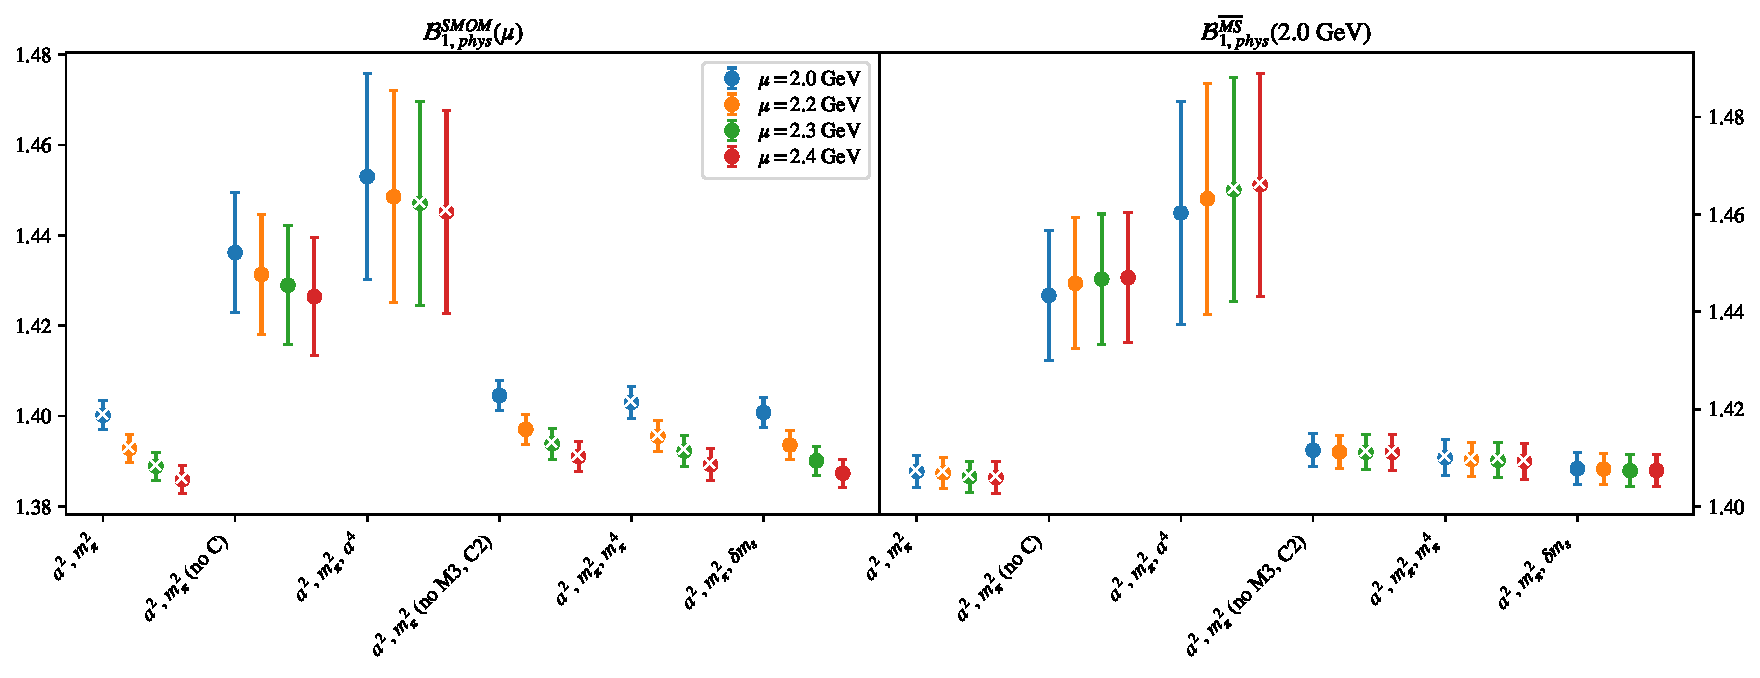
\includegraphics[page=1, width=1.1\textwidth]{VVpAA/NPR/fit_summary_bag.pdf}
\caption{$\mathcal{B}_{1}$\\(left) $\mathcal{B}_{phys}$ in RI/SMOM scheme from fit variations (fits with $p$-value $<0.05$ marked with ``$\times$"). \\(right) $\mathcal{B}_{phys}$ in $\overline{MS}$ computed using $\mathcal{B}^{\overline{MS}} = R^{\overline{MS}\leftarrow SMOM}(2.0)\sigma_{npt}(2.0,\mu) \mathcal{B}^{SMOM}(\mu)$.}
\end{figure}
\clearpage
\begin{figure}
\centering
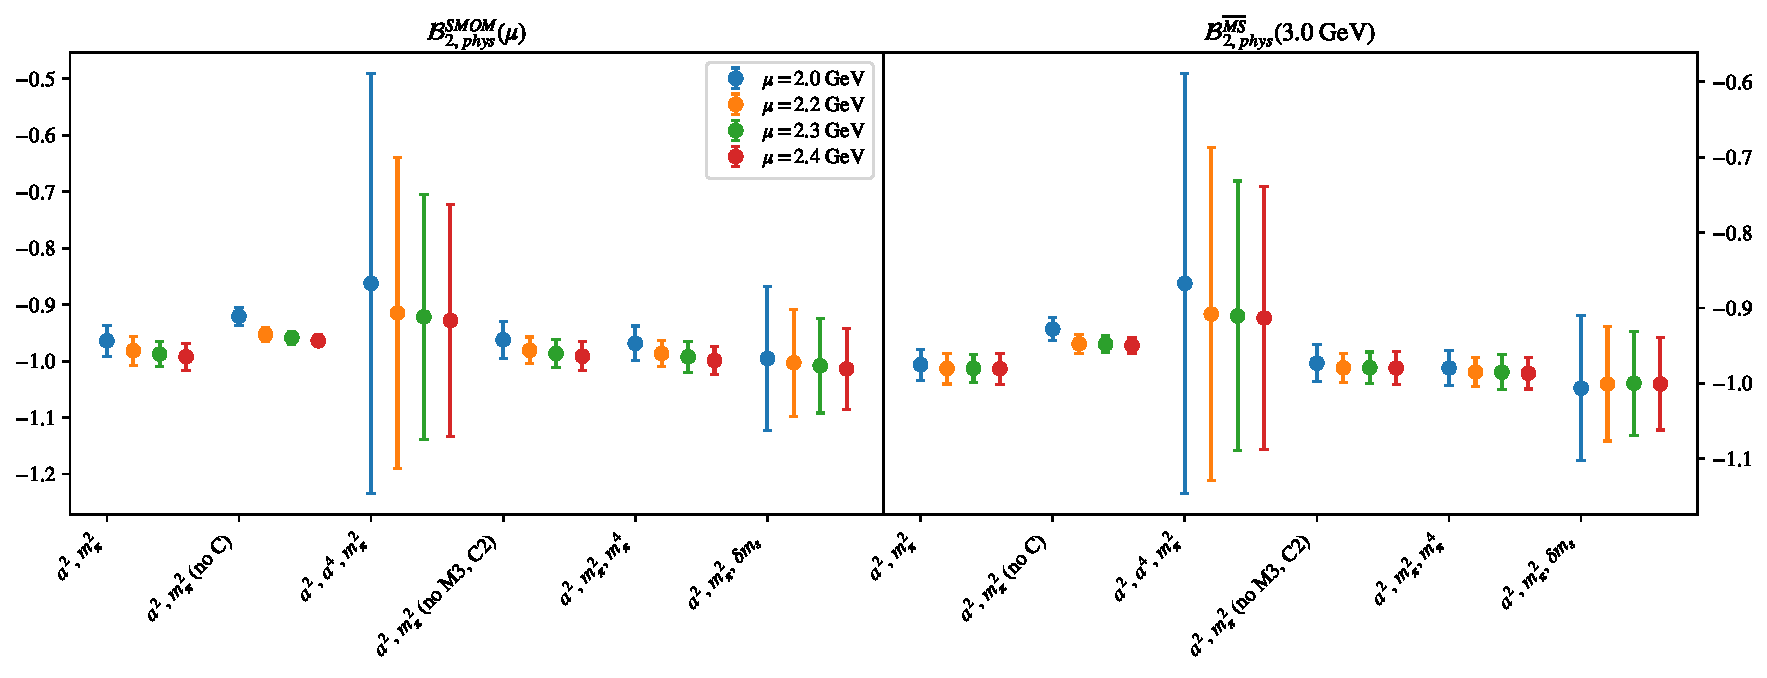
\includegraphics[page=1, width=1.1\textwidth]{VVmAA/NPR/fit_summary_bag.pdf}
\caption{$\mathcal{B}_{2}$\\(left) $\mathcal{B}_{phys}$ in RI/SMOM scheme from fit variations (fits with $p$-value $<0.05$ marked with ``$\times$"). \\(right) $\mathcal{B}_{phys}$ in $\overline{MS}$ computed using $\mathcal{B}^{\overline{MS}} = R^{\overline{MS}\leftarrow SMOM}(3.0)\sigma_{npt}(3.0,\mu) \mathcal{B}^{SMOM}(\mu)$.}
\end{figure}
\clearpage
\begin{figure}
\centering
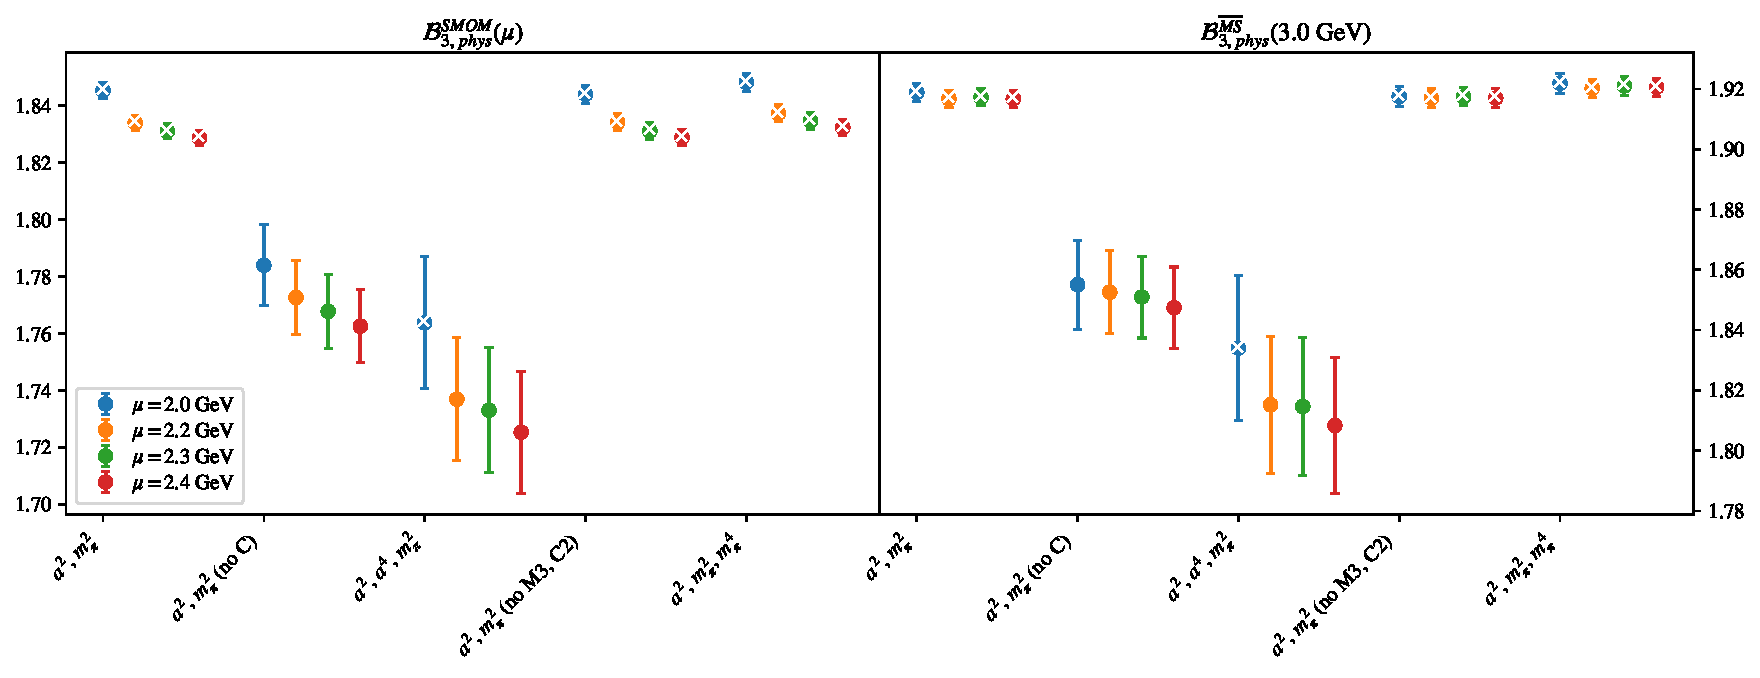
\includegraphics[page=1, width=1.1\textwidth]{SSmPP/NPR/fit_summary_bag.pdf}
\caption{$\mathcal{B}_{3}$\\(left) $\mathcal{B}_{phys}$ in RI/SMOM scheme from fit variations (fits with $p$-value $<0.05$ marked with ``$\times$"). \\(right) $\mathcal{B}_{phys}$ in $\overline{MS}$ computed using $\mathcal{B}^{\overline{MS}} = R^{\overline{MS}\leftarrow SMOM}(3.0)\sigma_{npt}(3.0,\mu) \mathcal{B}^{SMOM}(\mu)$.}
\end{figure}
\clearpage
\begin{figure}
\centering
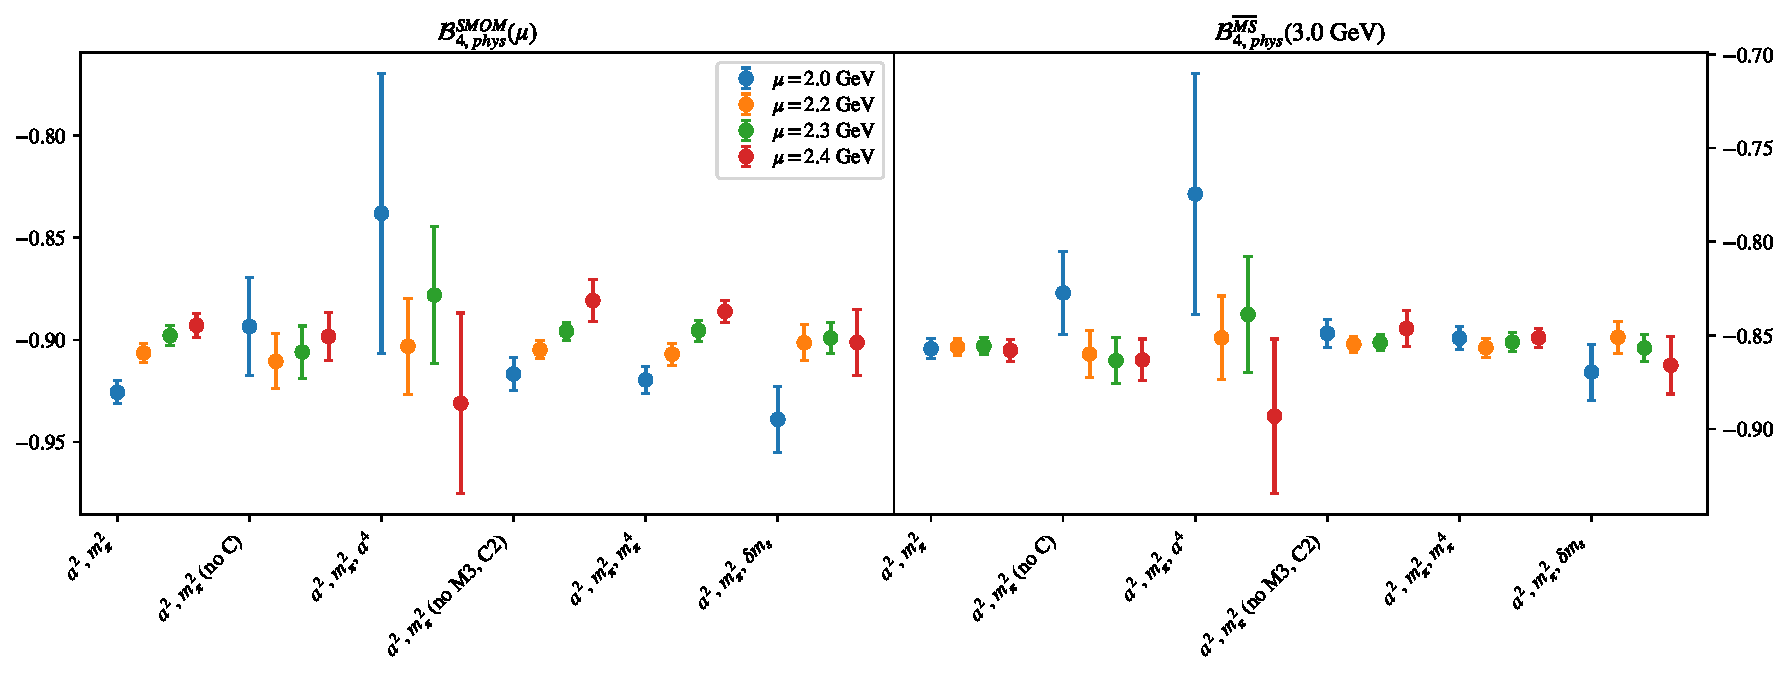
\includegraphics[page=1, width=1.1\textwidth]{SSpPP/NPR/fit_summary_bag.pdf}
\caption{$\mathcal{B}_{4}$\\(left) $\mathcal{B}_{phys}$ in RI/SMOM scheme from fit variations (fits with $p$-value $<0.05$ marked with ``$\times$"). \\(right) $\mathcal{B}_{phys}$ in $\overline{MS}$ computed using $\mathcal{B}^{\overline{MS}} = R^{\overline{MS}\leftarrow SMOM}(3.0)\sigma_{npt}(3.0,\mu) \mathcal{B}^{SMOM}(\mu)$.}
\end{figure}
\clearpage
\begin{figure}
\centering
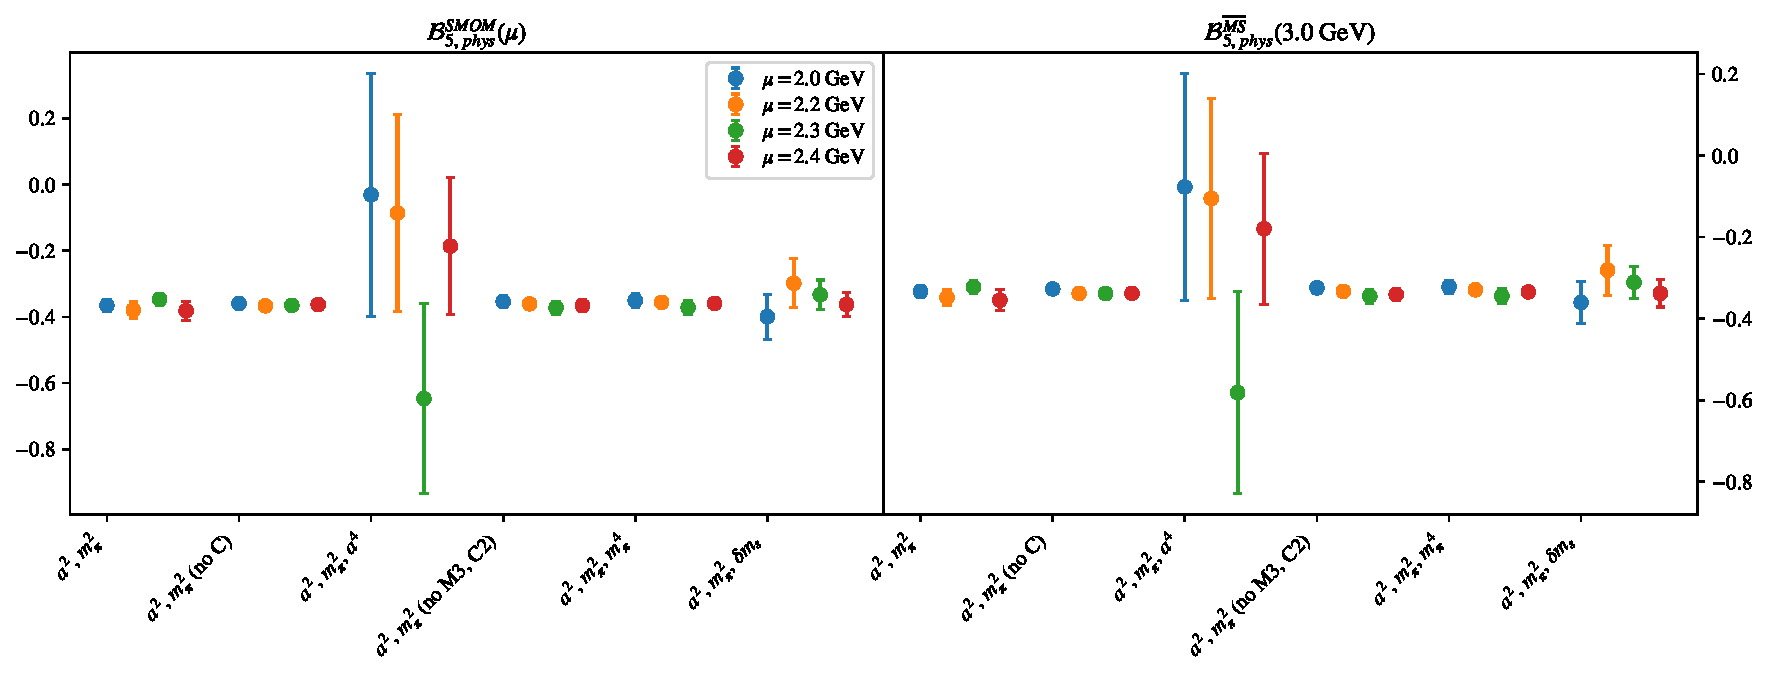
\includegraphics[page=1, width=1.1\textwidth]{TT/NPR/fit_summary_bag.pdf}
\caption{$\mathcal{B}_{5}$\\(left) $\mathcal{B}_{phys}$ in RI/SMOM scheme from fit variations (fits with $p$-value $<0.05$ marked with ``$\times$"). \\(right) $\mathcal{B}_{phys}$ in $\overline{MS}$ computed using $\mathcal{B}^{\overline{MS}} = R^{\overline{MS}\leftarrow SMOM}(3.0)\sigma_{npt}(3.0,\mu) \mathcal{B}^{SMOM}(\mu)$.}
\end{figure}
\clearpage
\section{$\mathcal{B}_1$}
\begin{table}[h!]
\begin{center}
\begin{tabular}{|c|c|c|c|c|c|c|}
\hline
$\mu$ (GeV) & $a^2$, $m_\pi^2$& $a^2$, $m_\pi^2$ (no C)& $a^2$, $a^4$, $m_\pi^2$& $a^2$, $m_\pi^2$ (no M3, C2)& $a^2$, $m_\pi^2$, $m_\pi^4$& $a^2$, $m_\pi^2$, $\delta m_s$\\
\hline
2.0& \hyperlink{VVpAA/NPR/a2m2_20.pdf.1}{\textbf{1.4034(69)}: 0.876 (0.496)} & \hyperlink{VVpAA/NPR/a2m2noC_20.pdf.1}{\textbf{1.413(13)}: 0.977 (0.377)} & \hyperlink{VVpAA/NPR/a2a4m2_20.pdf.1}{\textbf{1.423(24)}: 0.911 (0.456)} & \hyperlink{VVpAA/NPR/a2m2mcut_20.pdf.1}{\textbf{1.4069(65)}: 0.281 (0.839)} & \hyperlink{VVpAA/NPR/a2m2m4_20.pdf.1}{\textbf{1.4074(67)}: 0.605 (0.659)} & \hyperlink{VVpAA/NPR/a2m2delm_20.pdf.1}{\textbf{1.3989(87)}: 0.861 (0.487)}\\
2.2& \hyperlink{VVpAA/NPR/a2m2_22.pdf.1}{\textbf{1.3953(57)}: 1.207 (0.303)} & \hyperlink{VVpAA/NPR/a2m2noC_22.pdf.1}{\textbf{1.410(13)}: 1.024 (0.359)} & \hyperlink{VVpAA/NPR/a2a4m2_22.pdf.1}{\textbf{1.424(23)}: 1.113 (0.348)} & \hyperlink{VVpAA/NPR/a2m2mcut_22.pdf.1}{\textbf{1.3998(59)}: 0.519 (0.669)} & \hyperlink{VVpAA/NPR/a2m2m4_22.pdf.1}{\textbf{1.3996(65)}: 0.94 (0.439)} & \hyperlink{VVpAA/NPR/a2m2delm_22.pdf.1}{\textbf{1.3908(78)}: 0.915 (0.454)}\\
2.3& \hyperlink{VVpAA/NPR/a2m2_23.pdf.1}{\textbf{1.3922(60)}: 1.298 (0.262)} & \hyperlink{VVpAA/NPR/a2m2noC_23.pdf.1}{\textbf{1.409(13)}: 1.046 (0.351)} & \hyperlink{VVpAA/NPR/a2a4m2_23.pdf.1}{\textbf{1.425(24)}: 1.019 (0.396)} & \hyperlink{VVpAA/NPR/a2m2mcut_23.pdf.1}{\textbf{1.3970(62)}: 0.627 (0.597)} & \hyperlink{VVpAA/NPR/a2m2m4_23.pdf.1}{\textbf{1.3961(64)}: 1.151 (0.33)} & \hyperlink{VVpAA/NPR/a2m2delm_23.pdf.1}{\textbf{1.3871(74)}: 1.015 (0.398)}\\
2.4& \hyperlink{VVpAA/NPR/a2m2_24.pdf.1}{\textbf{1.3893(59)}: 1.348 (0.241)} & \hyperlink{VVpAA/NPR/a2m2noC_24.pdf.1}{\textbf{1.407(13)}: 1.072 (0.342)} & \hyperlink{VVpAA/NPR/a2a4m2_24.pdf.1}{\textbf{1.424(24)}: 1.101 (0.354)} & \hyperlink{VVpAA/NPR/a2m2mcut_24.pdf.1}{\textbf{1.3939(58)}: 0.692 (0.557)} & \hyperlink{VVpAA/NPR/a2m2m4_24.pdf.1}{\textbf{1.3930(64)}: 1.184 (0.316)} & \hyperlink{VVpAA/NPR/a2m2delm_24.pdf.1}{\textbf{1.3832(77)}: 0.911 (0.456)}\\
\hline
\end{tabular}
\caption{Physical point value from chiral and continuum extrapolation at renormalisation scale $\mu$. Entries are \textbf{value(error)}: $\chi^2/\text{DOF}$ ($p$-value).}
\end{center}
\end{table}
\begin{table}[h!]
\begin{center}
\begin{tabular}{|c c|c|c|c|c|c|c|}
\hline
$\mu$ (GeV) &  & $a^2$, $m_\pi^2$& $a^2$, $m_\pi^2$ (no C)& $a^2$, $a^4$, $m_\pi^2$& $a^2$, $m_\pi^2$ (no M3, C2)& $a^2$, $m_\pi^2$, $m_\pi^4$& $a^2$, $m_\pi^2$, $\delta m_s$\\
\hline
\multirow{2}{0.5in}{2.0} & $\alpha$ & 0.103(28)& 0.060(59)& -0.035& 0.093(25)& 0.093(26)& 0.116(33)\\
 & $\beta$ & 0.00233(23)& 0.00226(27)& 0.00234(22)& 0.00186(32)& 0.001& 0.00245(23)\\
\hline
\multirow{2}{0.5in}{2.2} & $\alpha$ & 0.108(23)& 0.044(57)& -0.089& 0.094(22)& 0.096(24)& 0.120(28)\\
 & $\beta$ & 0.00235(21)& 0.00224(27)& 0.00238(20)& 0.00182(31)& 0.001& 0.00249(23)\\
\hline
\multirow{2}{0.5in}{2.3} & $\alpha$ & 0.108(23)& 0.035(56)& -0.1(15)& 0.094(24)& 0.098(24)& 0.121(27)\\
 & $\beta$ & 0.00232(21)& 0.00224(27)& 0.00236(21)& 0.00181(32)& 0.00053(98)& 0.00250(22)\\
\hline
\multirow{2}{0.5in}{2.4} & $\alpha$ & 0.109(23)& 0.032(55)& -0.1(16)& 0.095(22)& 0.099(23)& 0.125(27)\\
 & $\beta$ & 0.00234(21)& 0.00223(27)& 0.00239(20)& 0.00181(31)& 0.00065(96)& 0.00254(21)\\
\hline
\end{tabular}
\caption{Fit values of coefficients in $Q = Q_{phys} + \mathbf{\alpha} a^2 + \mathbf{\beta}\left(\frac{m_\pi^2}{f_\pi^2}-\frac{m_{\pi,PDG}^2}{f_\pi^2}\right) + \ldots$.}
\end{center}
\end{table}
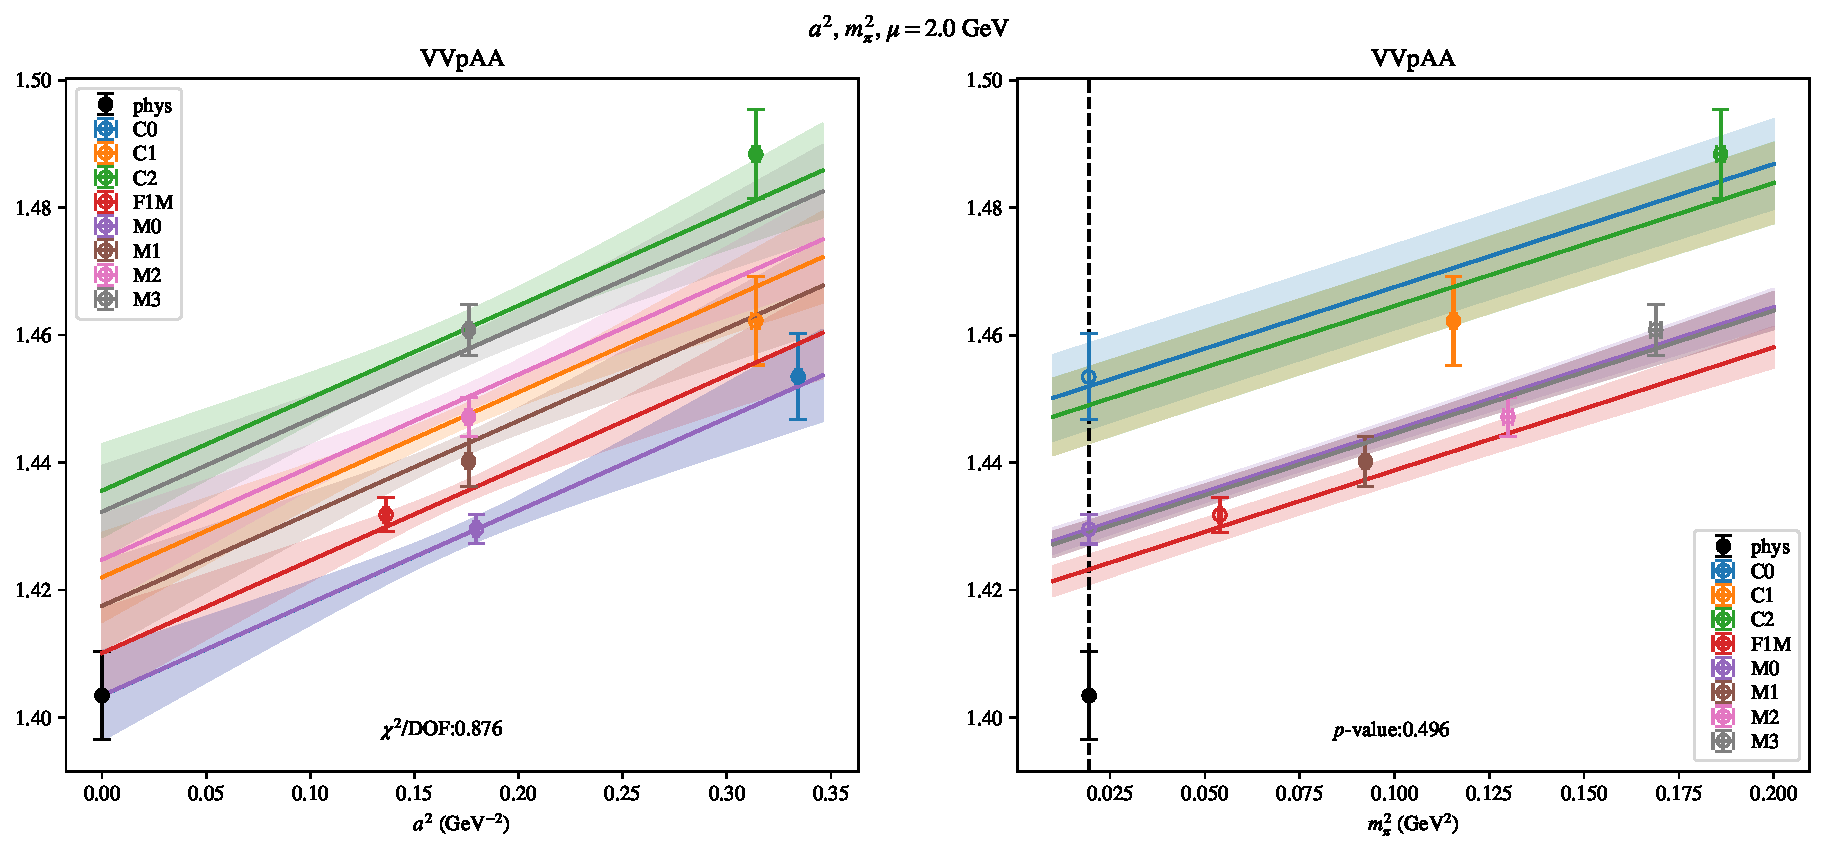
\includepdf[link, pages=-]{VVpAA/NPR/a2m2_20.pdf}
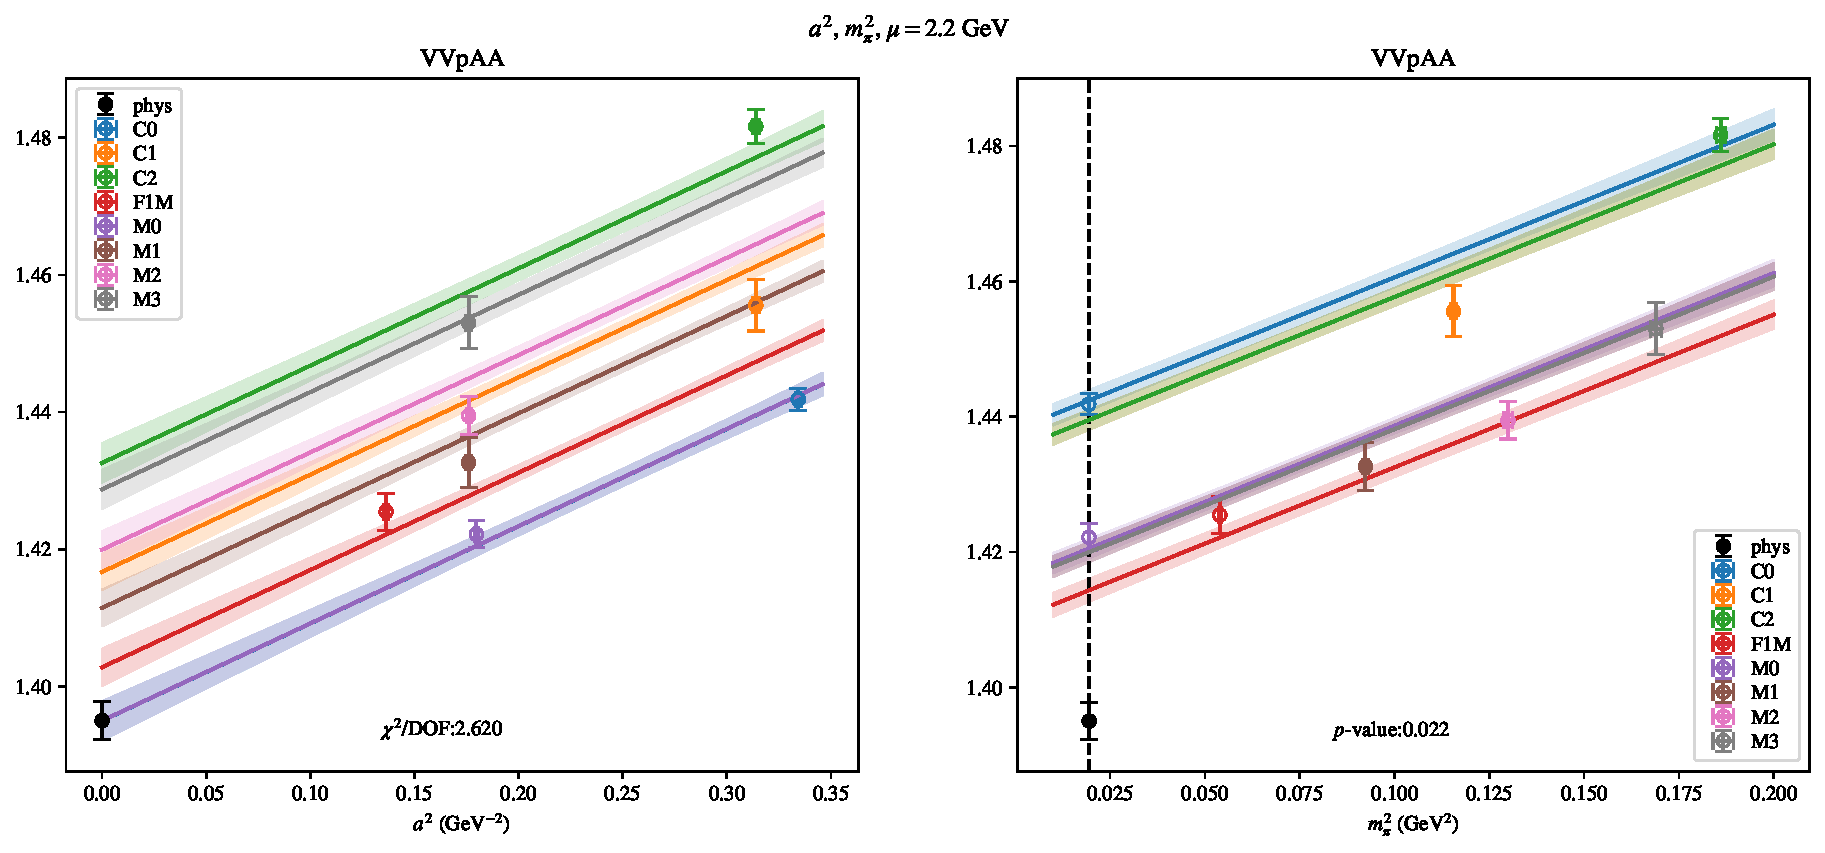
\includepdf[link, pages=-]{VVpAA/NPR/a2m2_22.pdf}
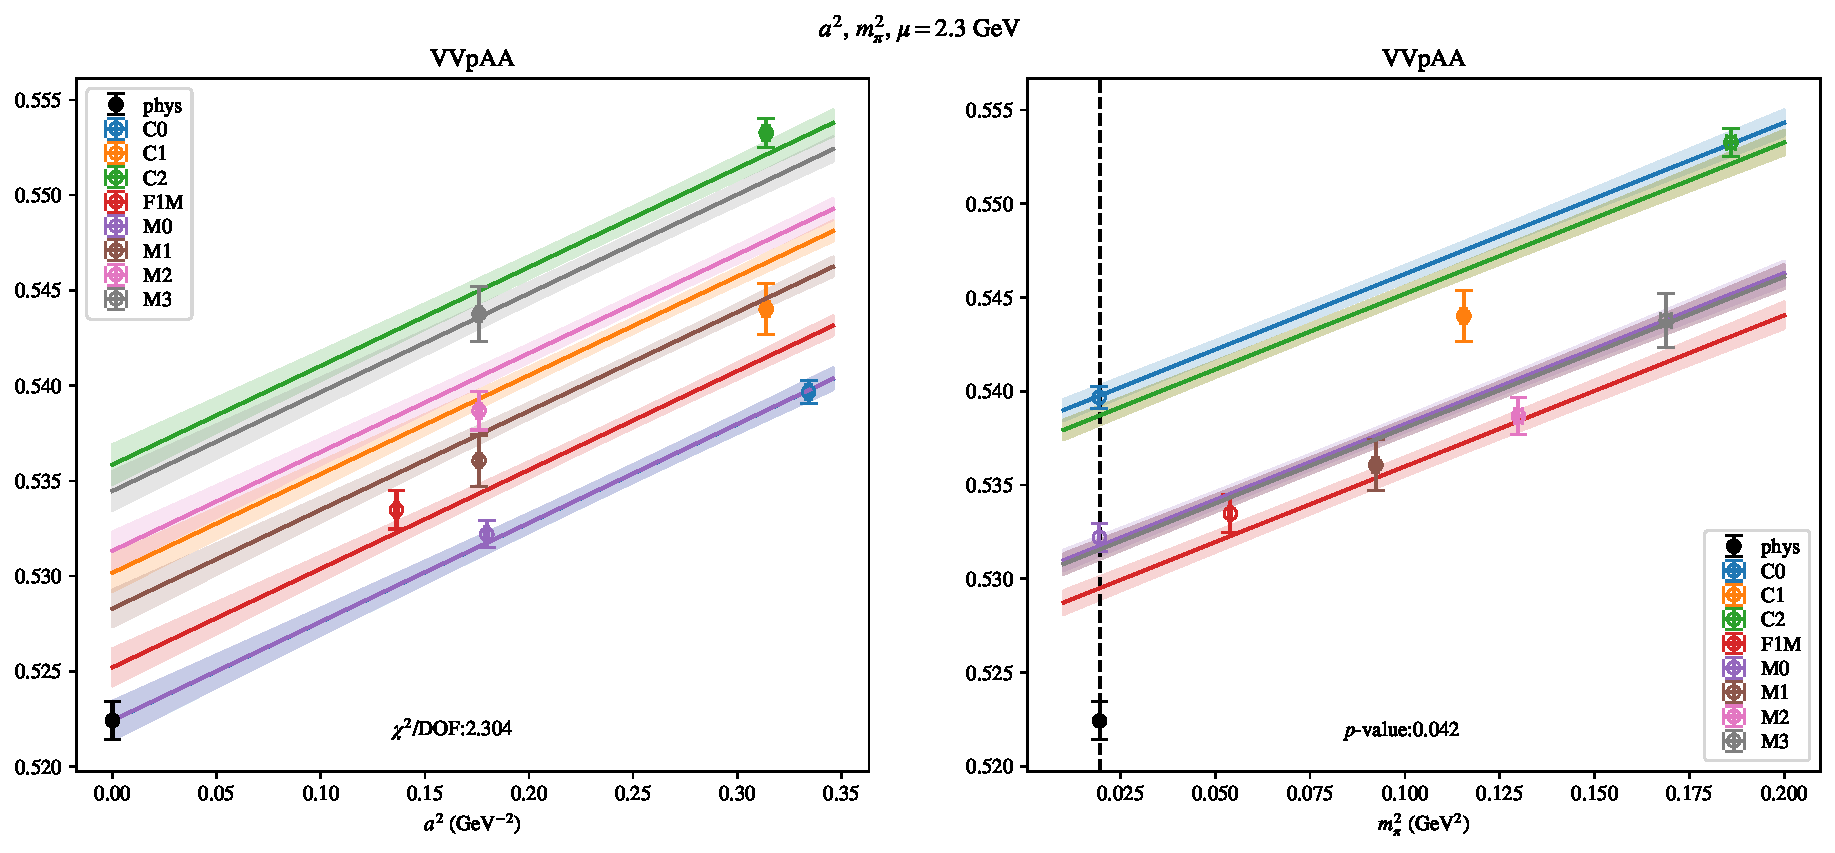
\includepdf[link, pages=-]{VVpAA/NPR/a2m2_23.pdf}
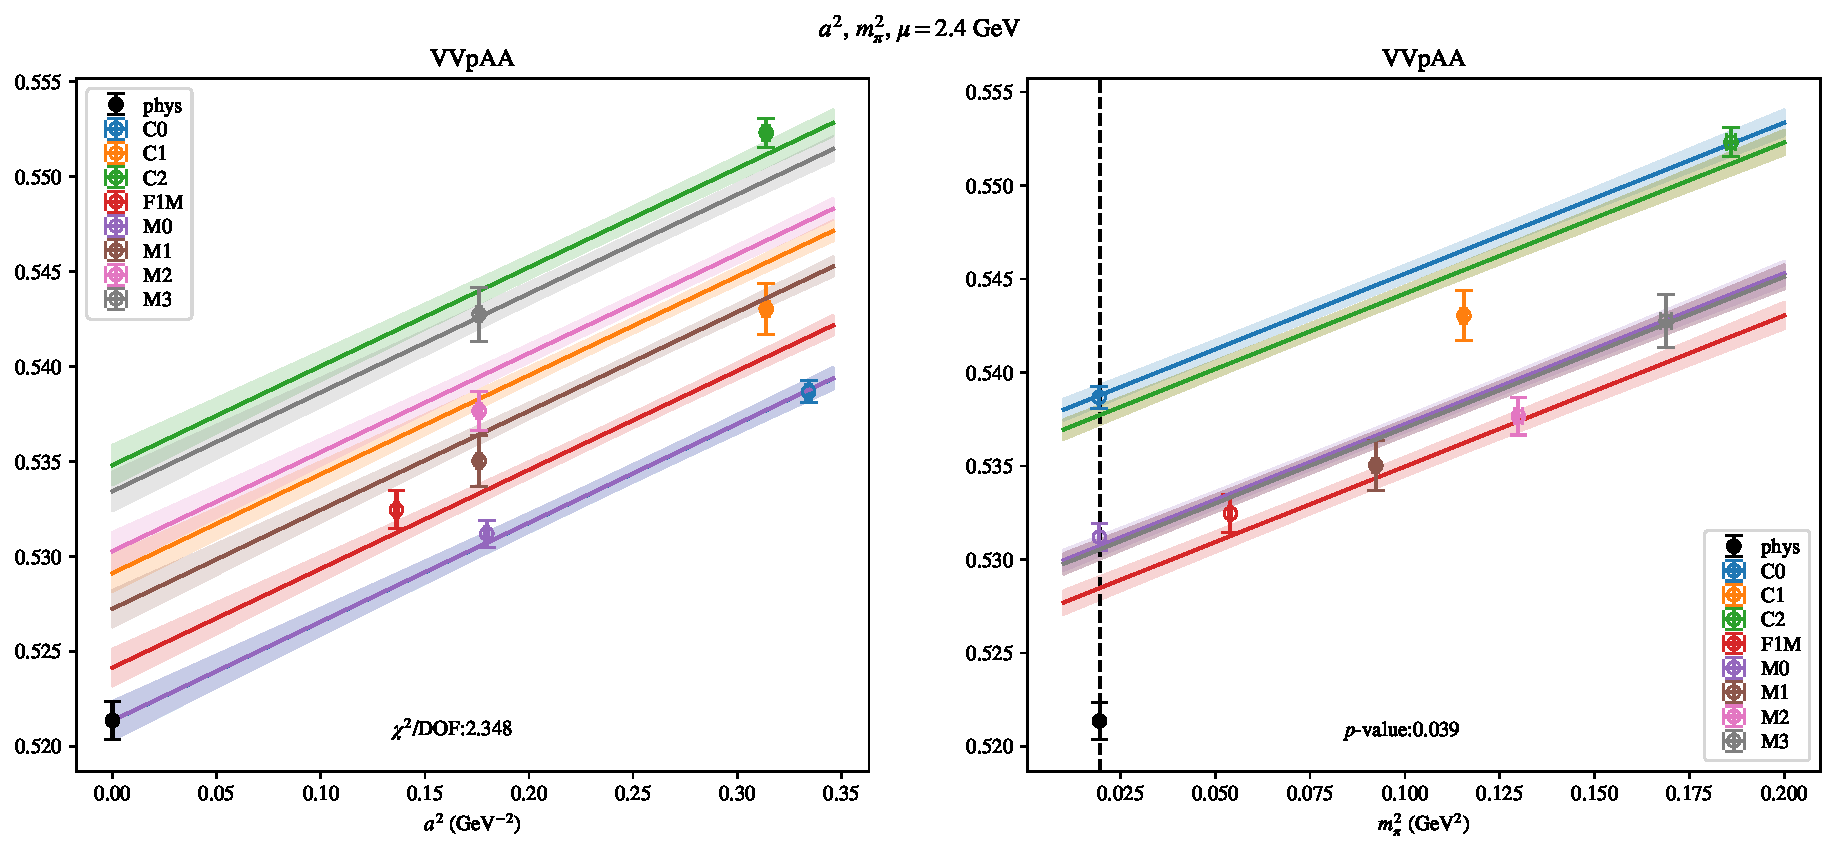
\includepdf[link, pages=-]{VVpAA/NPR/a2m2_24.pdf}
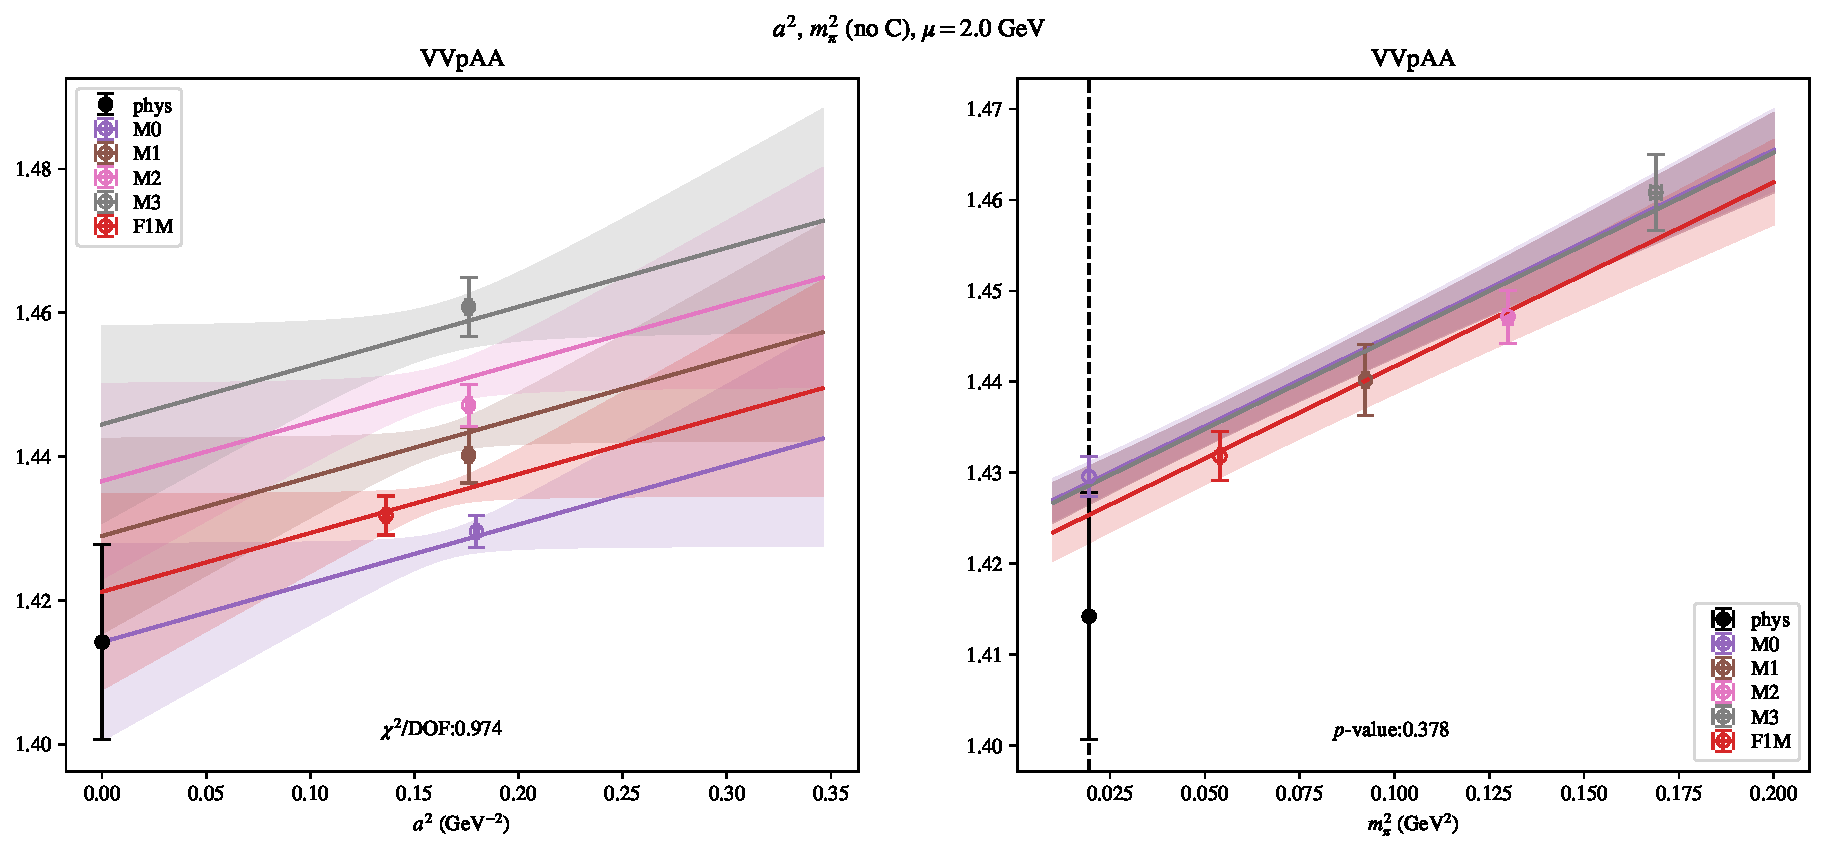
\includepdf[link, pages=-]{VVpAA/NPR/a2m2noC_20.pdf}
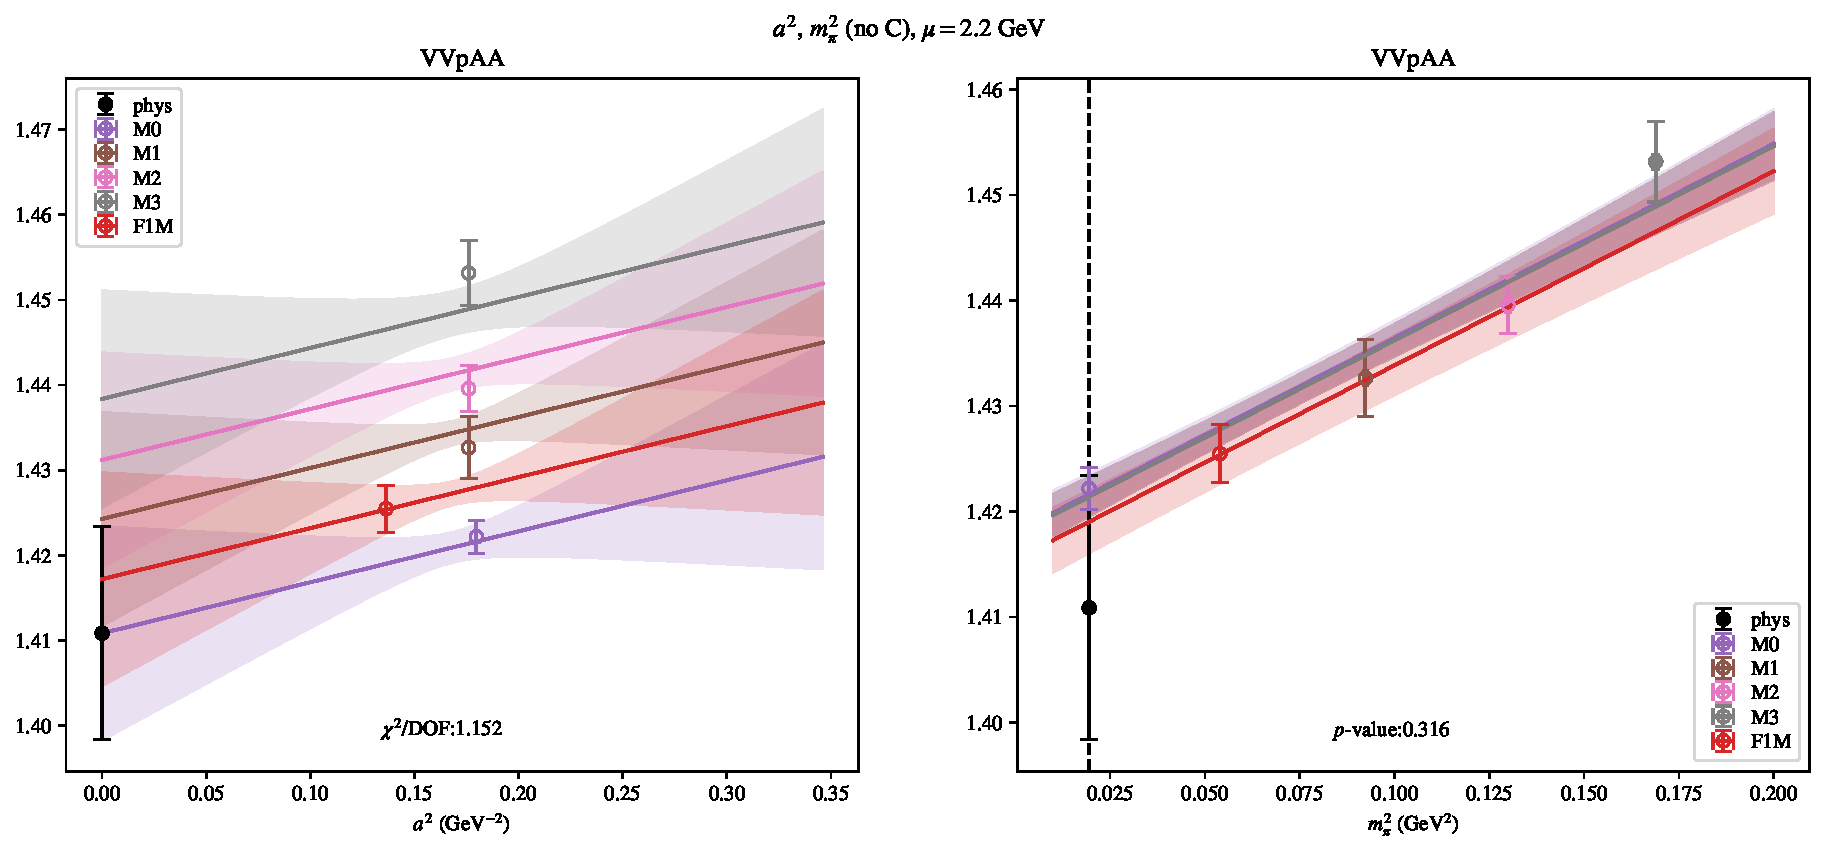
\includepdf[link, pages=-]{VVpAA/NPR/a2m2noC_22.pdf}
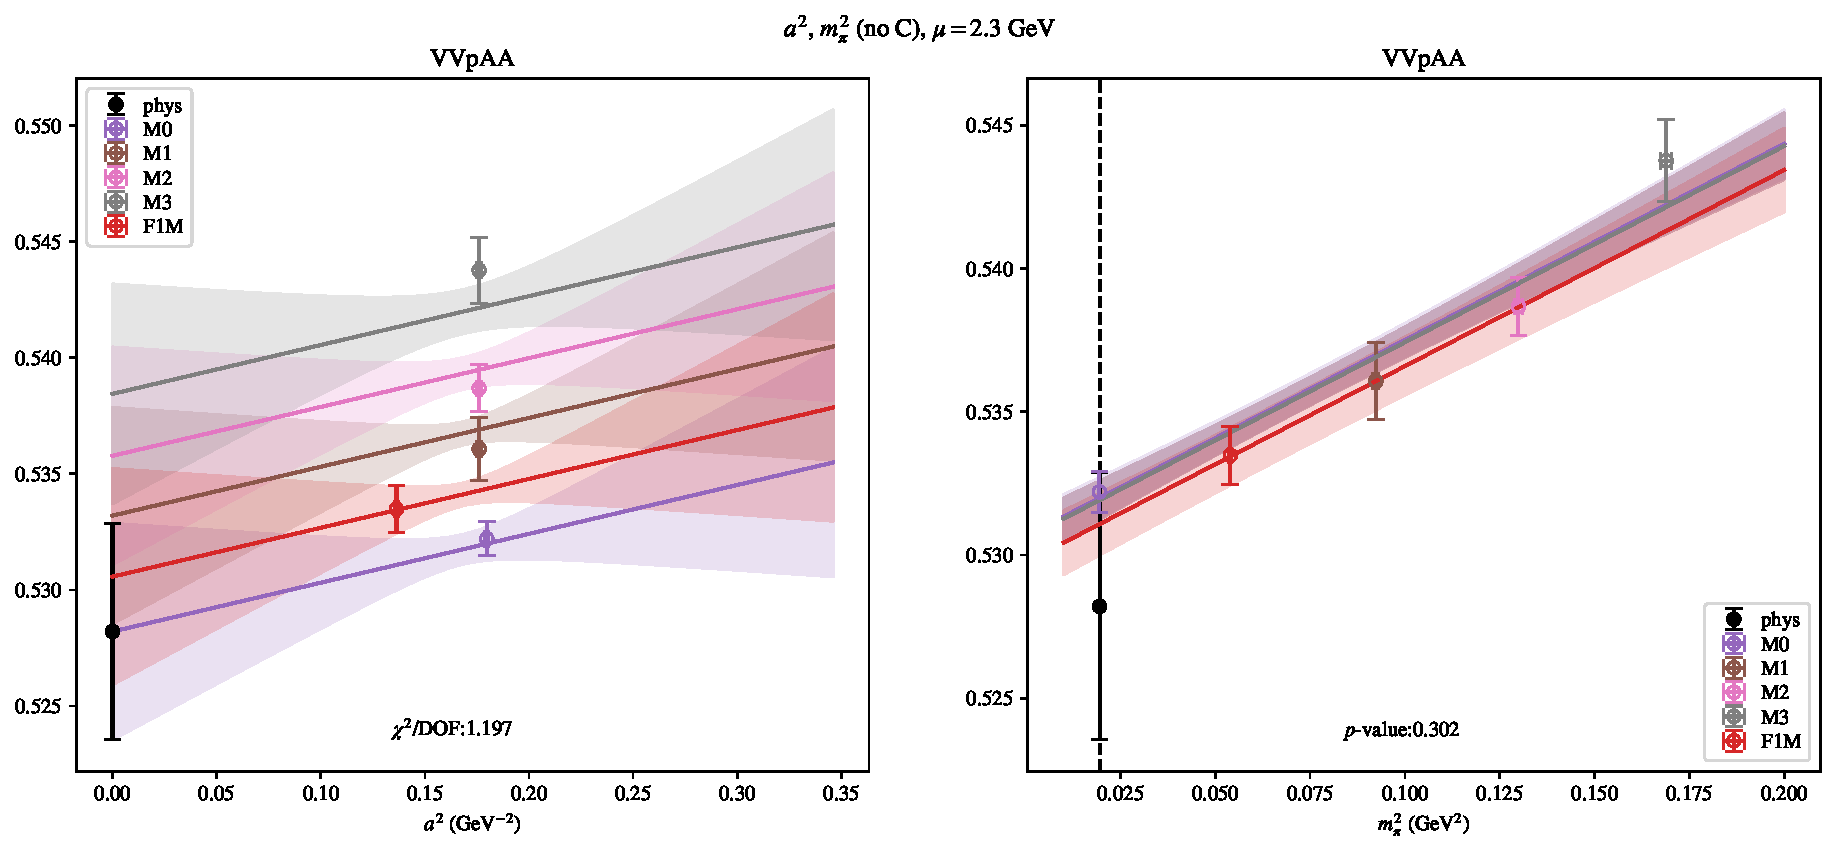
\includepdf[link, pages=-]{VVpAA/NPR/a2m2noC_23.pdf}
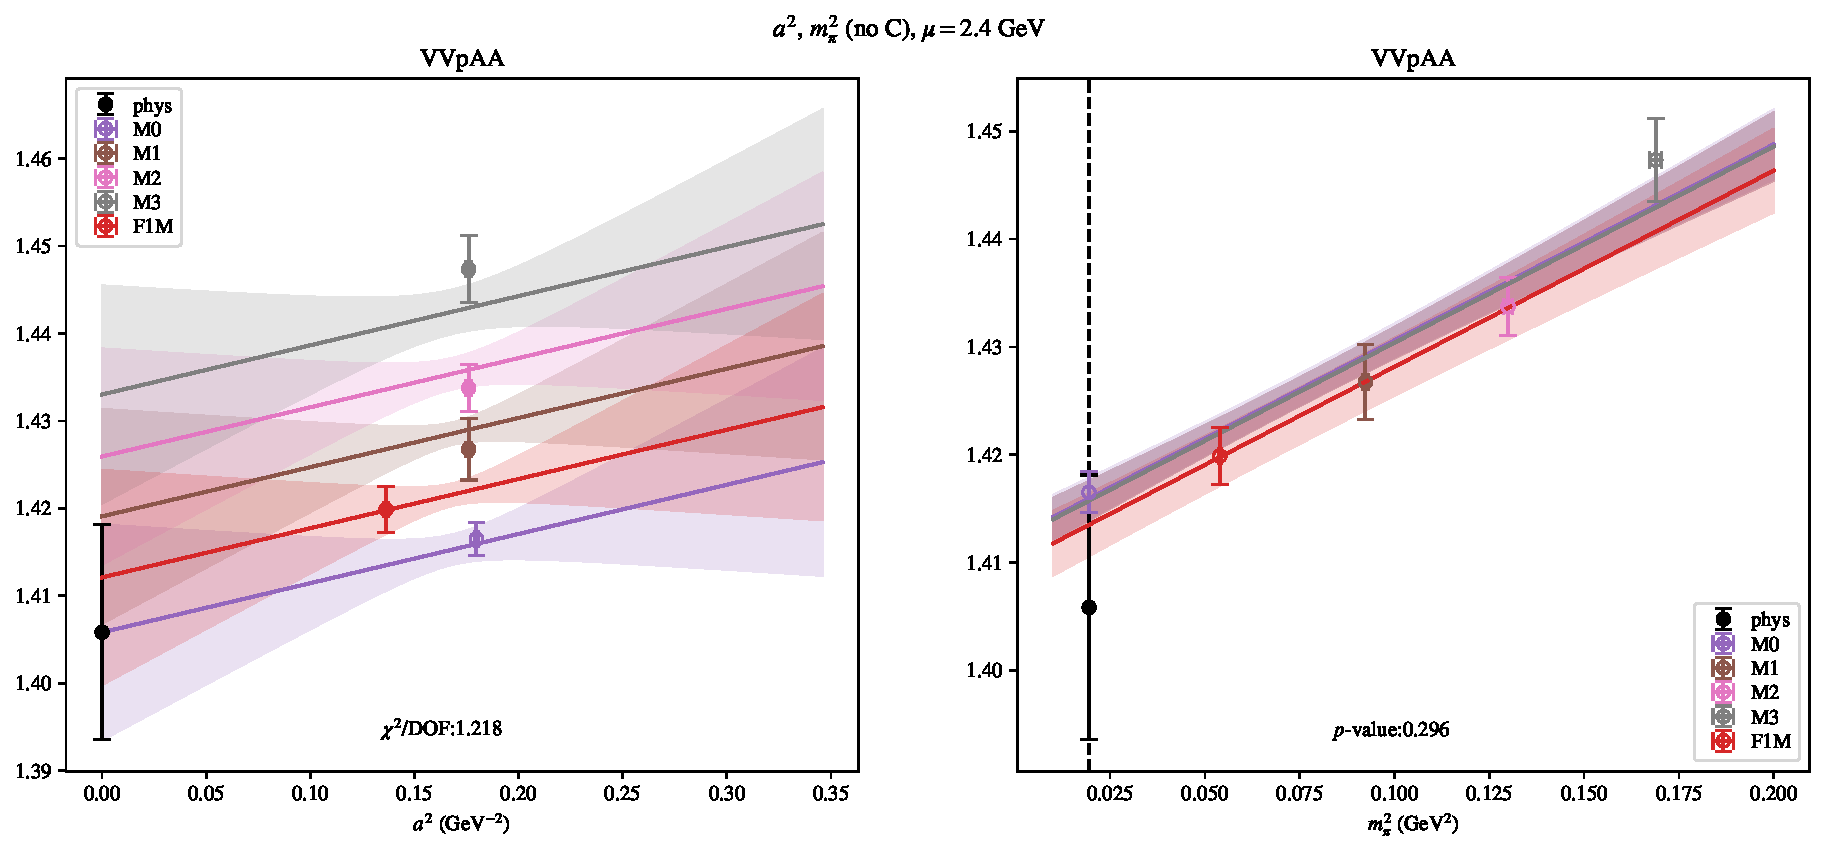
\includepdf[link, pages=-]{VVpAA/NPR/a2m2noC_24.pdf}
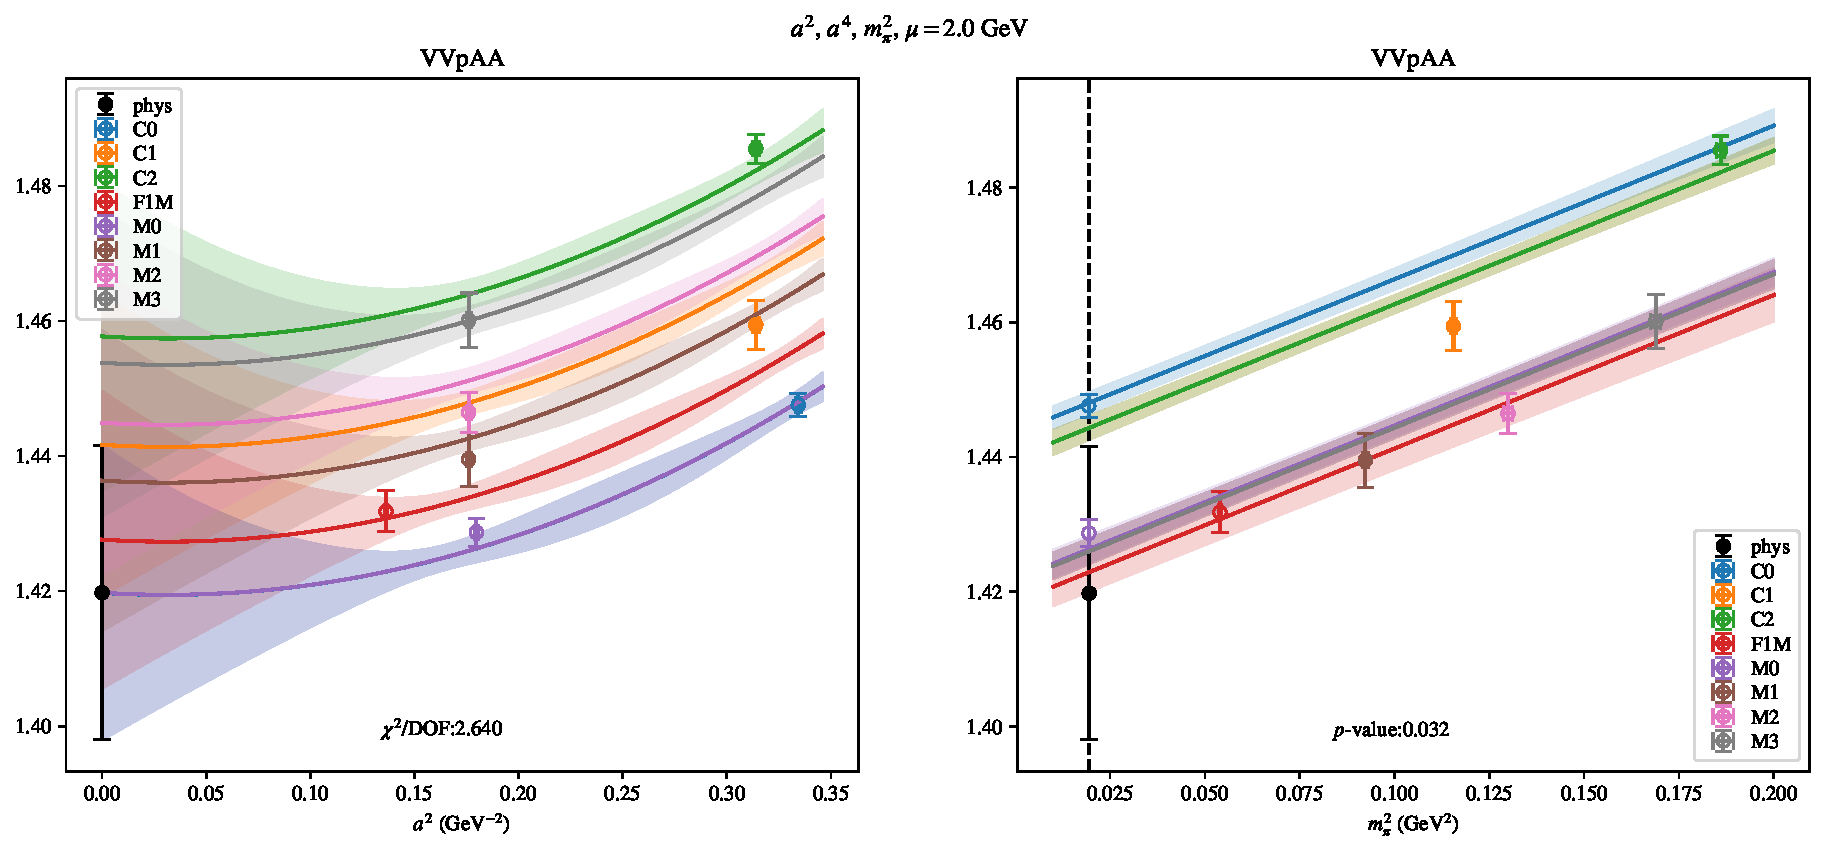
\includepdf[link, pages=-]{VVpAA/NPR/a2a4m2_20.pdf}
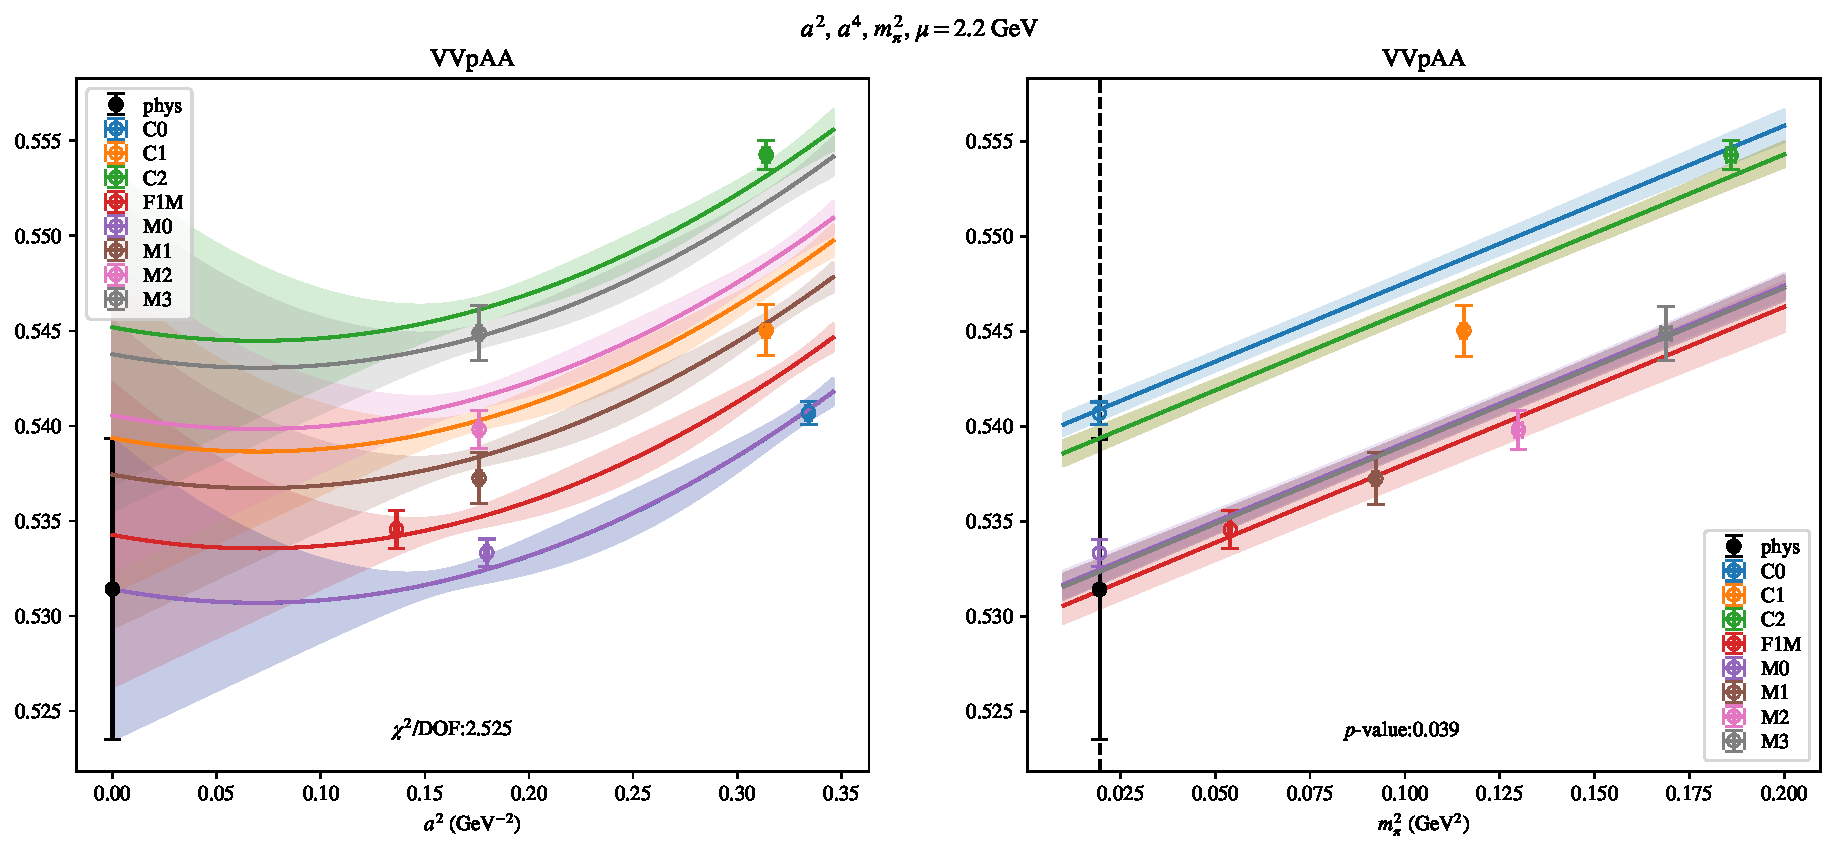
\includepdf[link, pages=-]{VVpAA/NPR/a2a4m2_22.pdf}
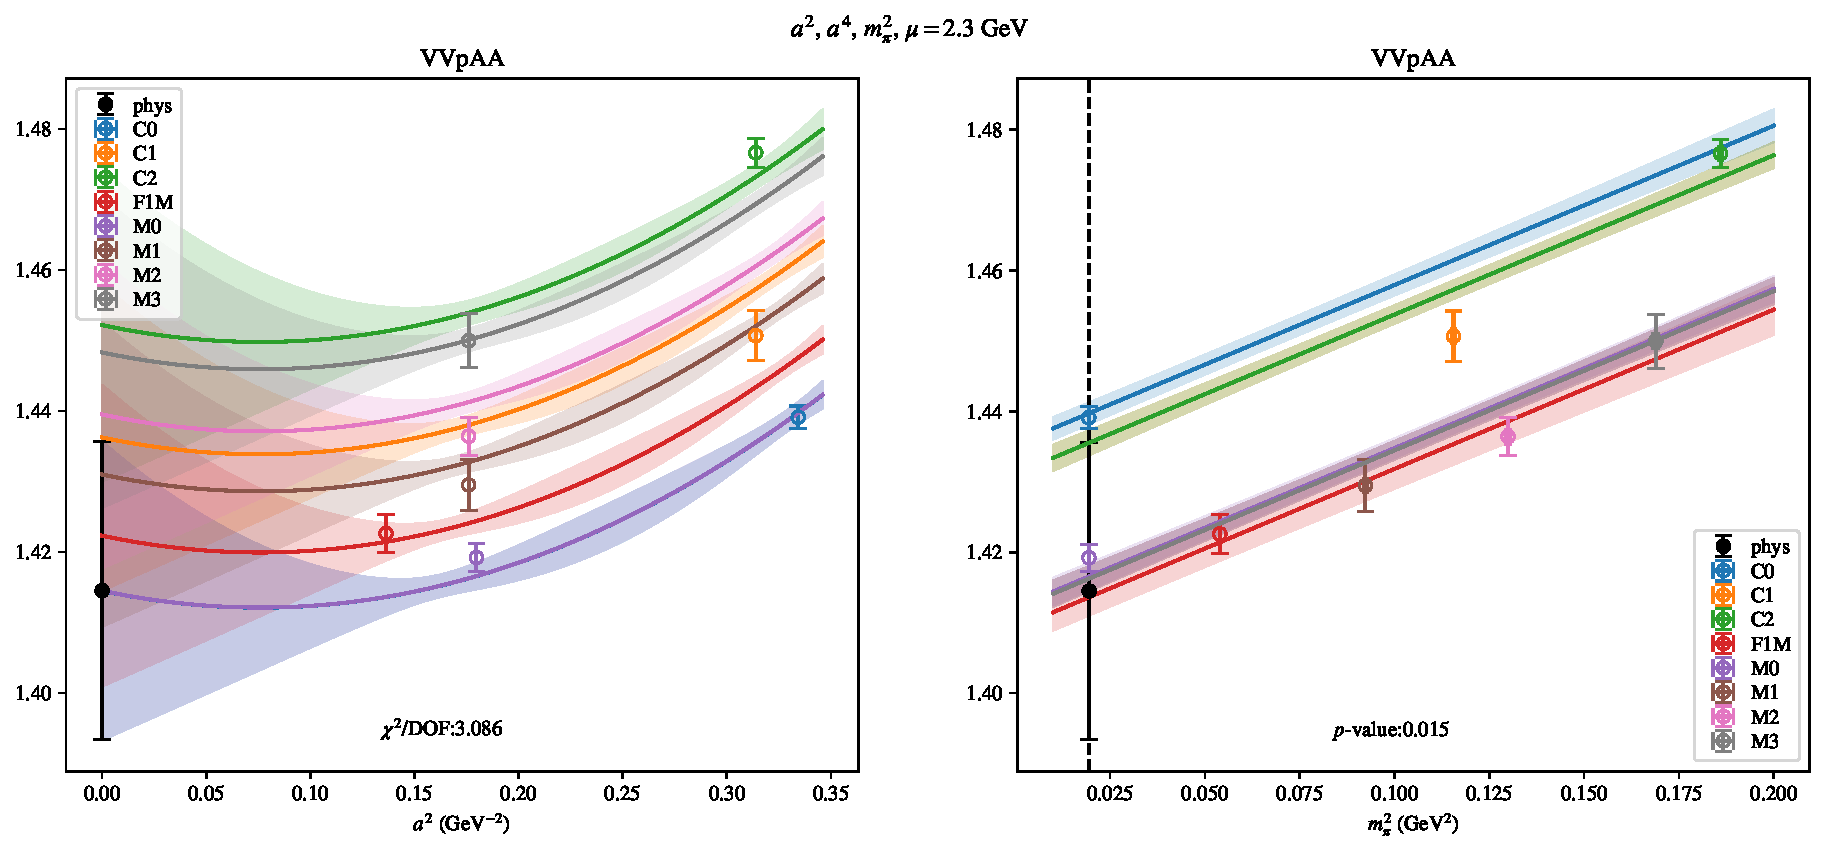
\includepdf[link, pages=-]{VVpAA/NPR/a2a4m2_23.pdf}
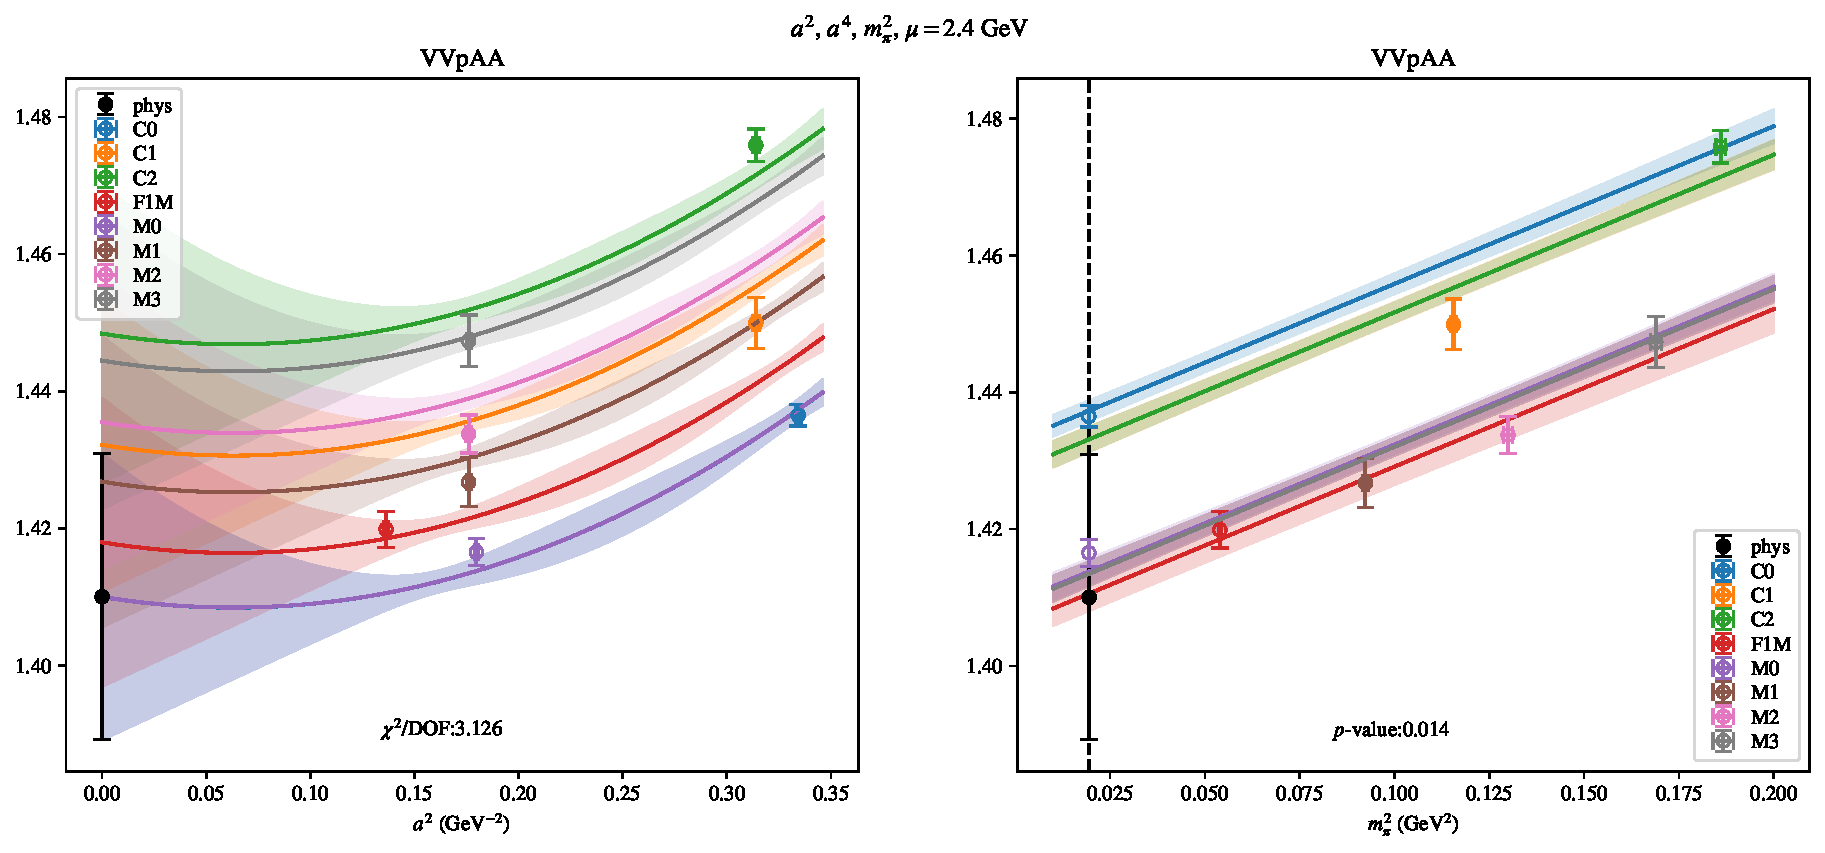
\includepdf[link, pages=-]{VVpAA/NPR/a2a4m2_24.pdf}
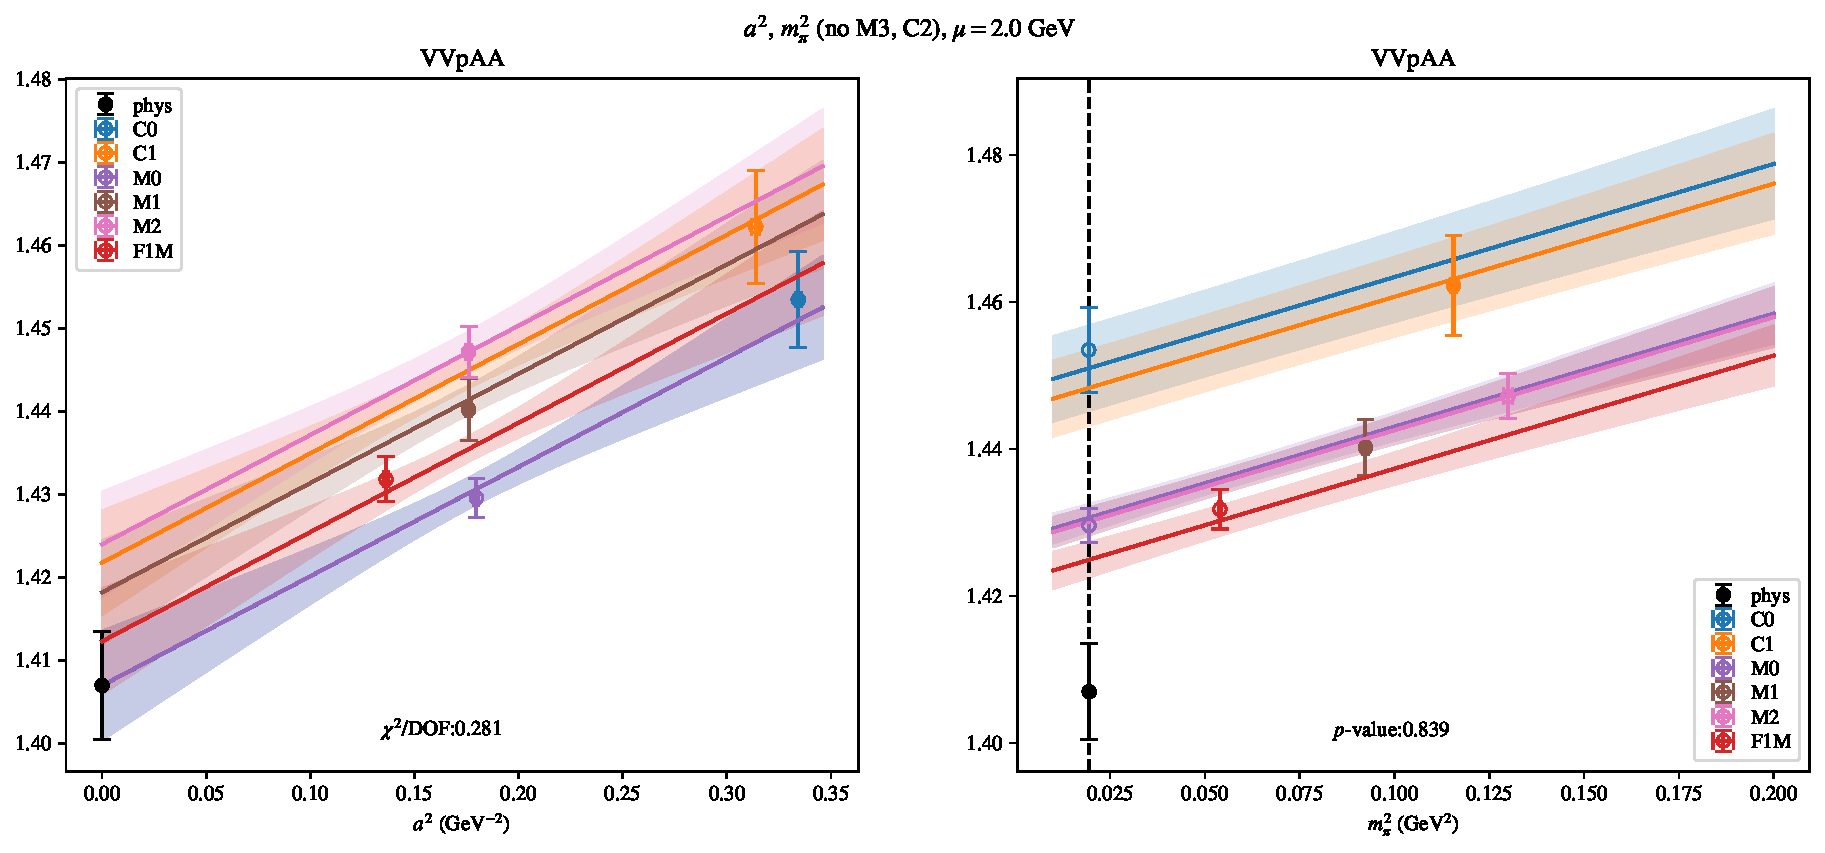
\includepdf[link, pages=-]{VVpAA/NPR/a2m2mcut_20.pdf}
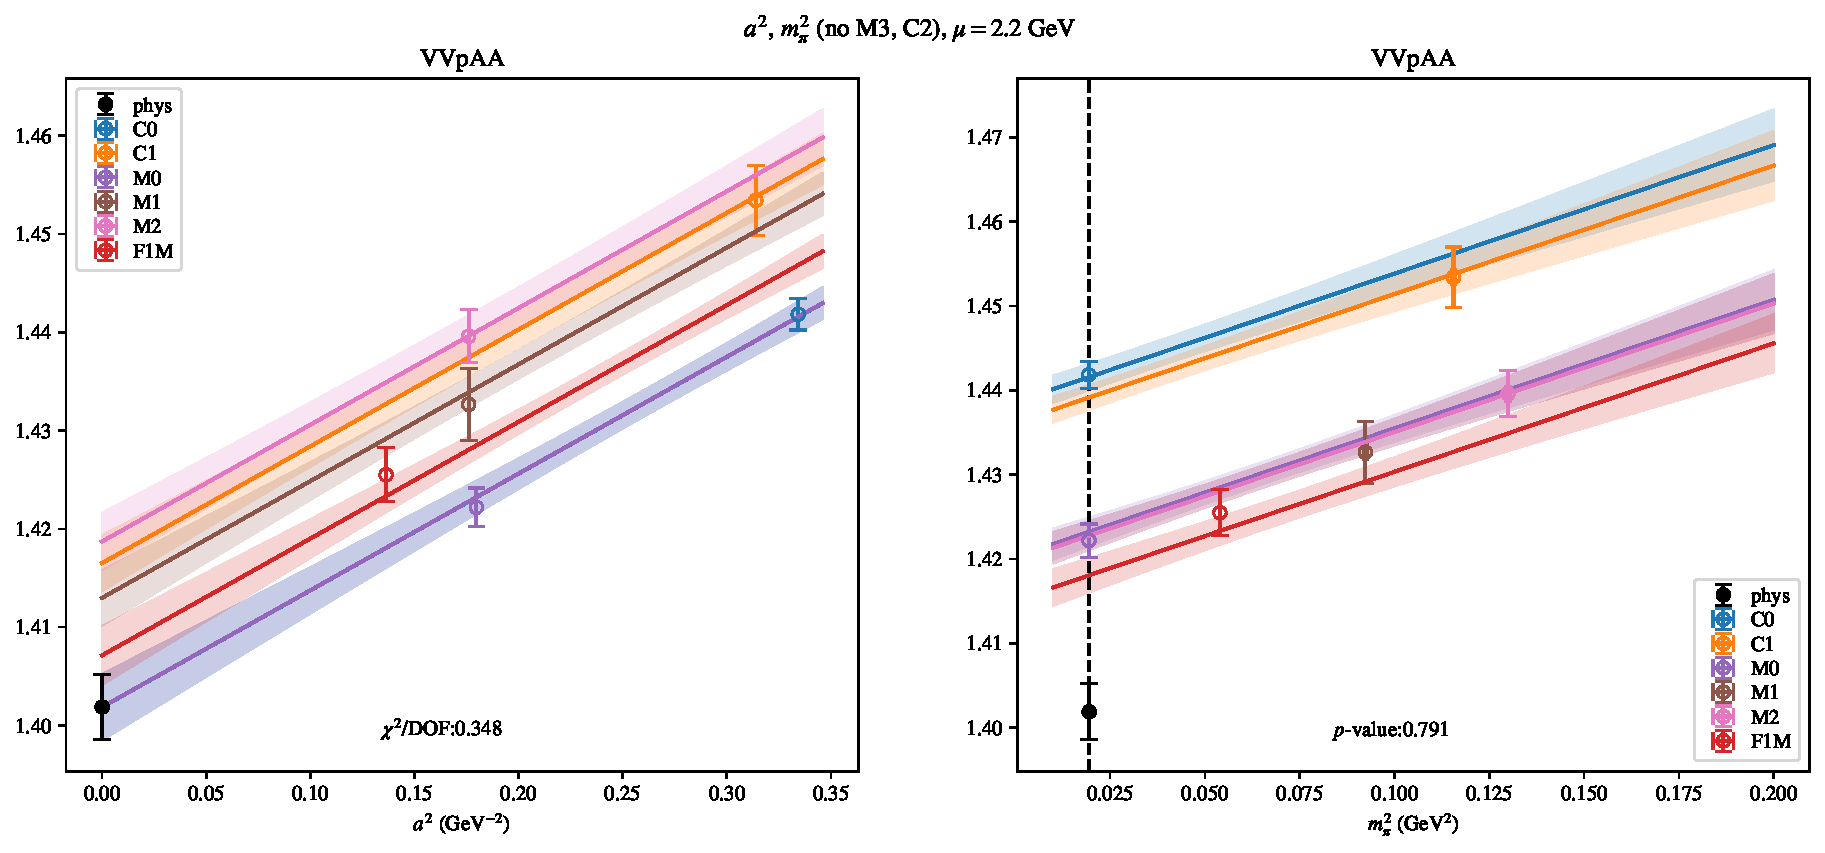
\includepdf[link, pages=-]{VVpAA/NPR/a2m2mcut_22.pdf}
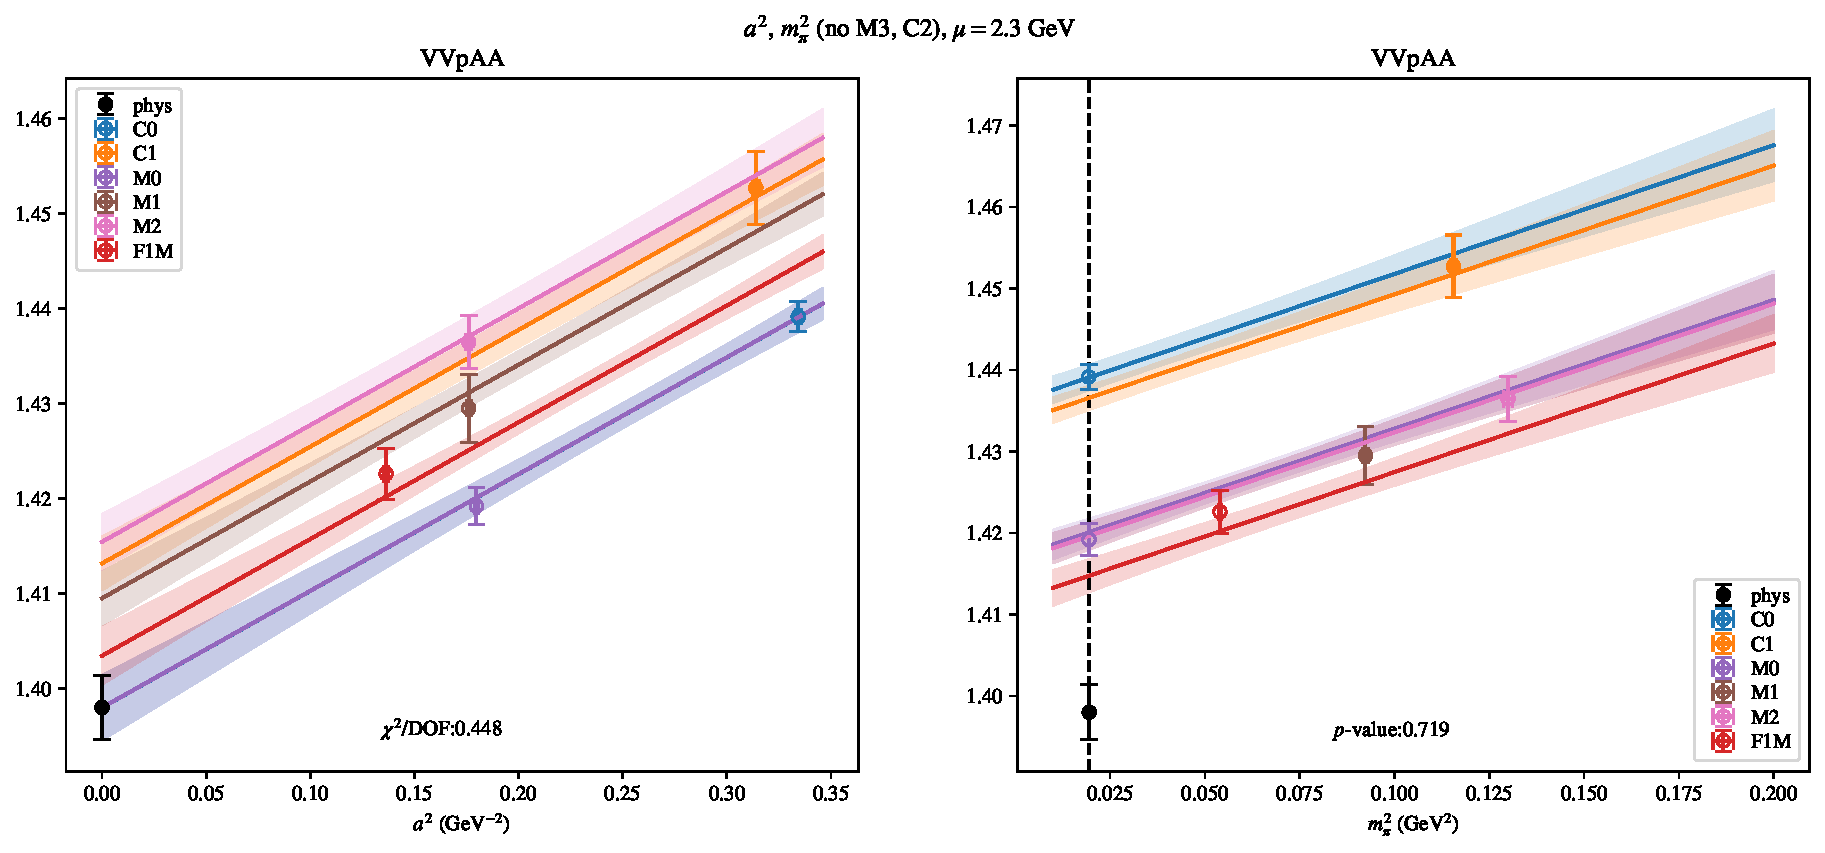
\includepdf[link, pages=-]{VVpAA/NPR/a2m2mcut_23.pdf}
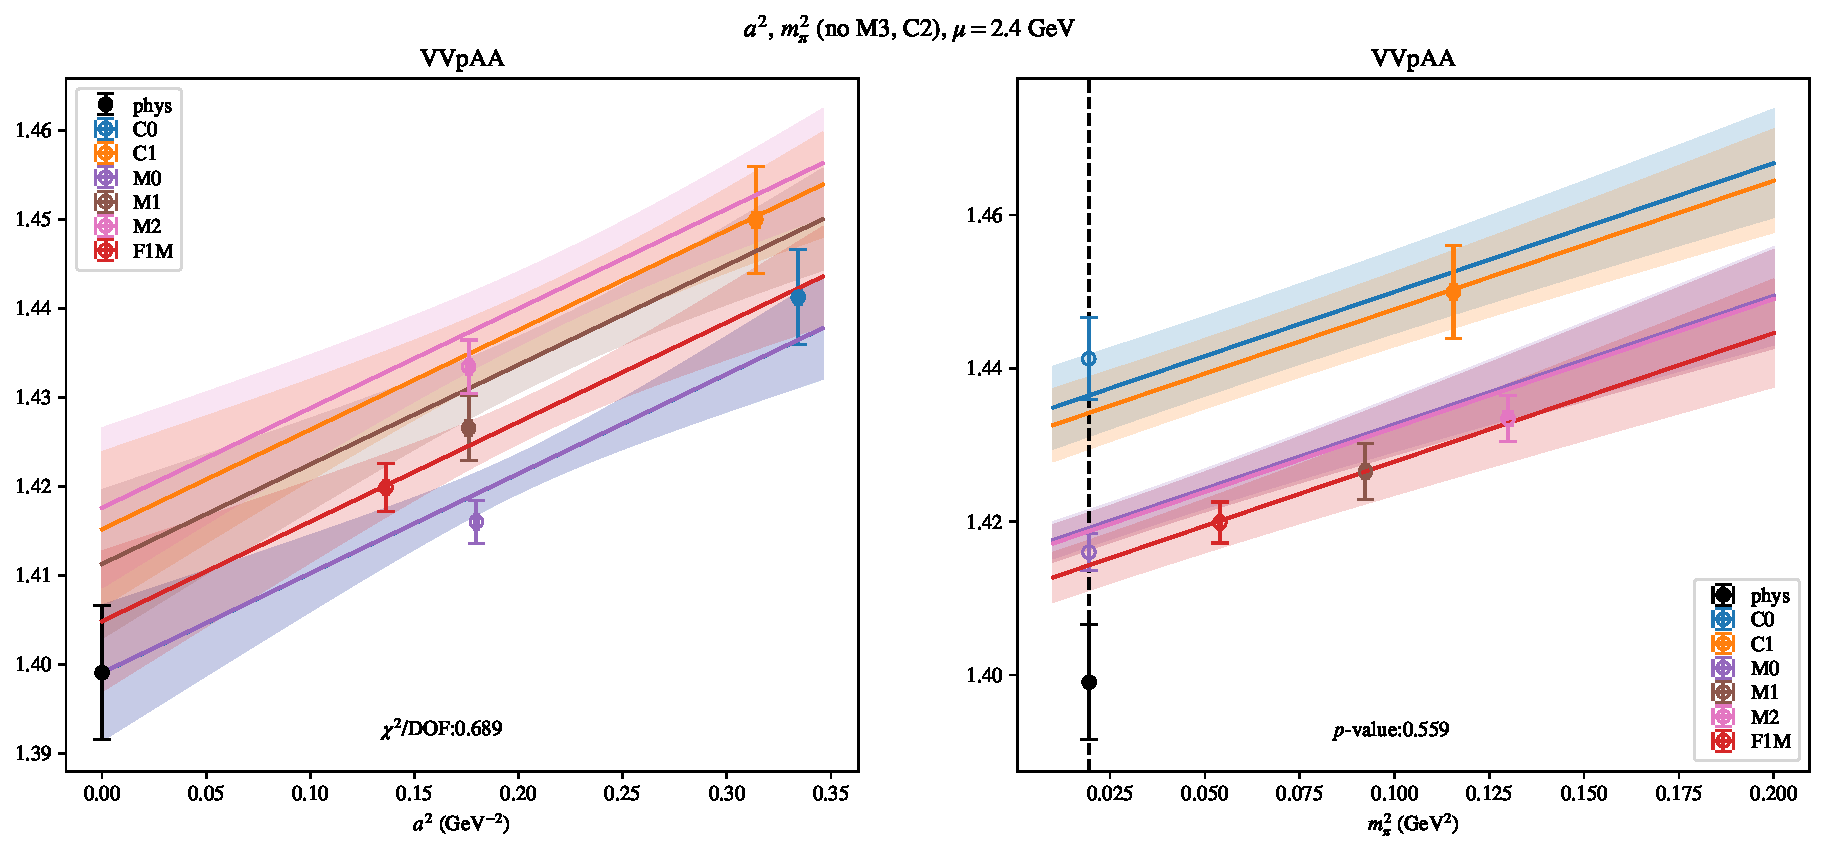
\includepdf[link, pages=-]{VVpAA/NPR/a2m2mcut_24.pdf}
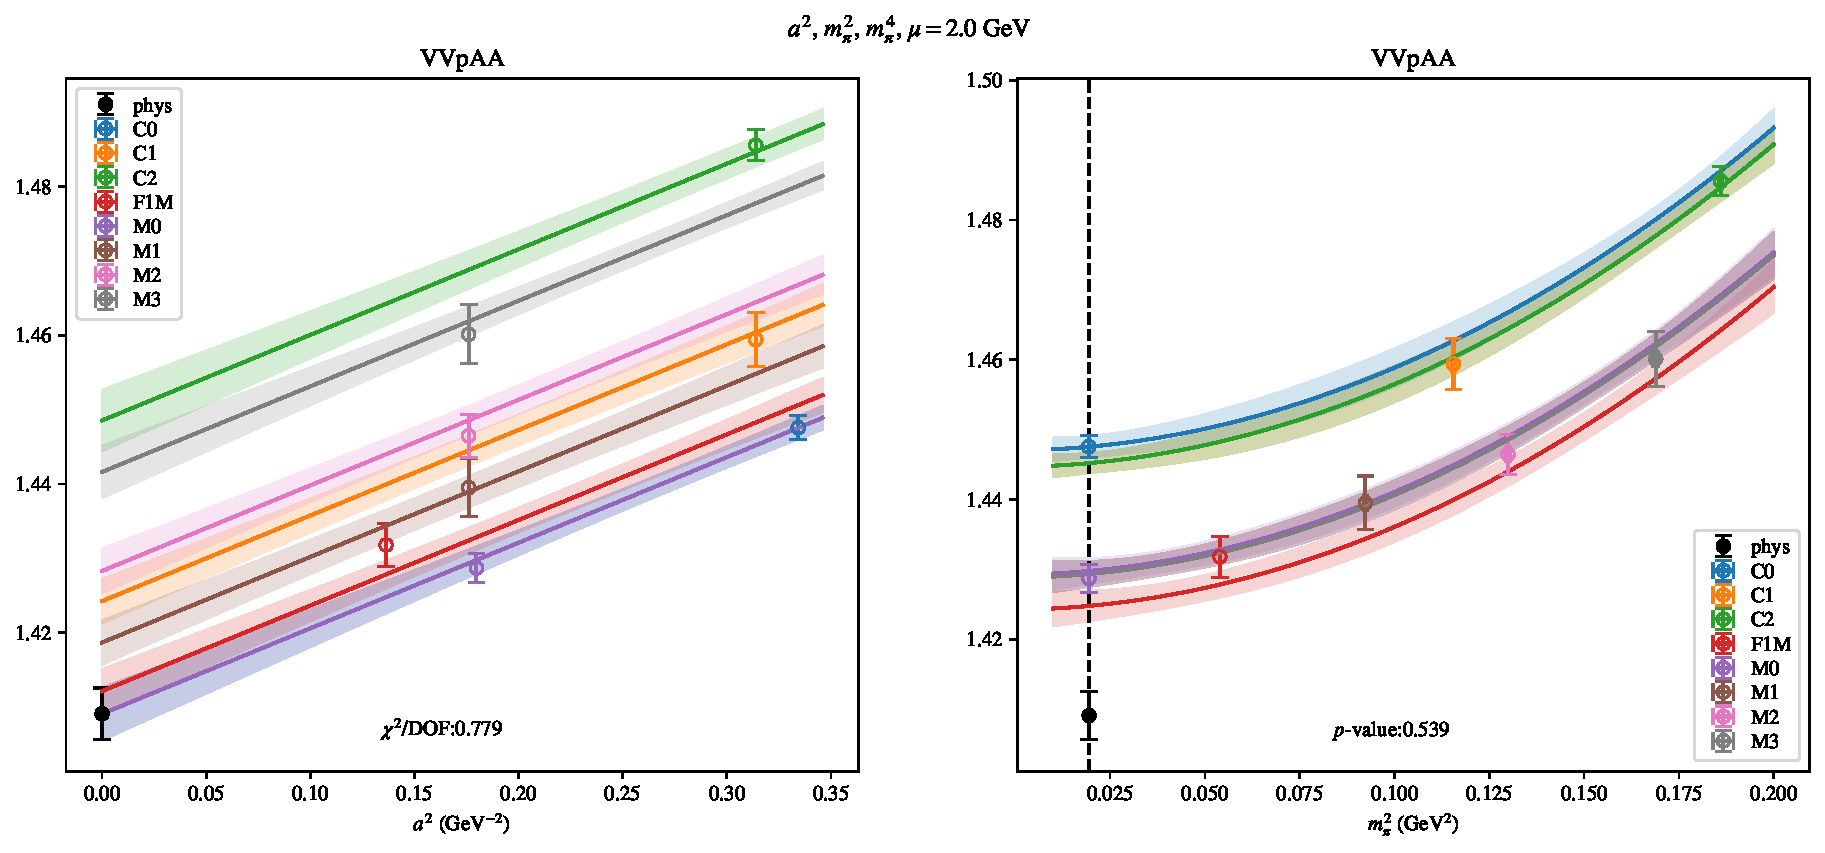
\includepdf[link, pages=-]{VVpAA/NPR/a2m2m4_20.pdf}
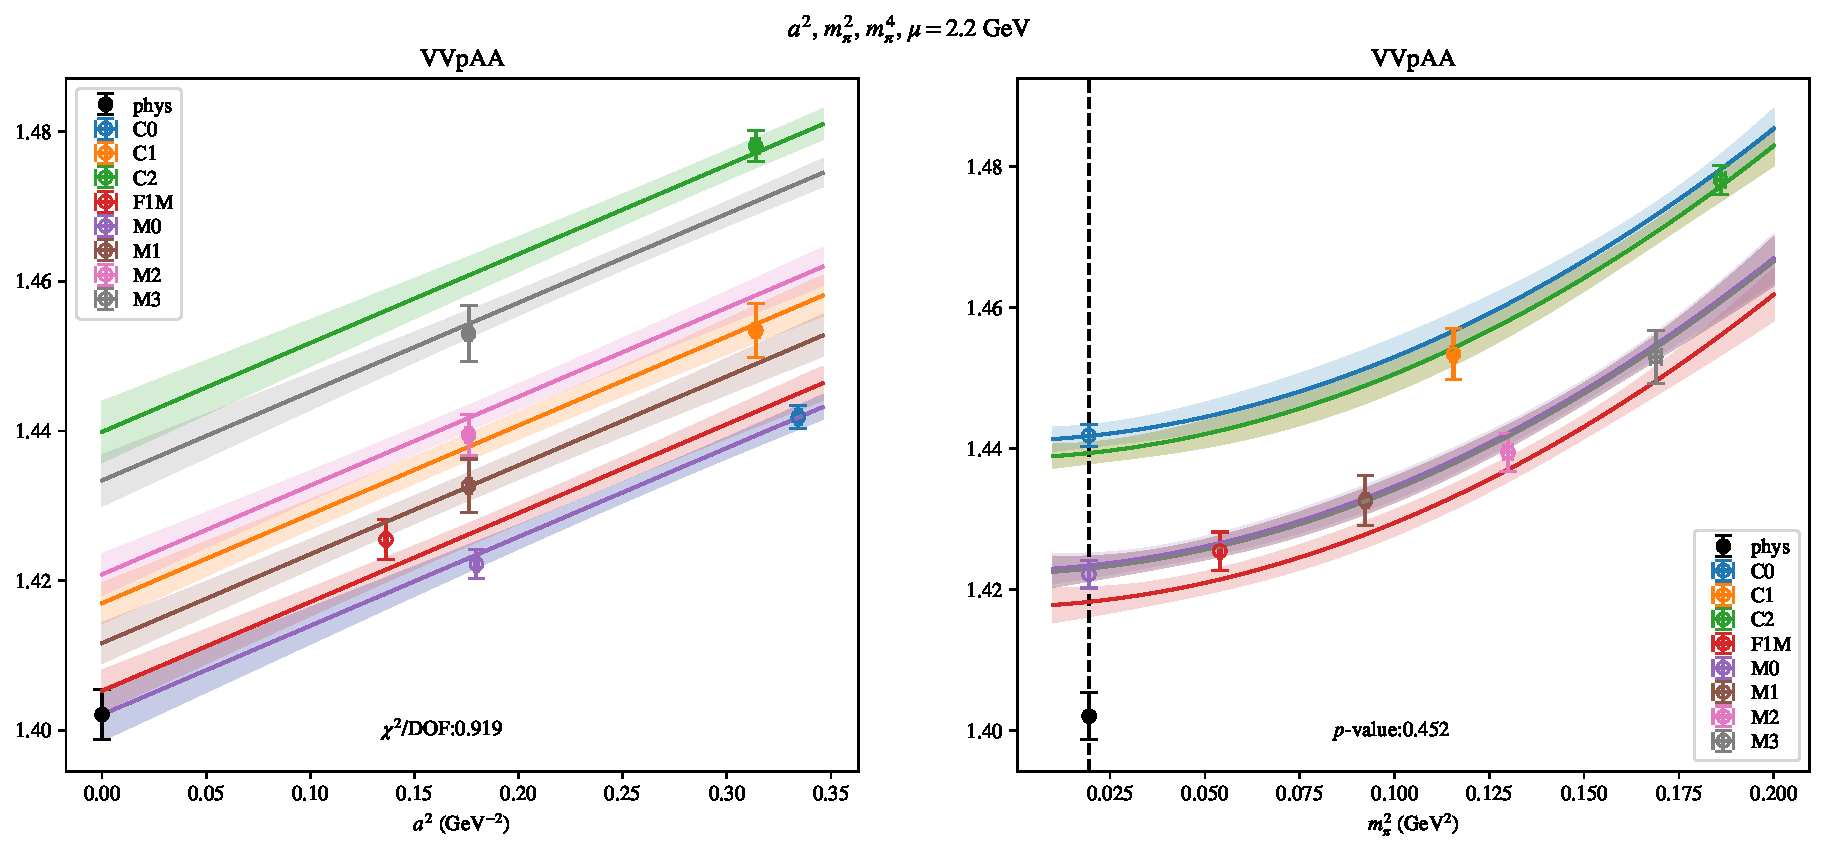
\includepdf[link, pages=-]{VVpAA/NPR/a2m2m4_22.pdf}
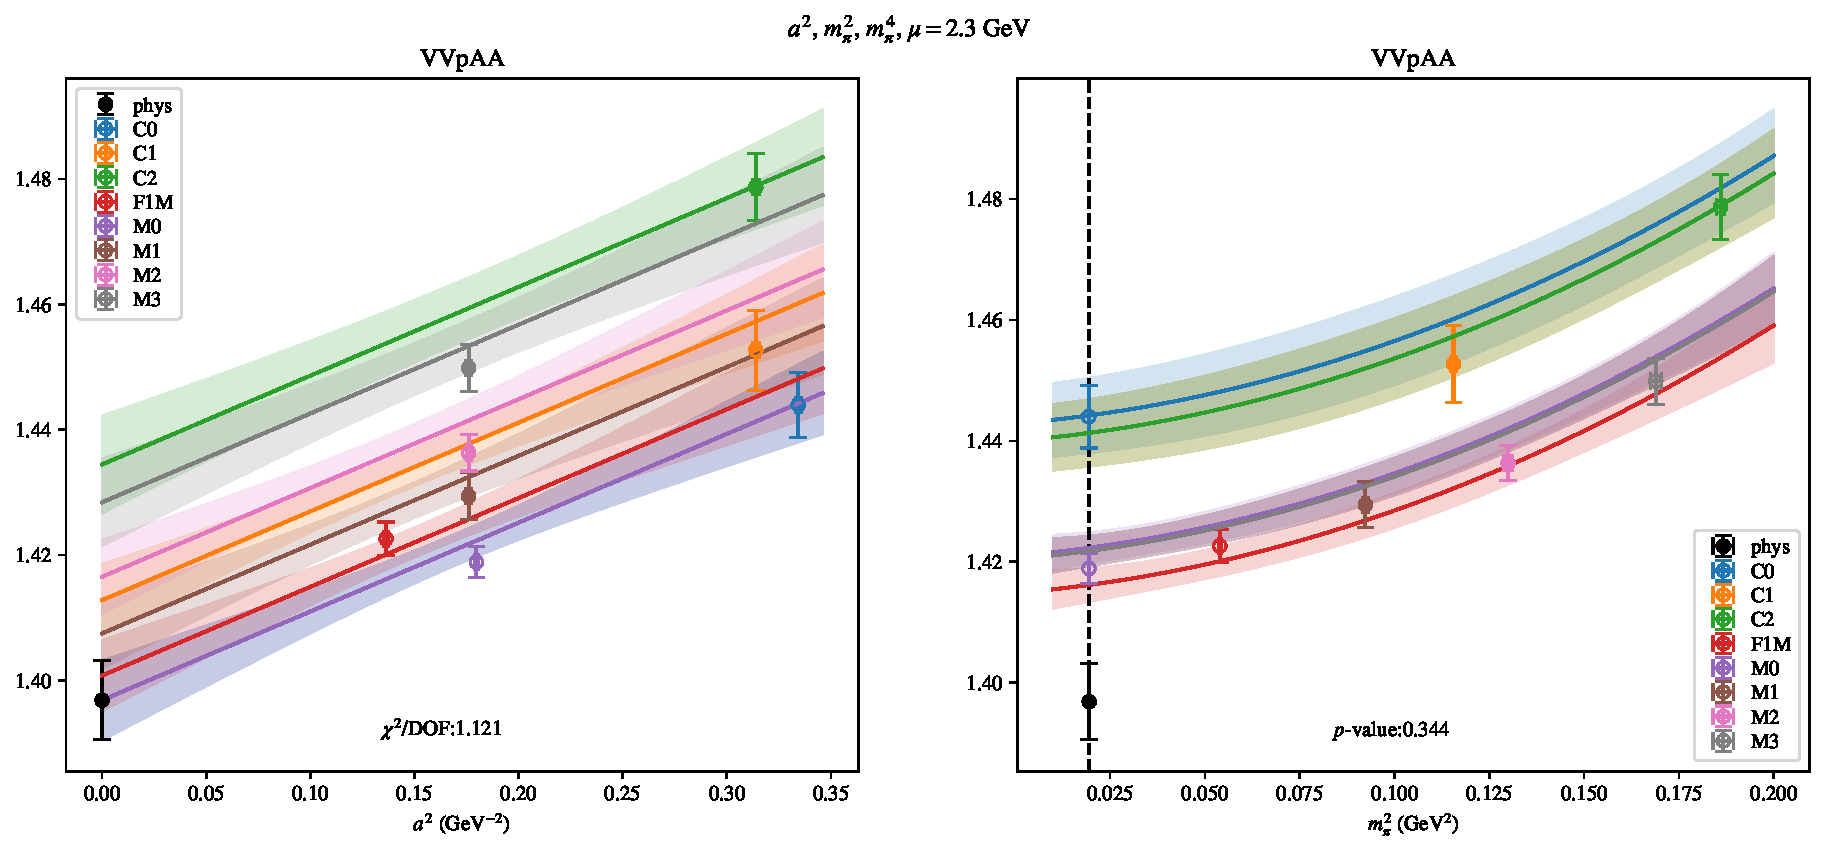
\includepdf[link, pages=-]{VVpAA/NPR/a2m2m4_23.pdf}
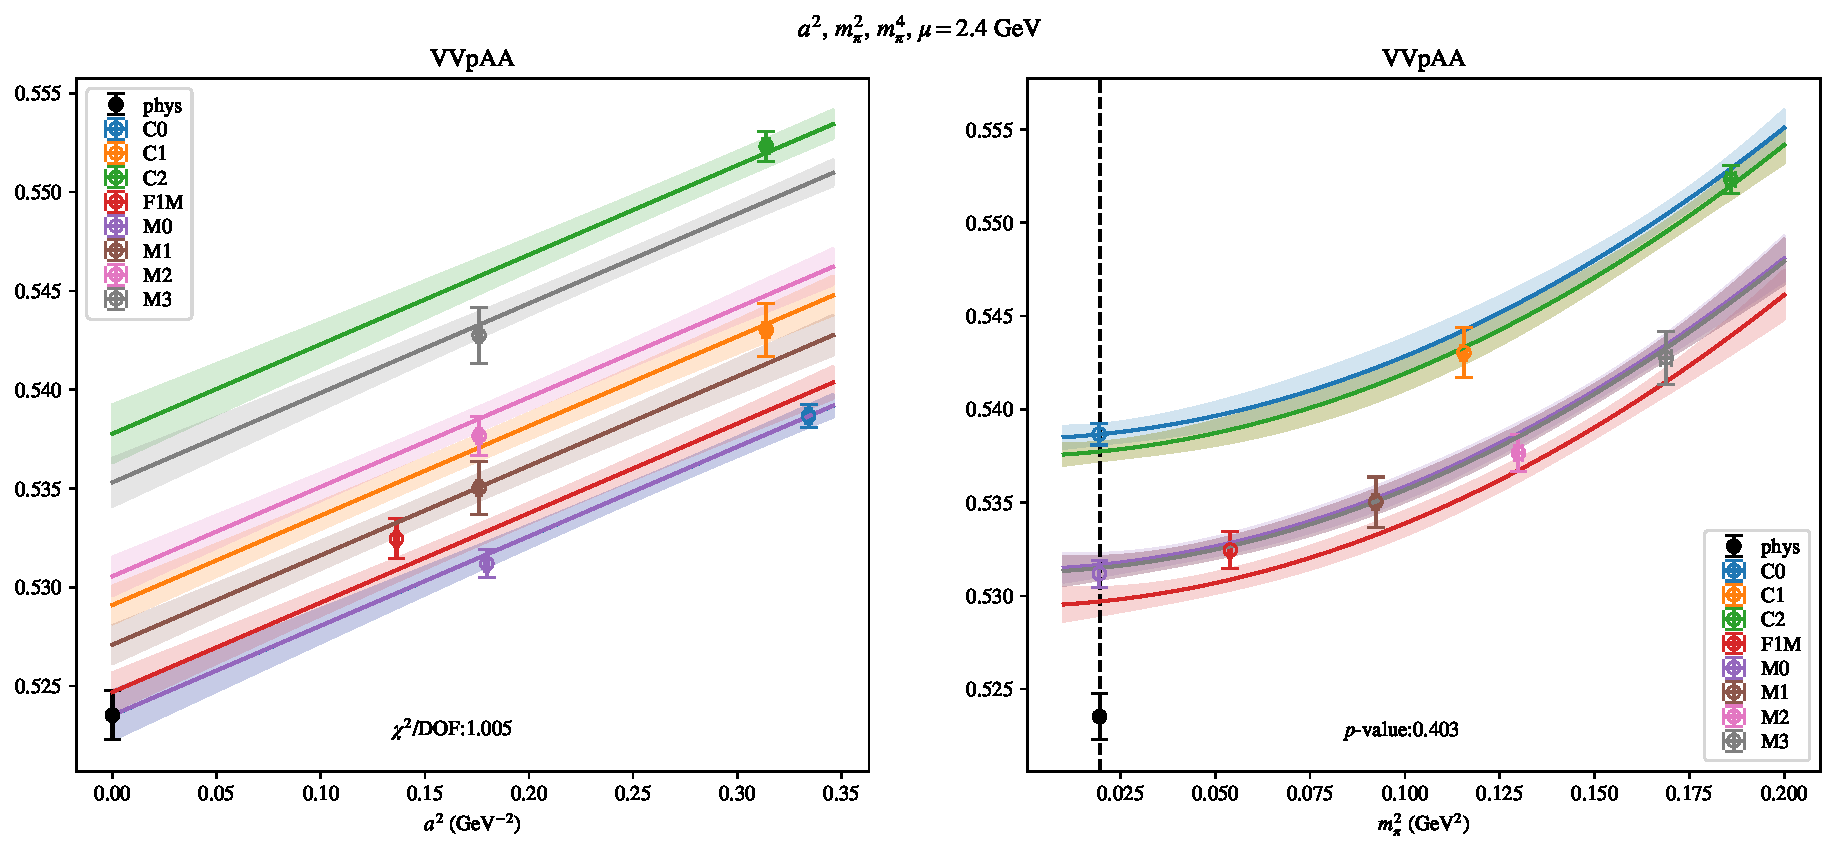
\includepdf[link, pages=-]{VVpAA/NPR/a2m2m4_24.pdf}
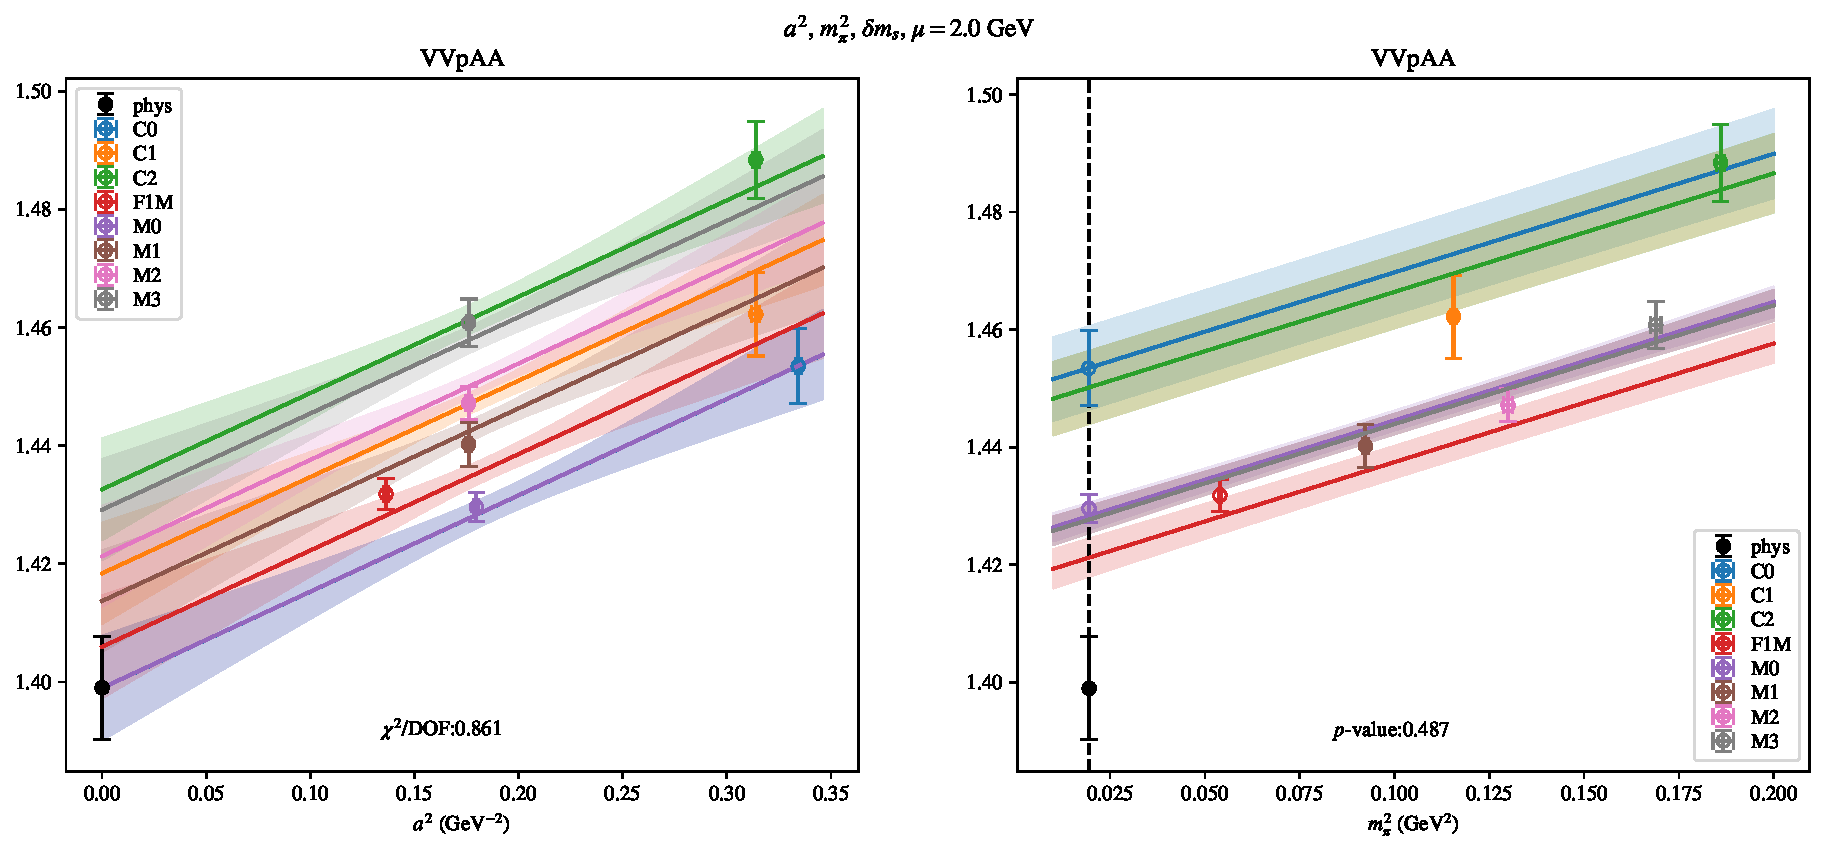
\includepdf[link, pages=-]{VVpAA/NPR/a2m2delm_20.pdf}
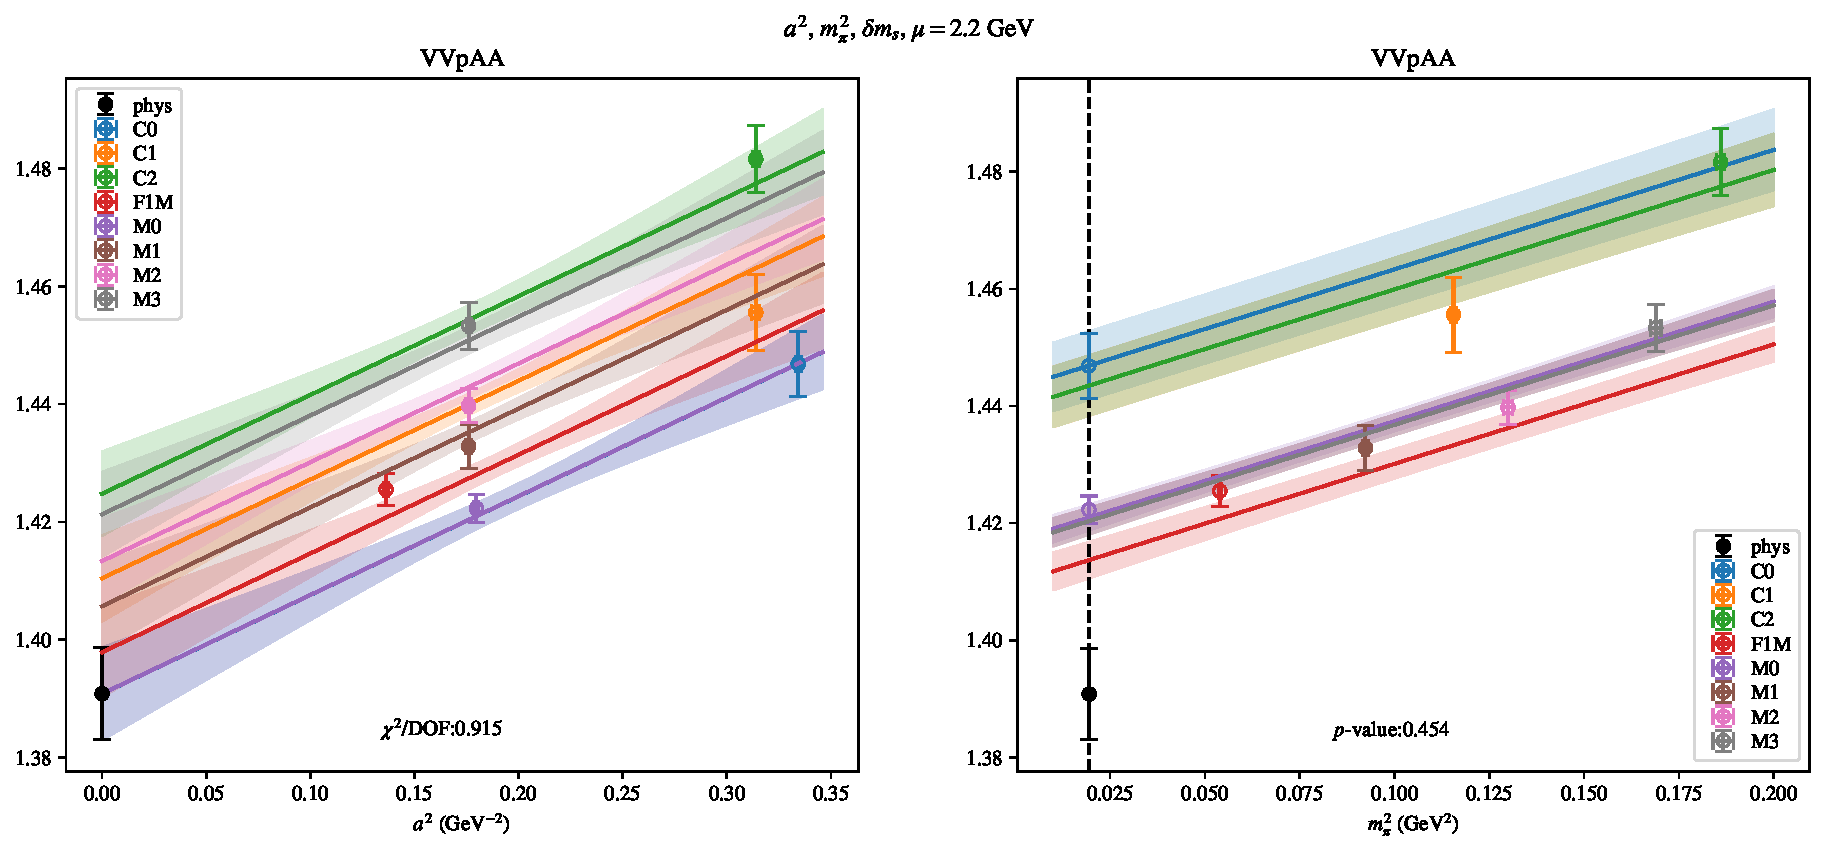
\includepdf[link, pages=-]{VVpAA/NPR/a2m2delm_22.pdf}
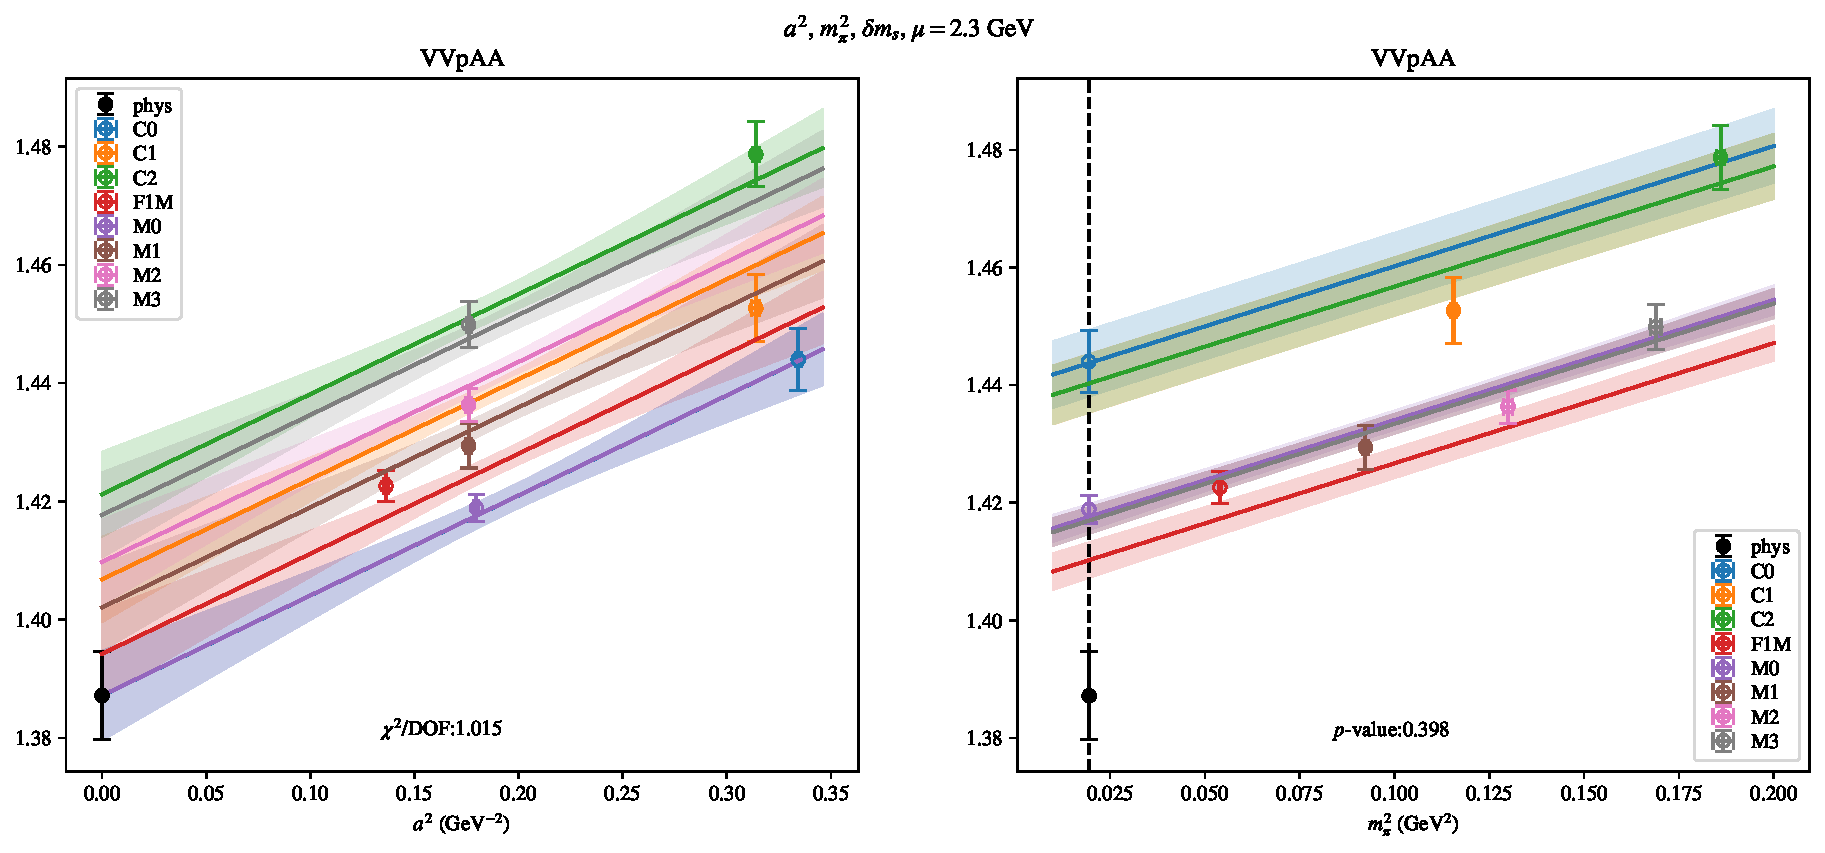
\includepdf[link, pages=-]{VVpAA/NPR/a2m2delm_23.pdf}
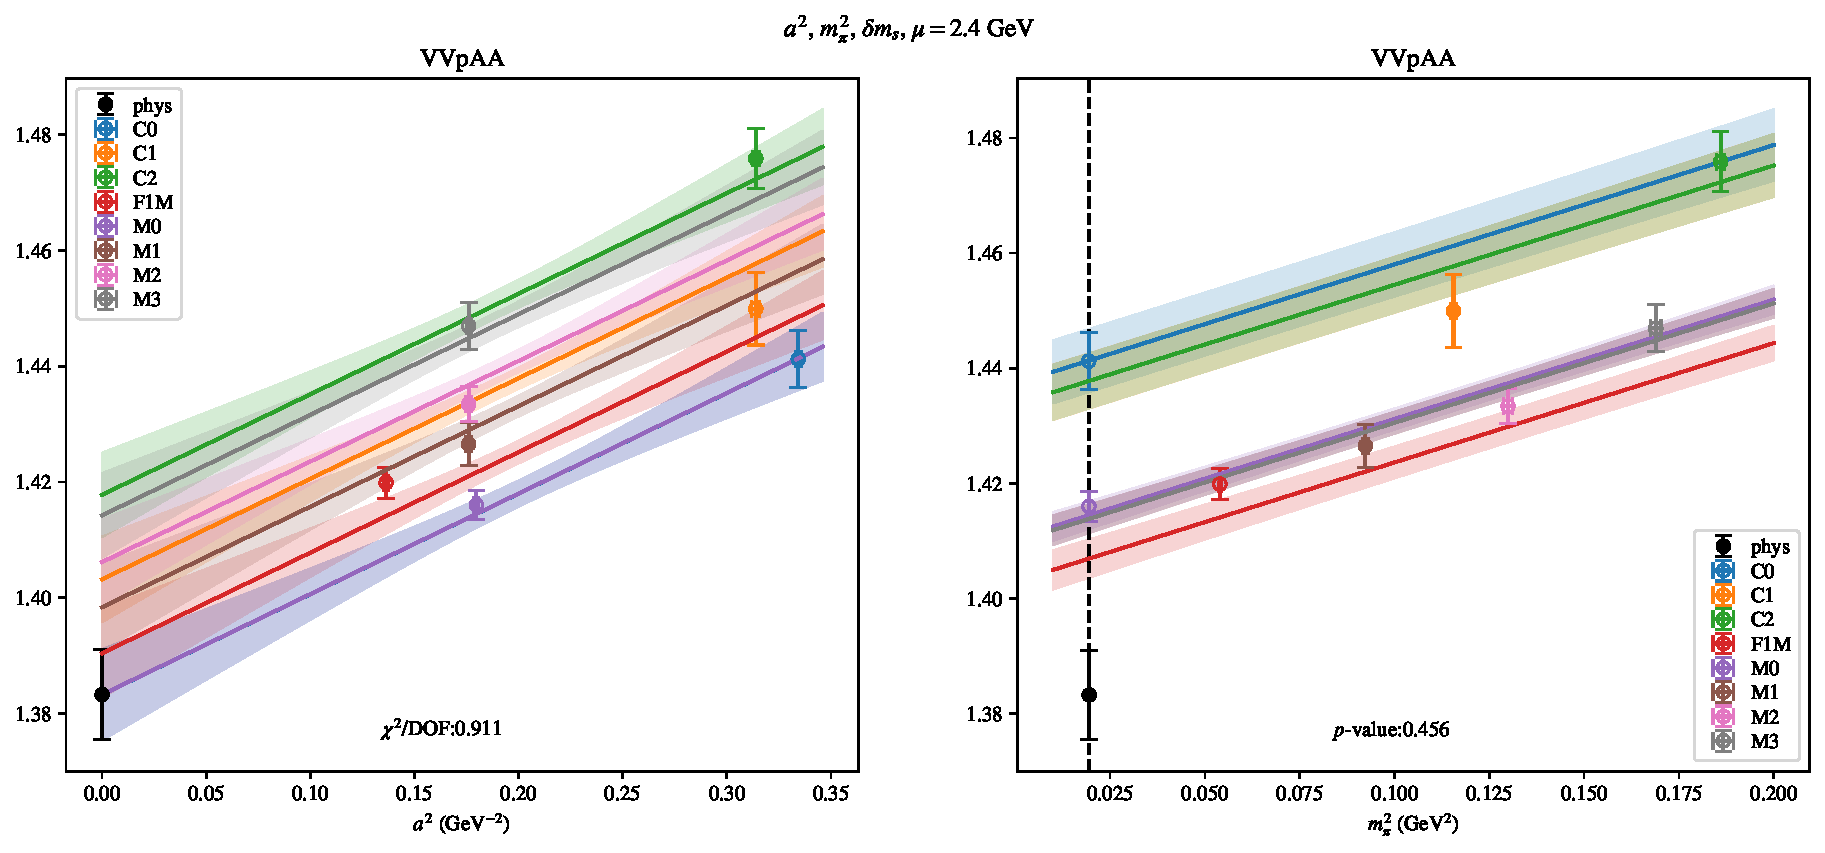
\includepdf[link, pages=-]{VVpAA/NPR/a2m2delm_24.pdf}
\clearpage
\section{$\mathcal{B}_2$}
\begin{table}[h!]
\begin{center}
\begin{tabular}{|c|c|c|c|c|c|c|}
\hline
$\mu$ (GeV) & $a^2$, $m_\pi^2$& $a^2$, $m_\pi^2$ (no C)& $a^2$, $a^4$, $m_\pi^2$& $a^2$, $m_\pi^2$ (no M3, C2)& $a^2$, $m_\pi^2$, $m_\pi^4$& $a^2$, $m_\pi^2$, $\delta m_s$\\
\hline
2.0& \hyperlink{VVmAA/NPR/a2m2_20.pdf.1}{\textbf{-0.96(27)}: 0.055 (0.998)} & \hyperlink{VVmAA/NPR/a2m2noC_20.pdf.1}{\textbf{-0.92(15)}: 0.472 (0.624)} & \hyperlink{VVmAA/NPR/a2a4m2_20.pdf.1}{\textbf{-0.8(37)}: 0.011 (1.0)} & \hyperlink{VVmAA/NPR/a2m2mcut_20.pdf.1}{\textbf{-0.96(32)}: 0.063 (0.979)} & \hyperlink{VVmAA/NPR/a2m2m4_20.pdf.1}{\textbf{-0.96(30)}: 0.072 (0.991)} & \hyperlink{VVmAA/NPR/a2m2delm_20.pdf.1}{\textbf{-0.9(12)}: 0.005 (1.0)}\\
2.2& \hyperlink{VVmAA/NPR/a2m2_22.pdf.1}{\textbf{-0.98(25)}: 0.055 (0.998)} & \hyperlink{VVmAA/NPR/a2m2noC_22.pdf.1}{\textbf{-0.95(12)}: 0.825 (0.438)} & \hyperlink{VVmAA/NPR/a2a4m2_22.pdf.1}{\textbf{-0.9(27)}: 0.013 (1.0)} & \hyperlink{VVmAA/NPR/a2m2mcut_22.pdf.1}{\textbf{-0.98(23)}: 0.065 (0.978)} & \hyperlink{VVmAA/NPR/a2m2m4_22.pdf.1}{\textbf{-0.98(23)}: 0.063 (0.993)} & \hyperlink{VVmAA/NPR/a2m2delm_22.pdf.1}{\textbf{-1.00(94)}: 0.008 (1.0)}\\
2.3& \hyperlink{VVmAA/NPR/a2m2_23.pdf.1}{\textbf{-0.98(22)}: 0.055 (0.998)} & \hyperlink{VVmAA/NPR/a2m2noC_23.pdf.1}{\textbf{-0.95(11)}: 1.177 (0.308)} & \hyperlink{VVmAA/NPR/a2a4m2_23.pdf.1}{\textbf{-0.9(21)}: 0.017 (0.999)} & \hyperlink{VVmAA/NPR/a2m2mcut_23.pdf.1}{\textbf{-0.98(25)}: 0.06 (0.981)} & \hyperlink{VVmAA/NPR/a2m2m4_23.pdf.1}{\textbf{-0.99(27)}: 0.058 (0.994)} & \hyperlink{VVmAA/NPR/a2m2delm_23.pdf.1}{\textbf{-1.00(83)}: 0.01 (1.0)}\\
2.4& \hyperlink{VVmAA/NPR/a2m2_24.pdf.1}{\textbf{-0.99(24)}: 0.08 (0.995)} & \hyperlink{VVmAA/NPR/a2m2noC_24.pdf.1}{\textbf{-0.96(10)}: 1.526 (0.217)} & \hyperlink{VVmAA/NPR/a2a4m2_24.pdf.1}{\textbf{-0.9(20)}: 0.02 (0.999)} & \hyperlink{VVmAA/NPR/a2m2mcut_24.pdf.1}{\textbf{-0.99(26)}: 0.075 (0.973)} & \hyperlink{VVmAA/NPR/a2m2m4_24.pdf.1}{\textbf{-0.99(24)}: 0.091 (0.985)} & \hyperlink{VVmAA/NPR/a2m2delm_24.pdf.1}{\textbf{-1.01(71)}: 0.014 (1.0)}\\
\hline
\end{tabular}
\caption{Physical point value from chiral and continuum extrapolation at renormalisation scale $\mu$. Entries are \textbf{value(error)}: $\chi^2/\text{DOF}$ ($p$-value).}
\end{center}
\end{table}
\begin{table}[h!]
\begin{center}
\begin{tabular}{|c c|c|c|c|c|c|c|}
\hline
$\mu$ (GeV) &  & $a^2$, $m_\pi^2$& $a^2$, $m_\pi^2$ (no C)& $a^2$, $a^4$, $m_\pi^2$& $a^2$, $m_\pi^2$ (no M3, C2)& $a^2$, $m_\pi^2$, $m_\pi^4$& $a^2$, $m_\pi^2$, $\delta m_s$\\
\hline
\multirow{2}{0.5in}{2.0} & $\alpha$ & -0.1& 0.24(12)& 1.147& -0.086& -0.1(21)& -0.1(52)\\
 & $\beta$ & 0.0026(29)& 0.00228(24)& 0.0014(74)& 0.0026(41)& 0.0& 0.0013(23)\\
\hline
\multirow{2}{0.5in}{2.2} & $\alpha$ & -0.1(18)& 0.069(89)& 0.617& -0.1(16)& -0.1(16)& -0.2(35)\\
 & $\beta$ & 0.0023(26)& 0.00191(22)& 0.0014(17)& 0.0020(29)& -0.0& 0.0013(14)\\
\hline
\multirow{2}{0.5in}{2.3} & $\alpha$ & -0.1(16)& 0.051(77)& 0.577& -0.1(16)& -0.1(18)& -0.2(31)\\
 & $\beta$ & 0.0021(23)& 0.00180(21)& 0.00145(84)& 0.0019(30)& -0.001& 0.0012(12)\\
\hline
\multirow{2}{0.5in}{2.4} & $\alpha$ & -0.1(17)& 0.028(68)& 0.542& -0.1(17)& -0.2(16)& -0.2(28)\\
 & $\beta$ & 0.0023(23)& 0.00170(20)& 0.00139(60)& 0.0019(29)& -0.001& 0.00124(99)\\
\hline
\end{tabular}
\caption{Fit values of coefficients in $Q = Q_{phys} + \mathbf{\alpha} a^2 + \mathbf{\beta}\left(\frac{m_\pi^2}{f_\pi^2}-\frac{m_{\pi,PDG}^2}{f_\pi^2}\right) + \ldots$.}
\end{center}
\end{table}
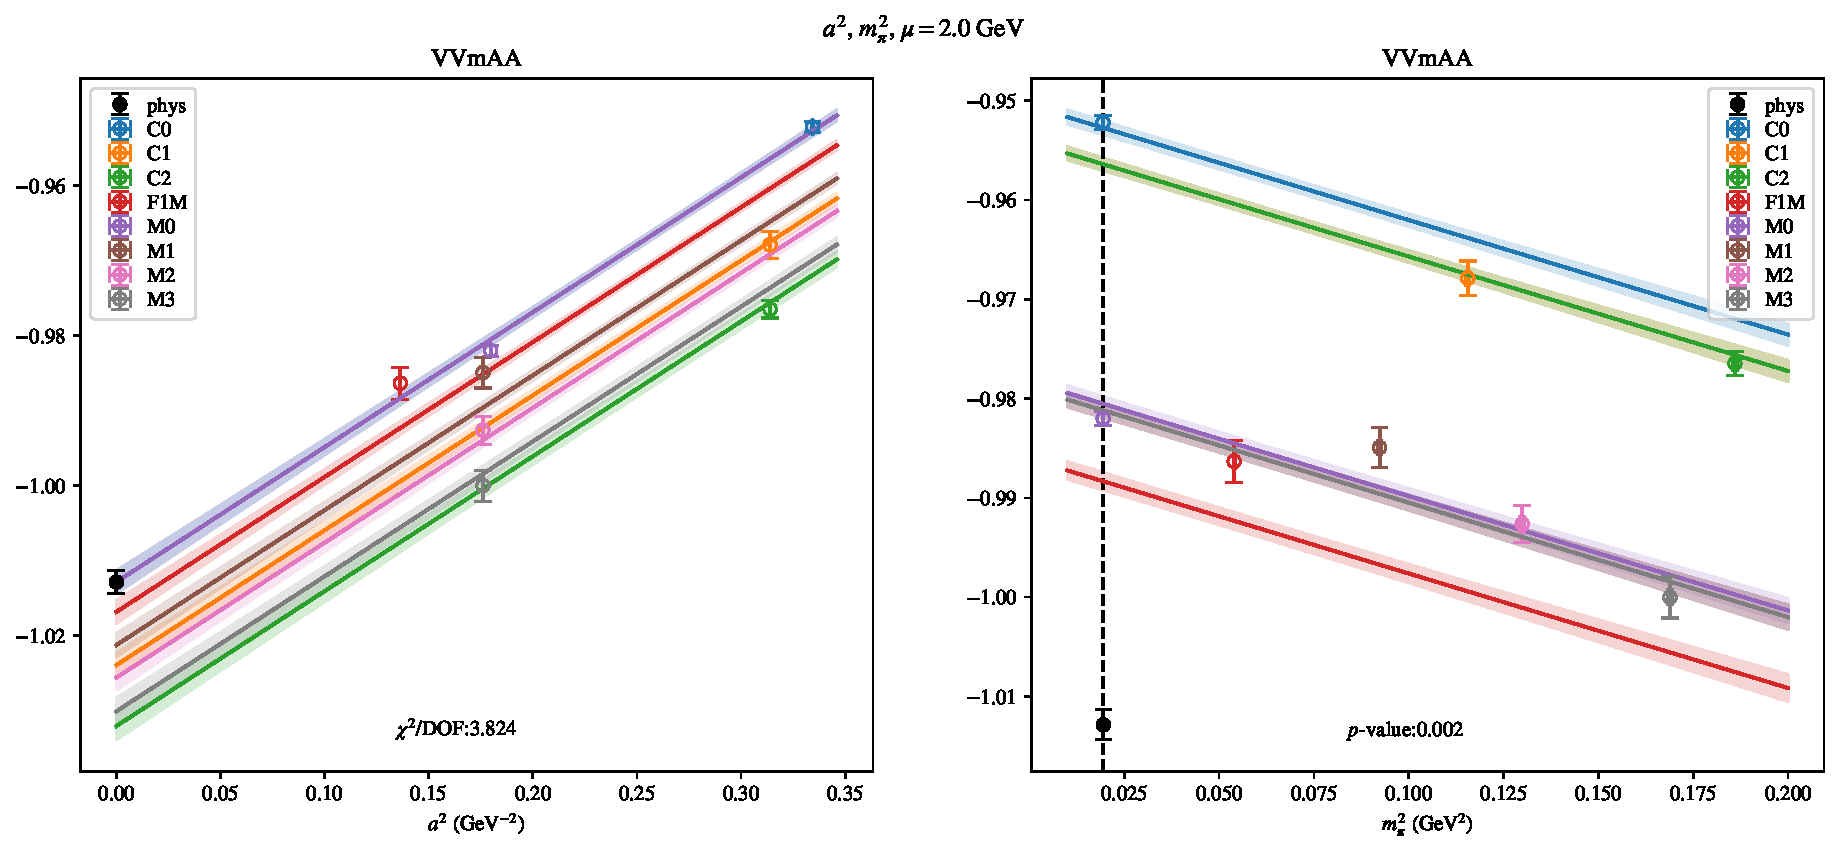
\includepdf[link, pages=-]{VVmAA/NPR/a2m2_20.pdf}
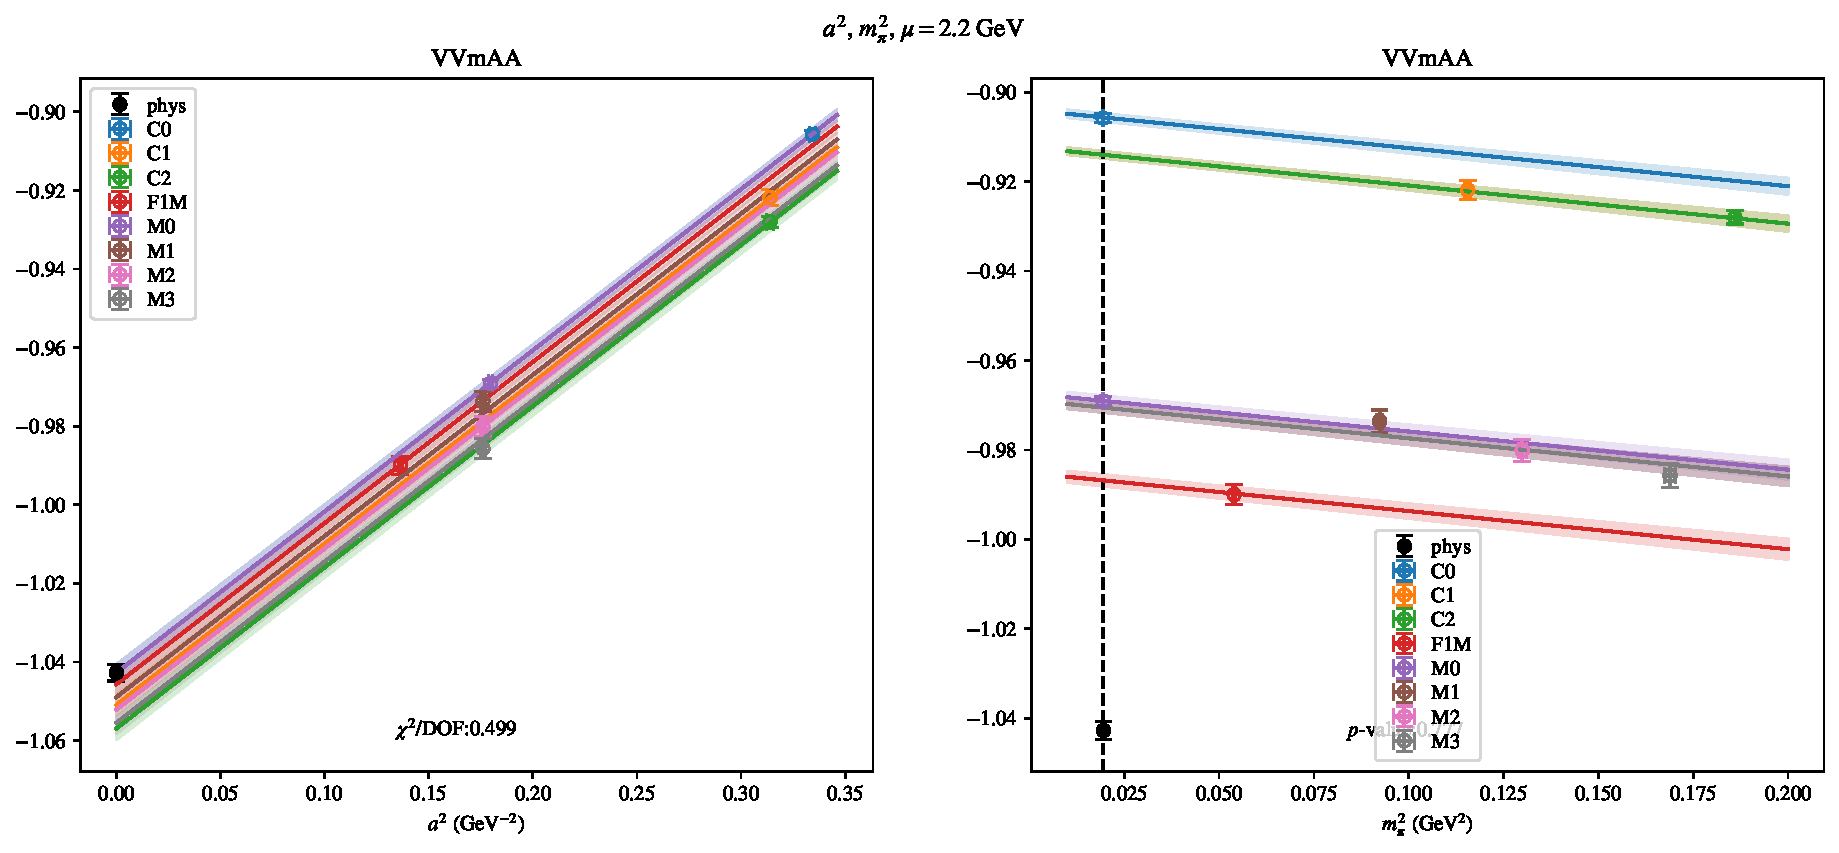
\includepdf[link, pages=-]{VVmAA/NPR/a2m2_22.pdf}
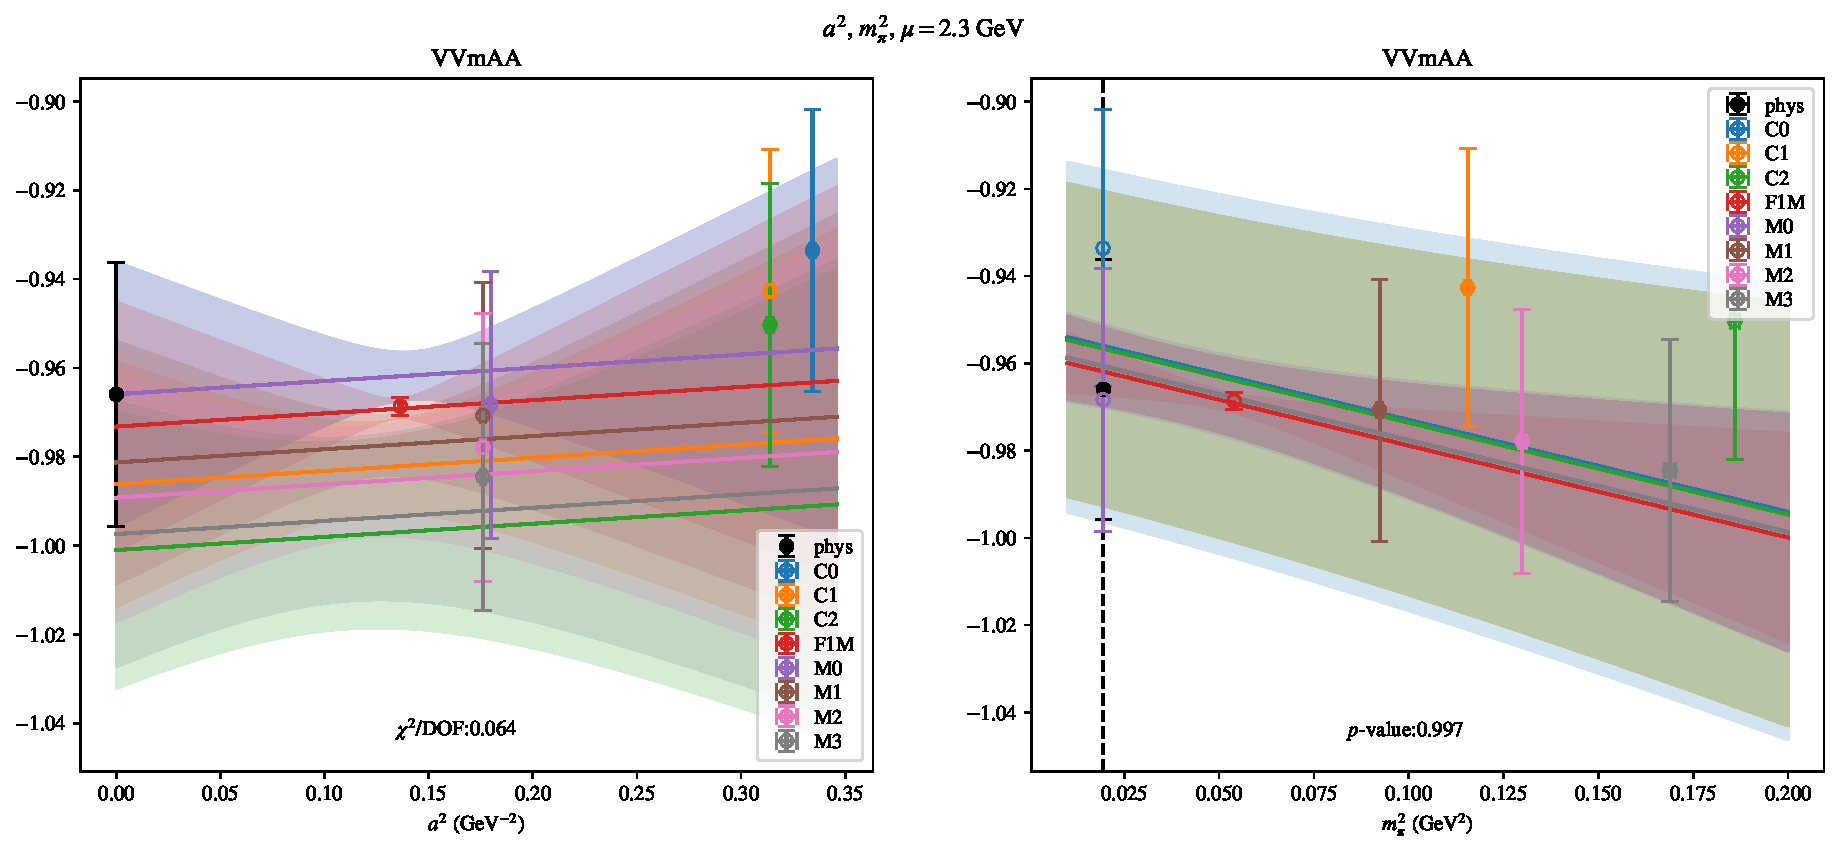
\includepdf[link, pages=-]{VVmAA/NPR/a2m2_23.pdf}
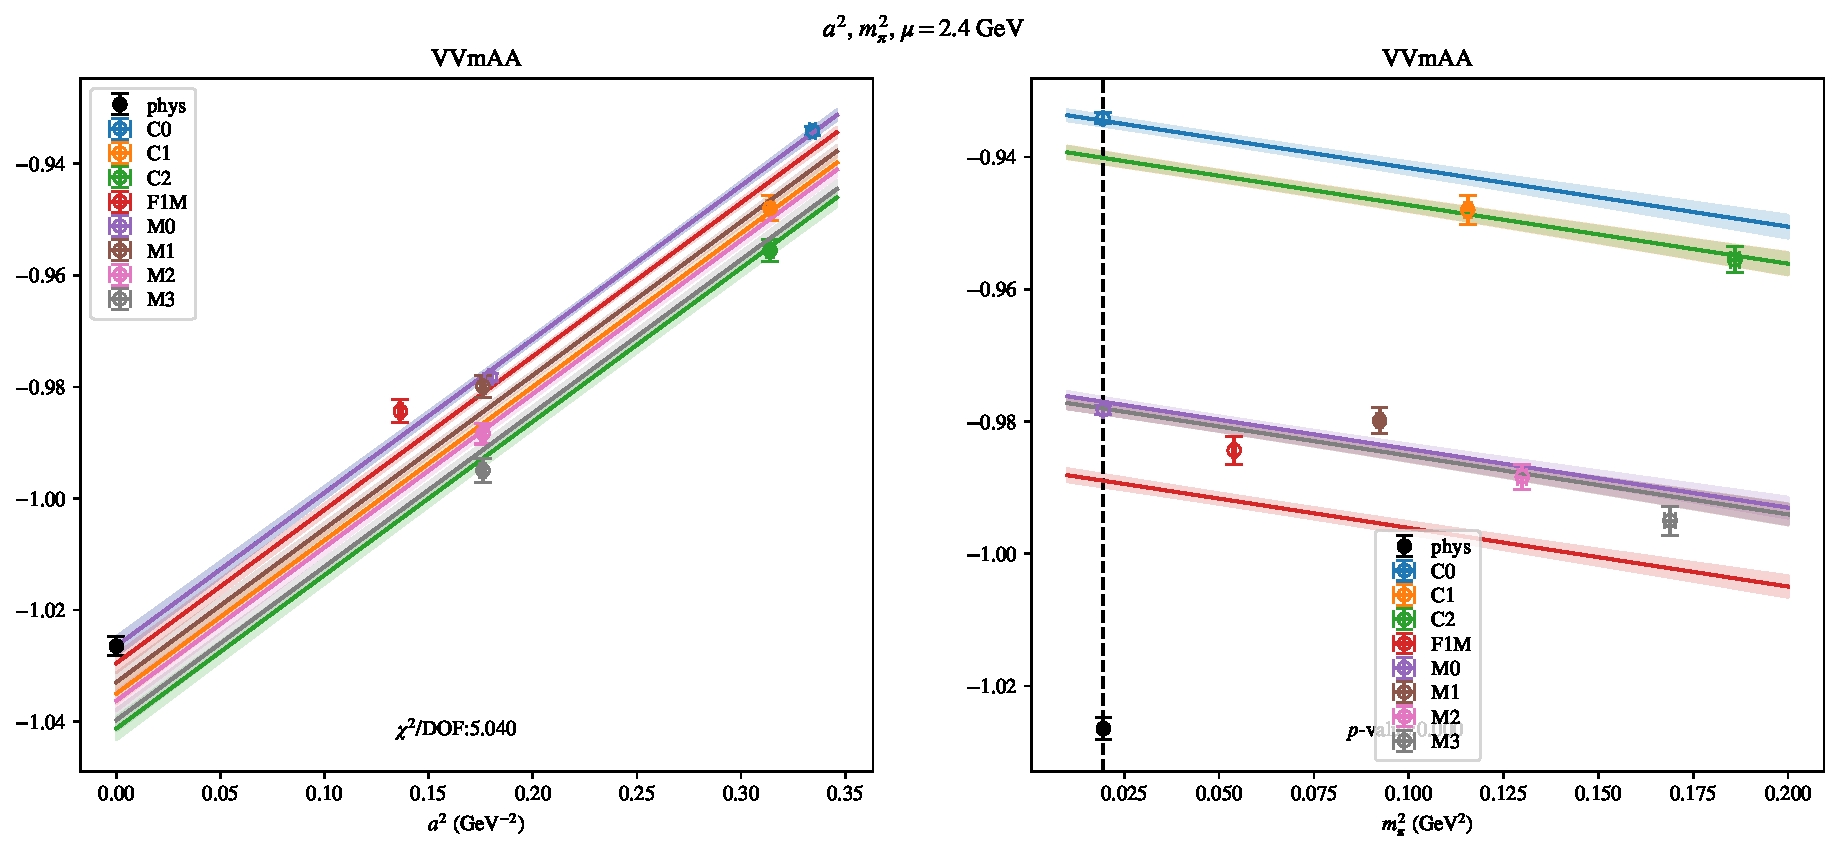
\includepdf[link, pages=-]{VVmAA/NPR/a2m2_24.pdf}
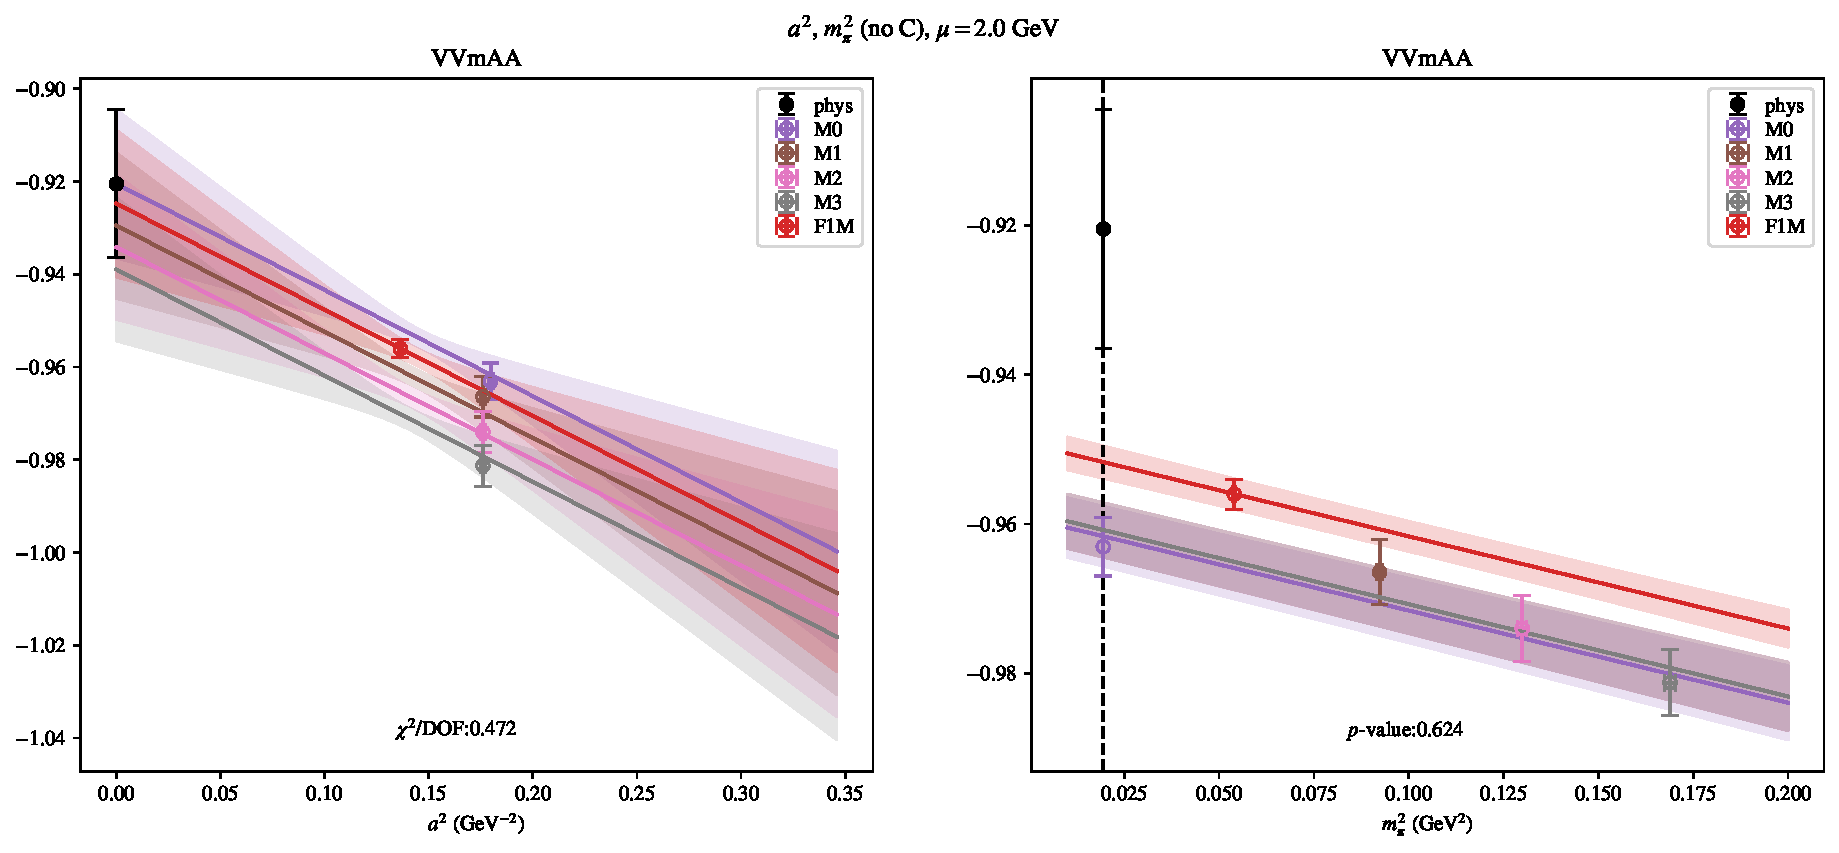
\includepdf[link, pages=-]{VVmAA/NPR/a2m2noC_20.pdf}
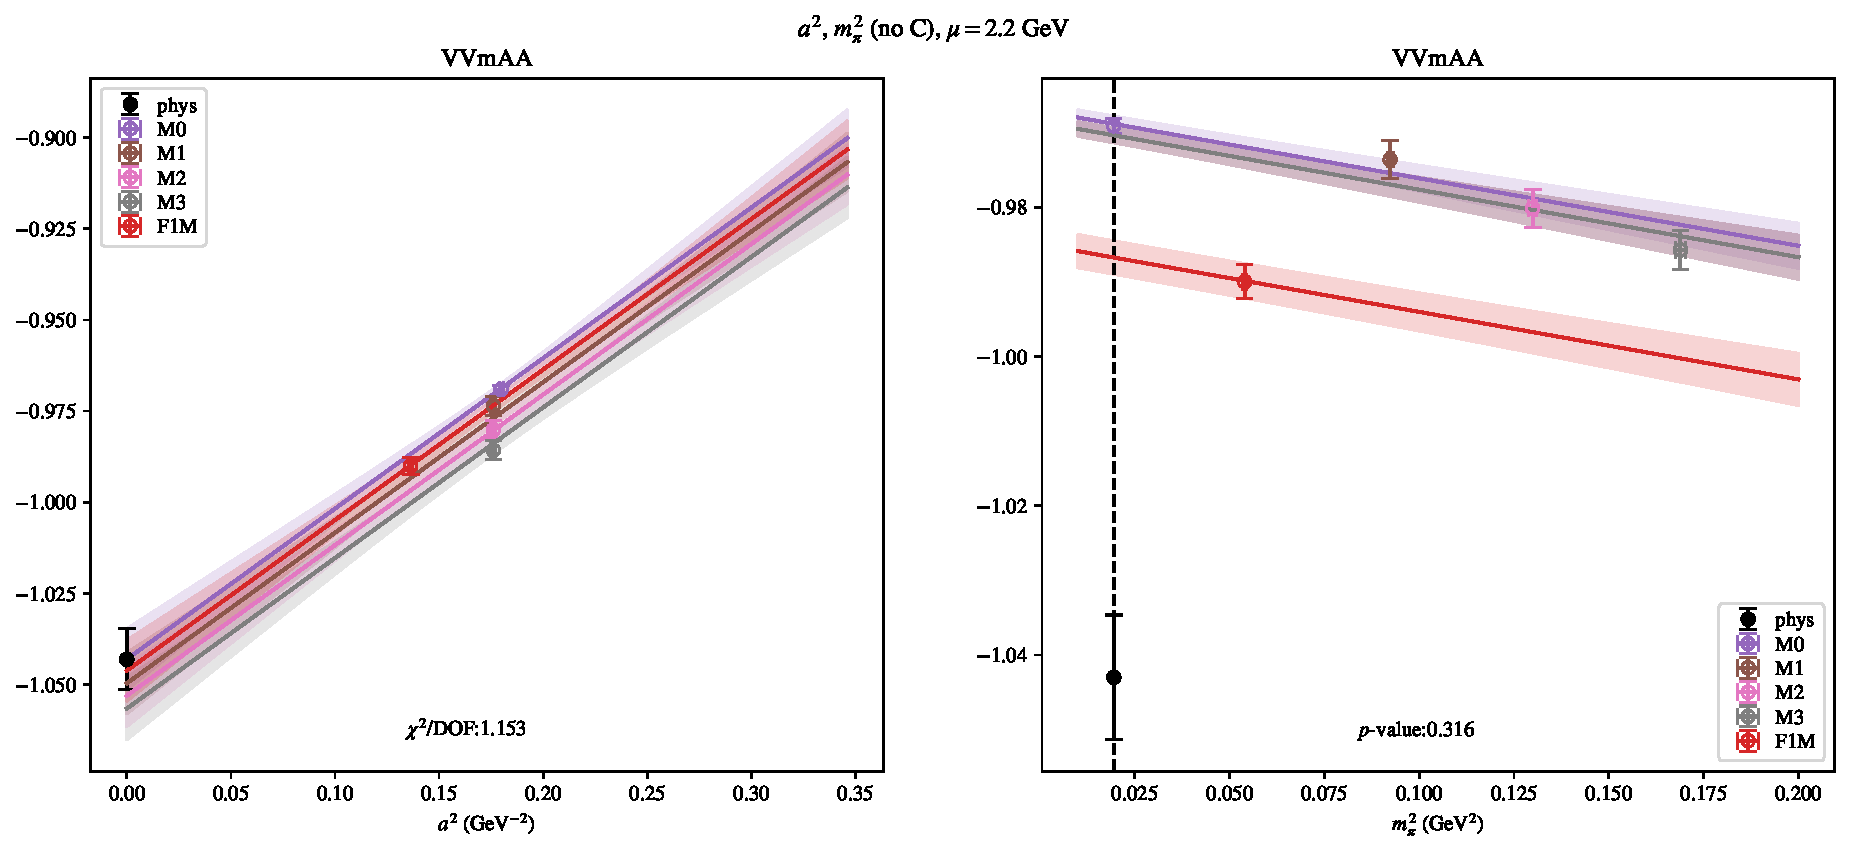
\includepdf[link, pages=-]{VVmAA/NPR/a2m2noC_22.pdf}
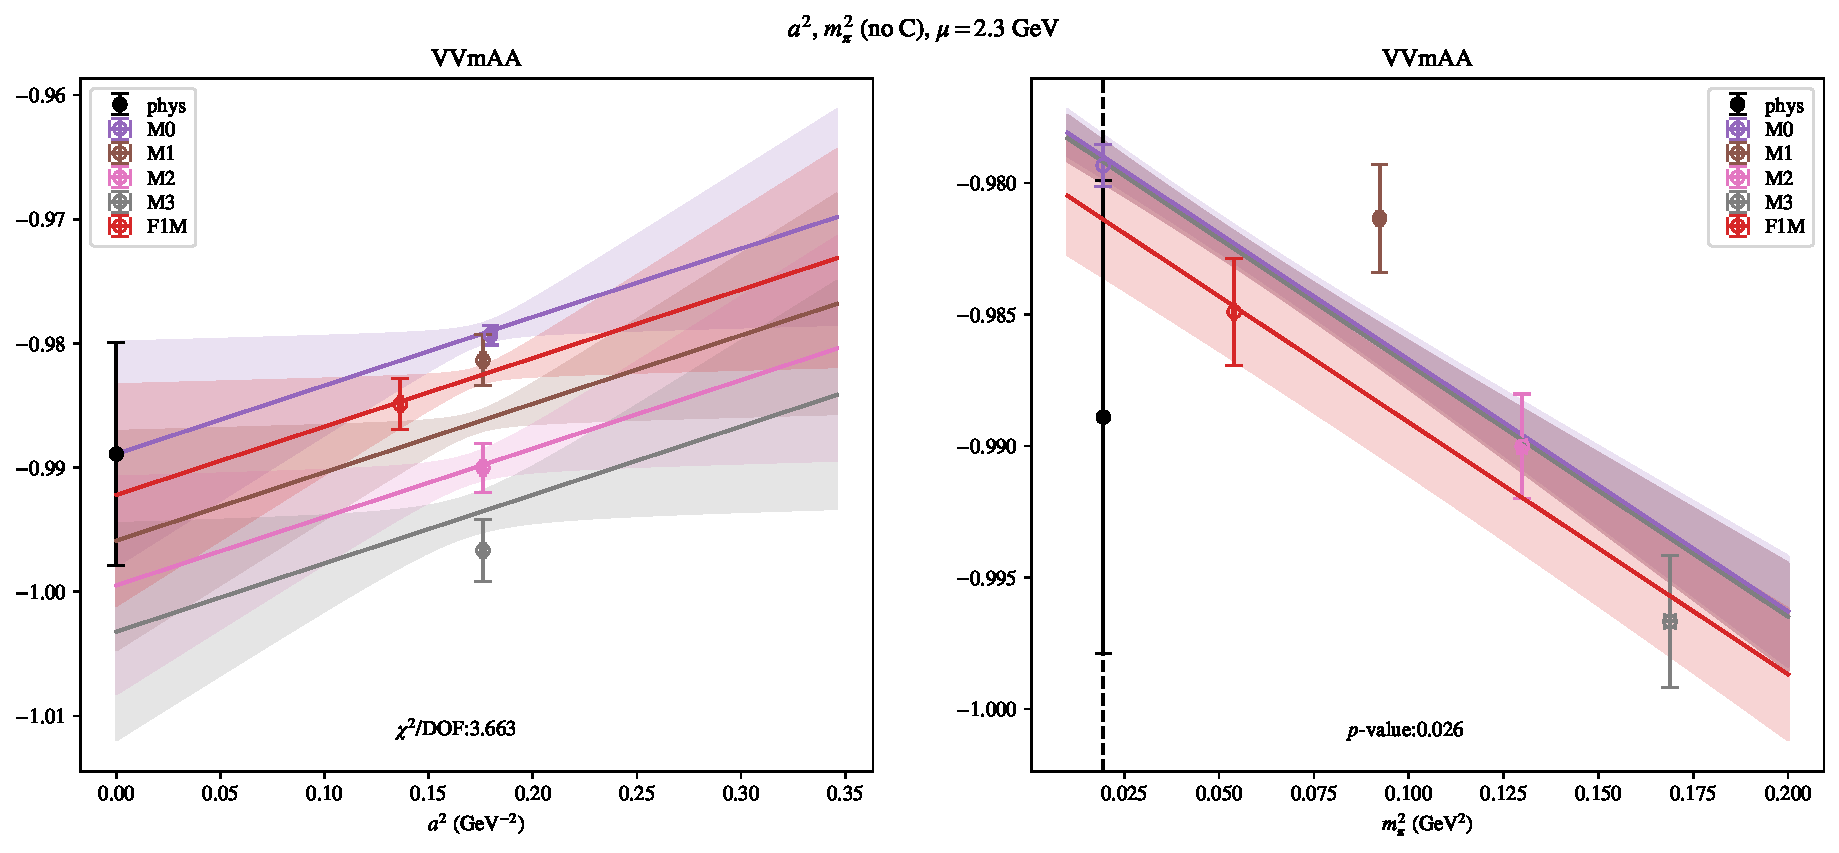
\includepdf[link, pages=-]{VVmAA/NPR/a2m2noC_23.pdf}
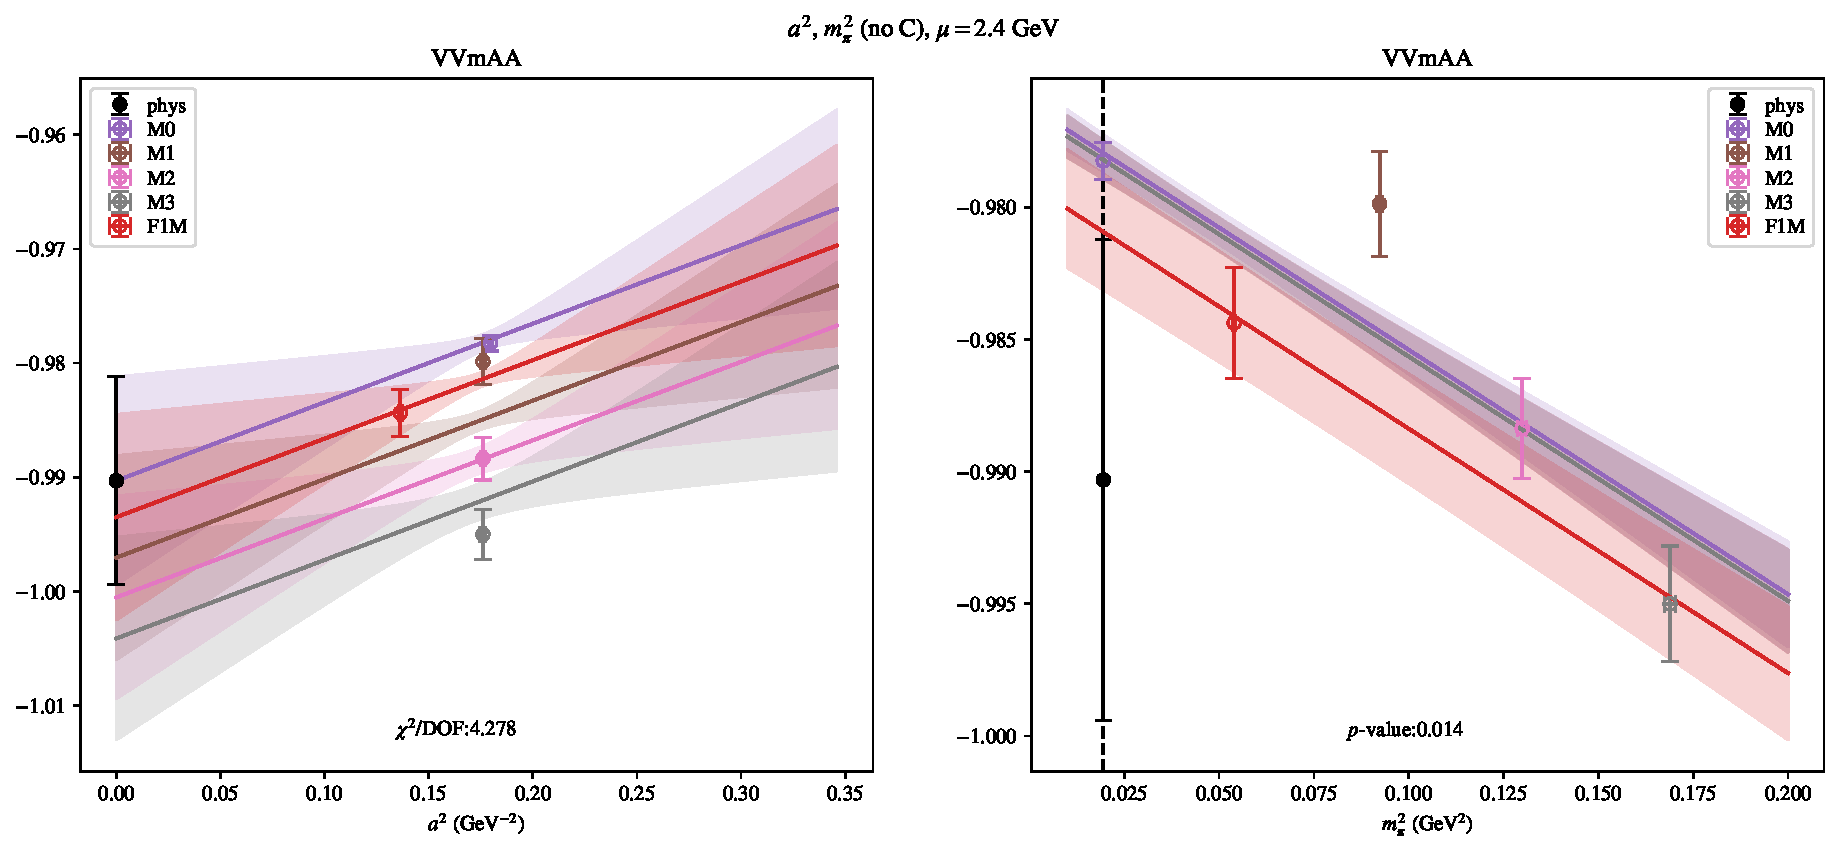
\includepdf[link, pages=-]{VVmAA/NPR/a2m2noC_24.pdf}
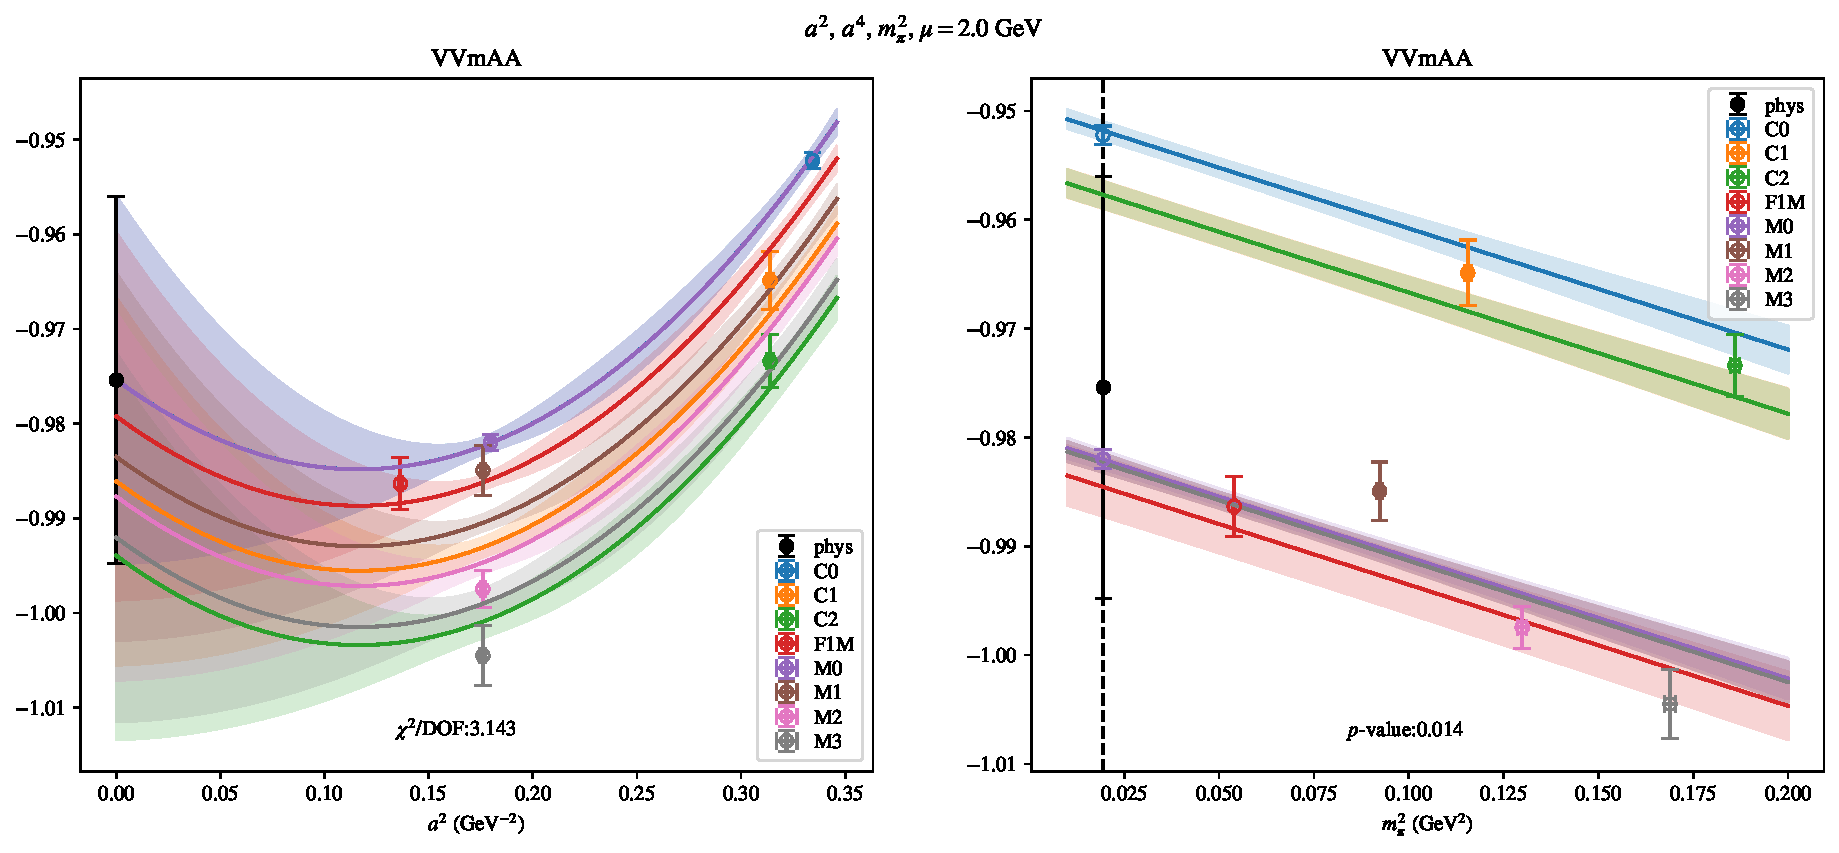
\includepdf[link, pages=-]{VVmAA/NPR/a2a4m2_20.pdf}
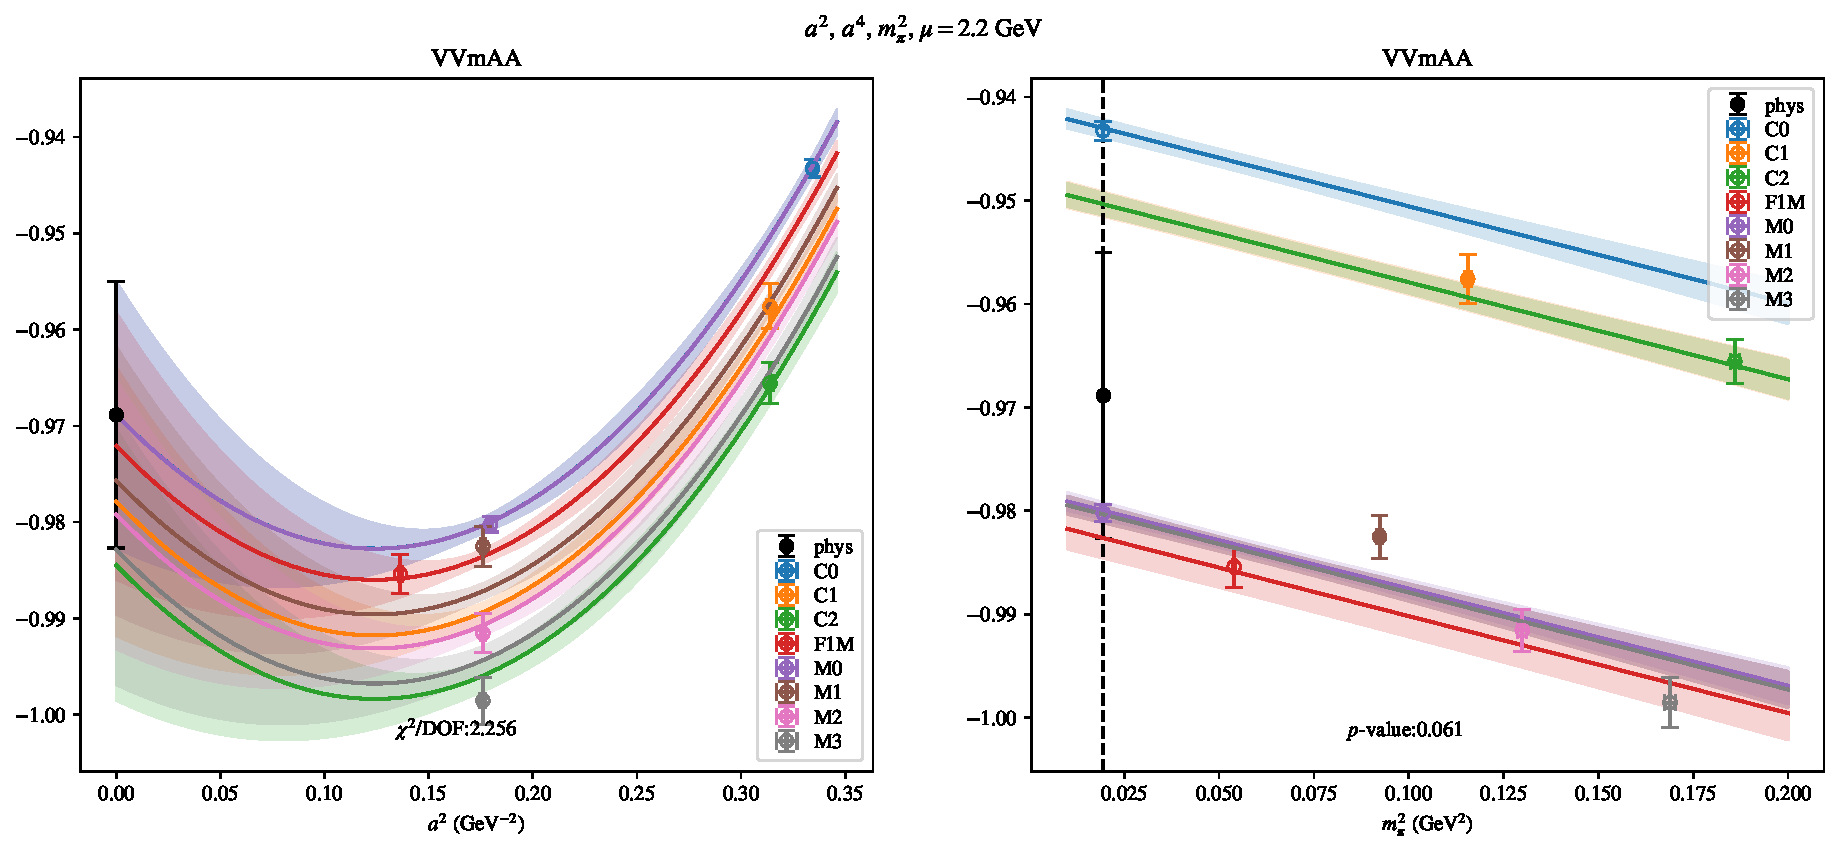
\includepdf[link, pages=-]{VVmAA/NPR/a2a4m2_22.pdf}
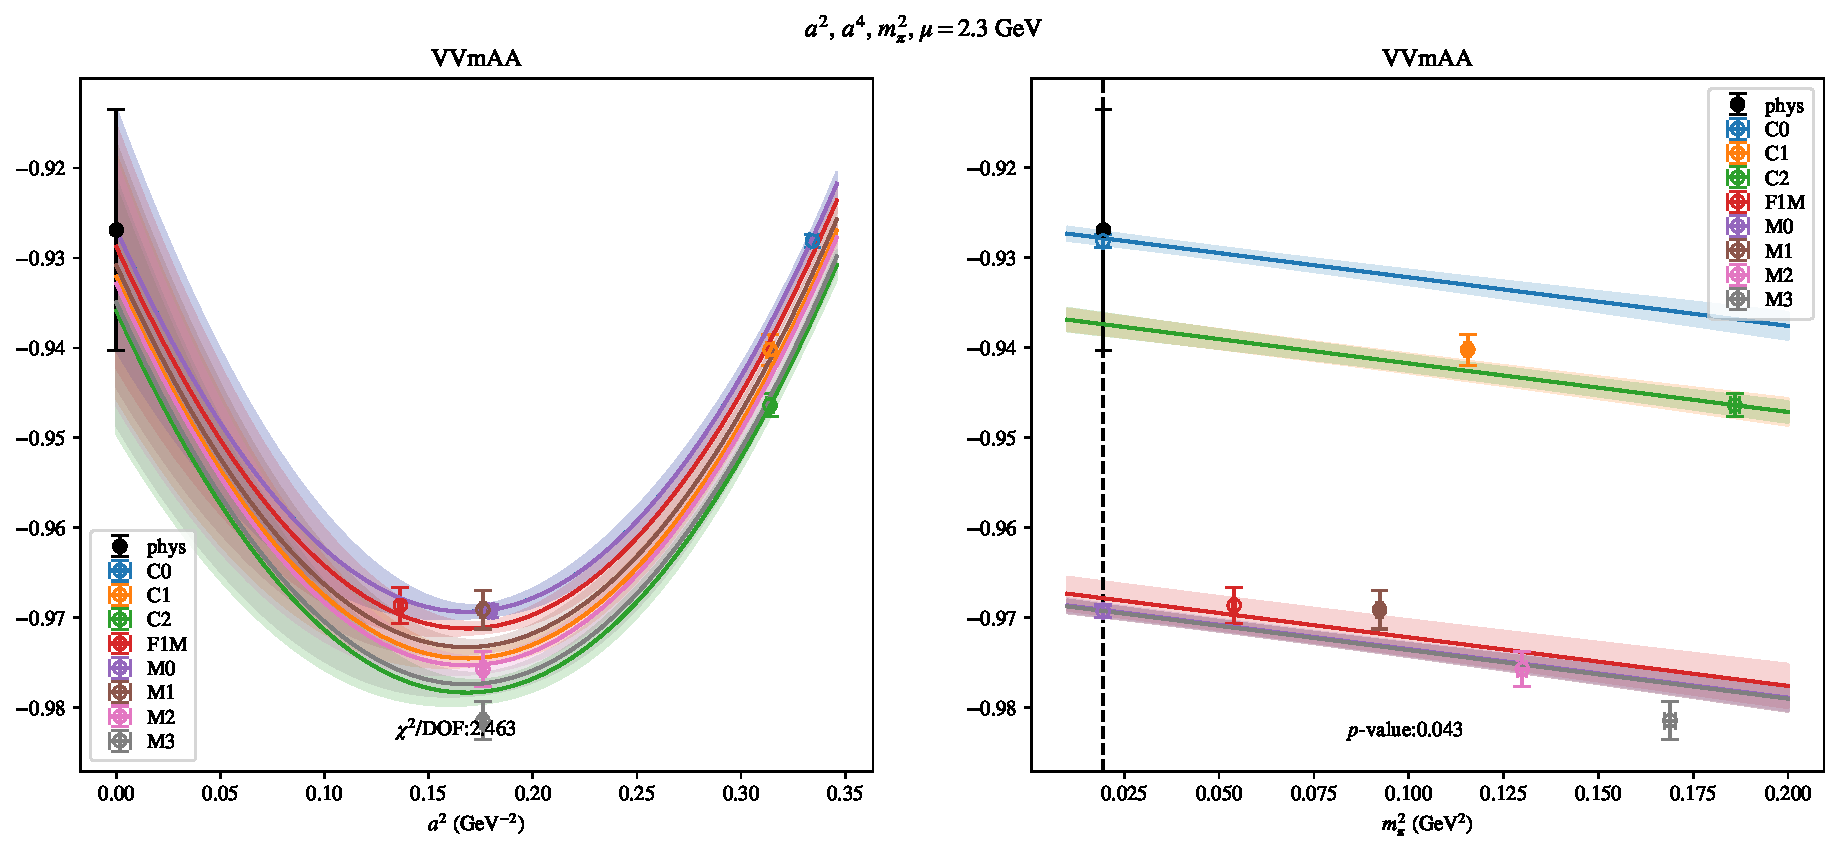
\includepdf[link, pages=-]{VVmAA/NPR/a2a4m2_23.pdf}
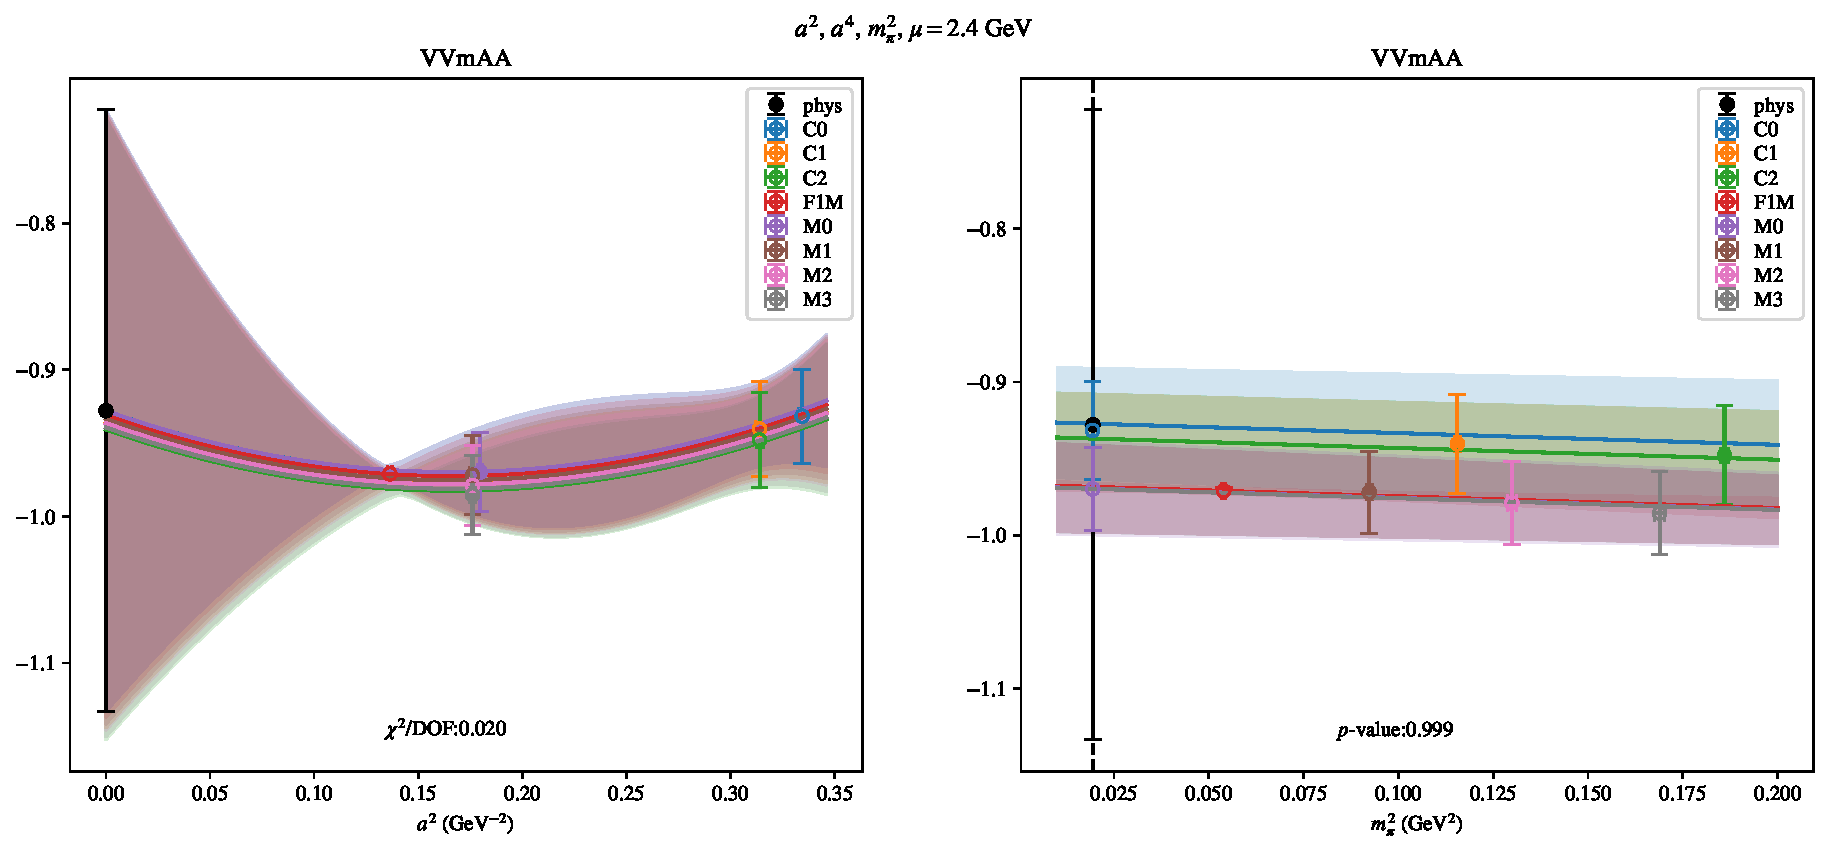
\includepdf[link, pages=-]{VVmAA/NPR/a2a4m2_24.pdf}
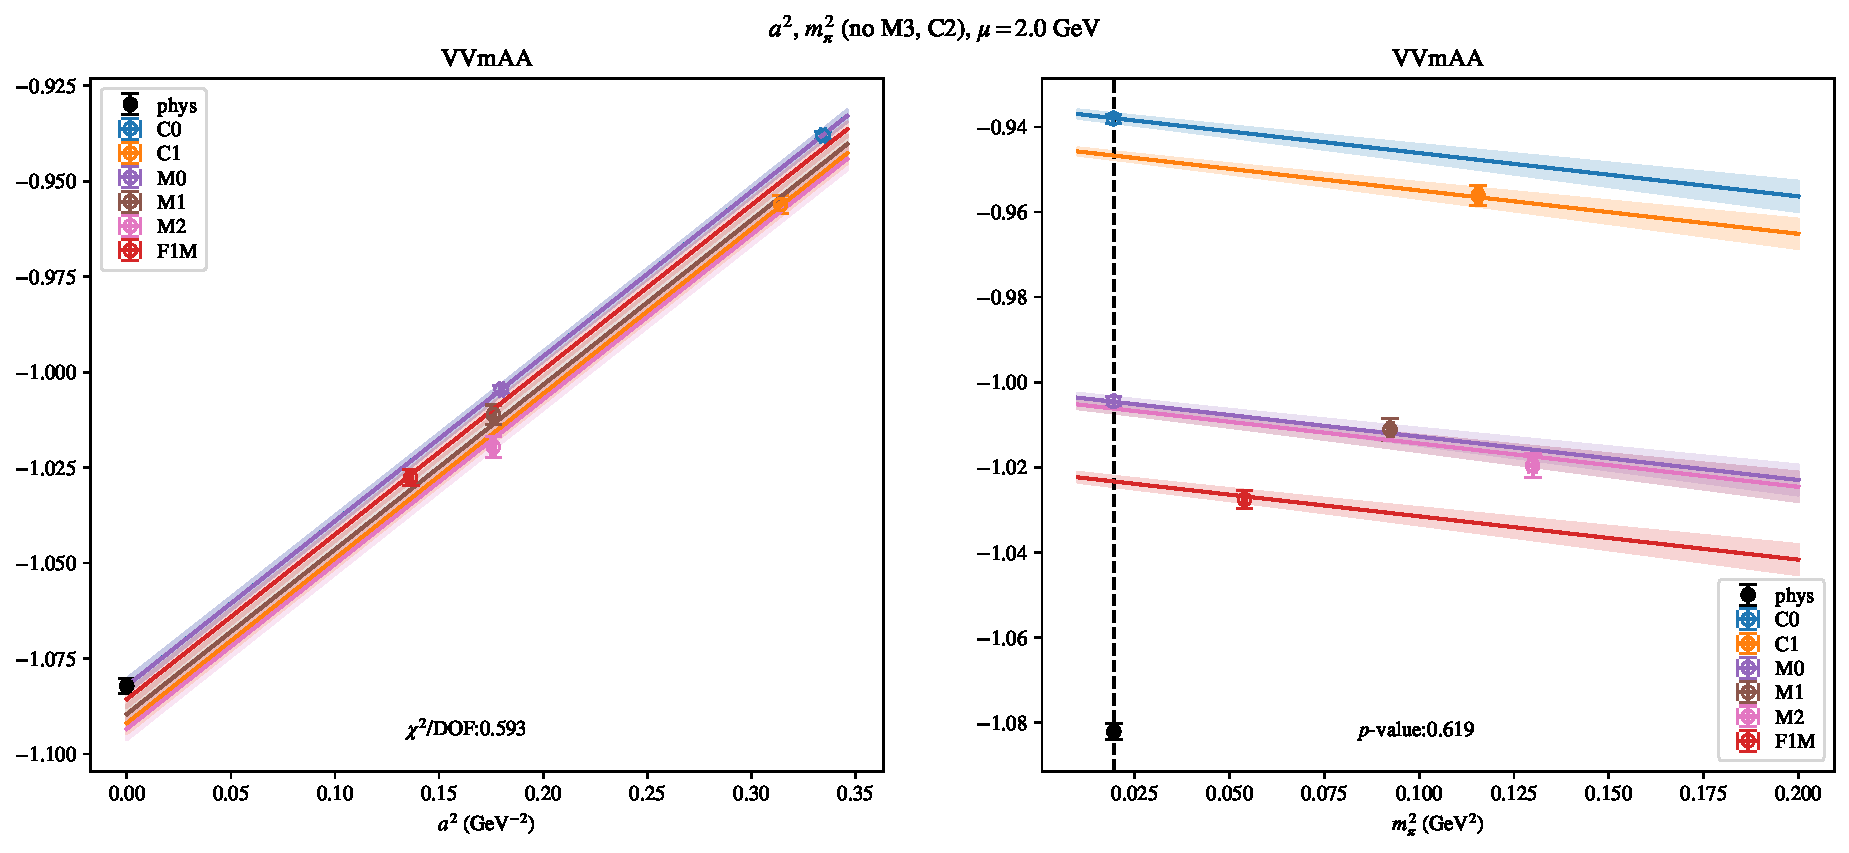
\includepdf[link, pages=-]{VVmAA/NPR/a2m2mcut_20.pdf}
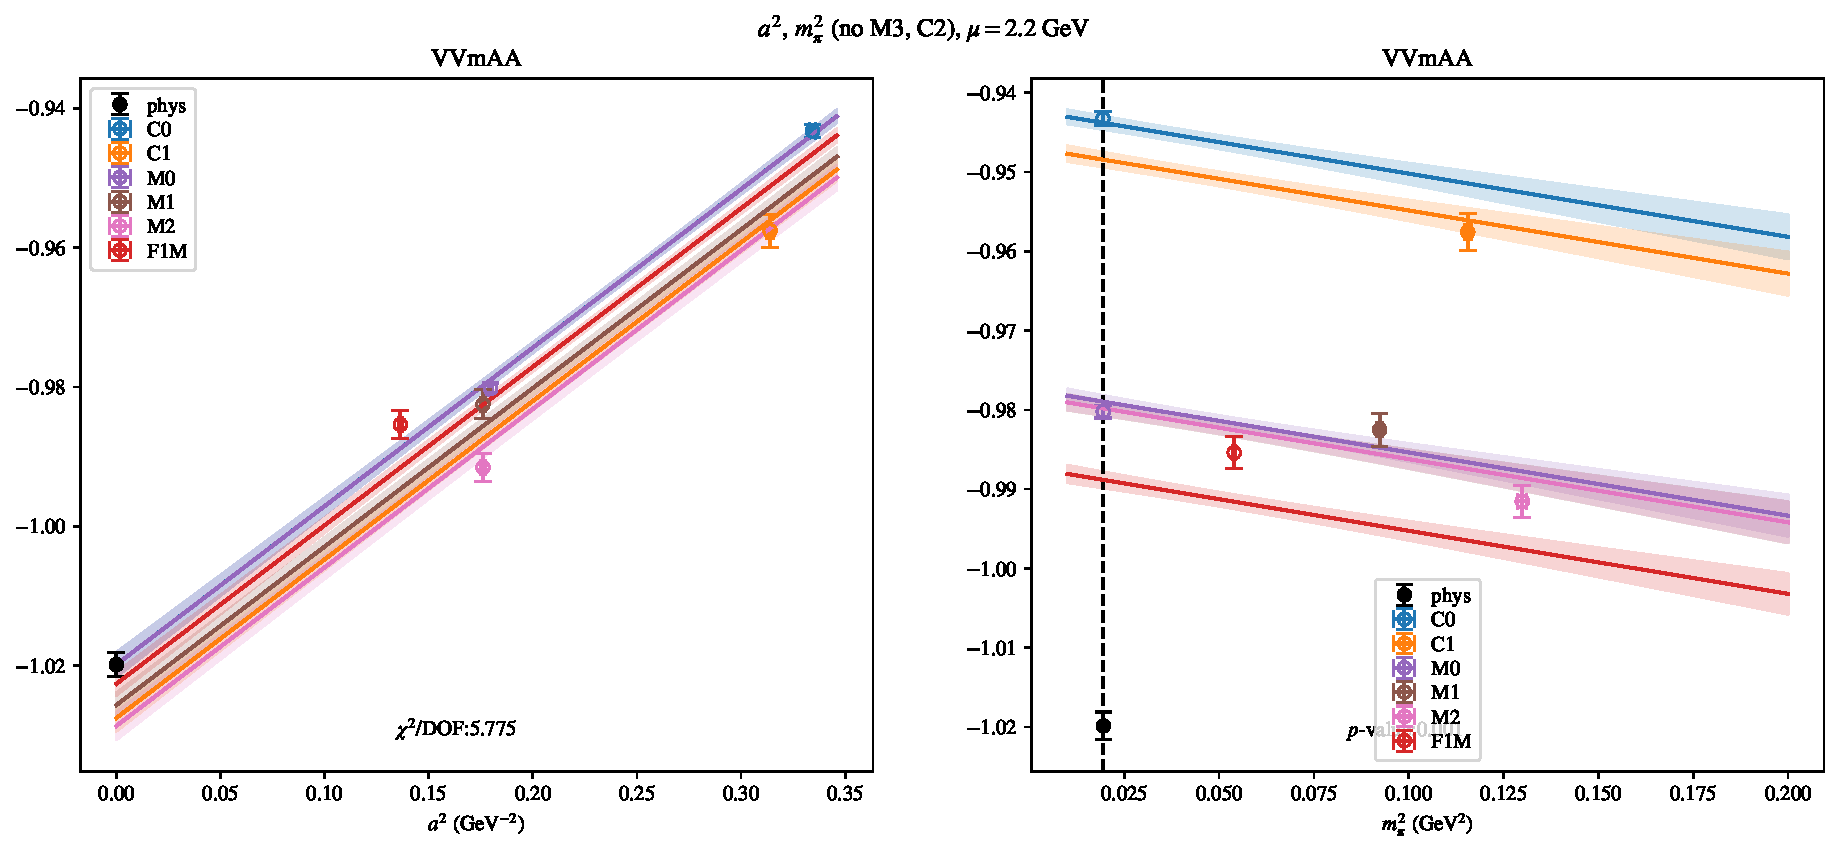
\includepdf[link, pages=-]{VVmAA/NPR/a2m2mcut_22.pdf}
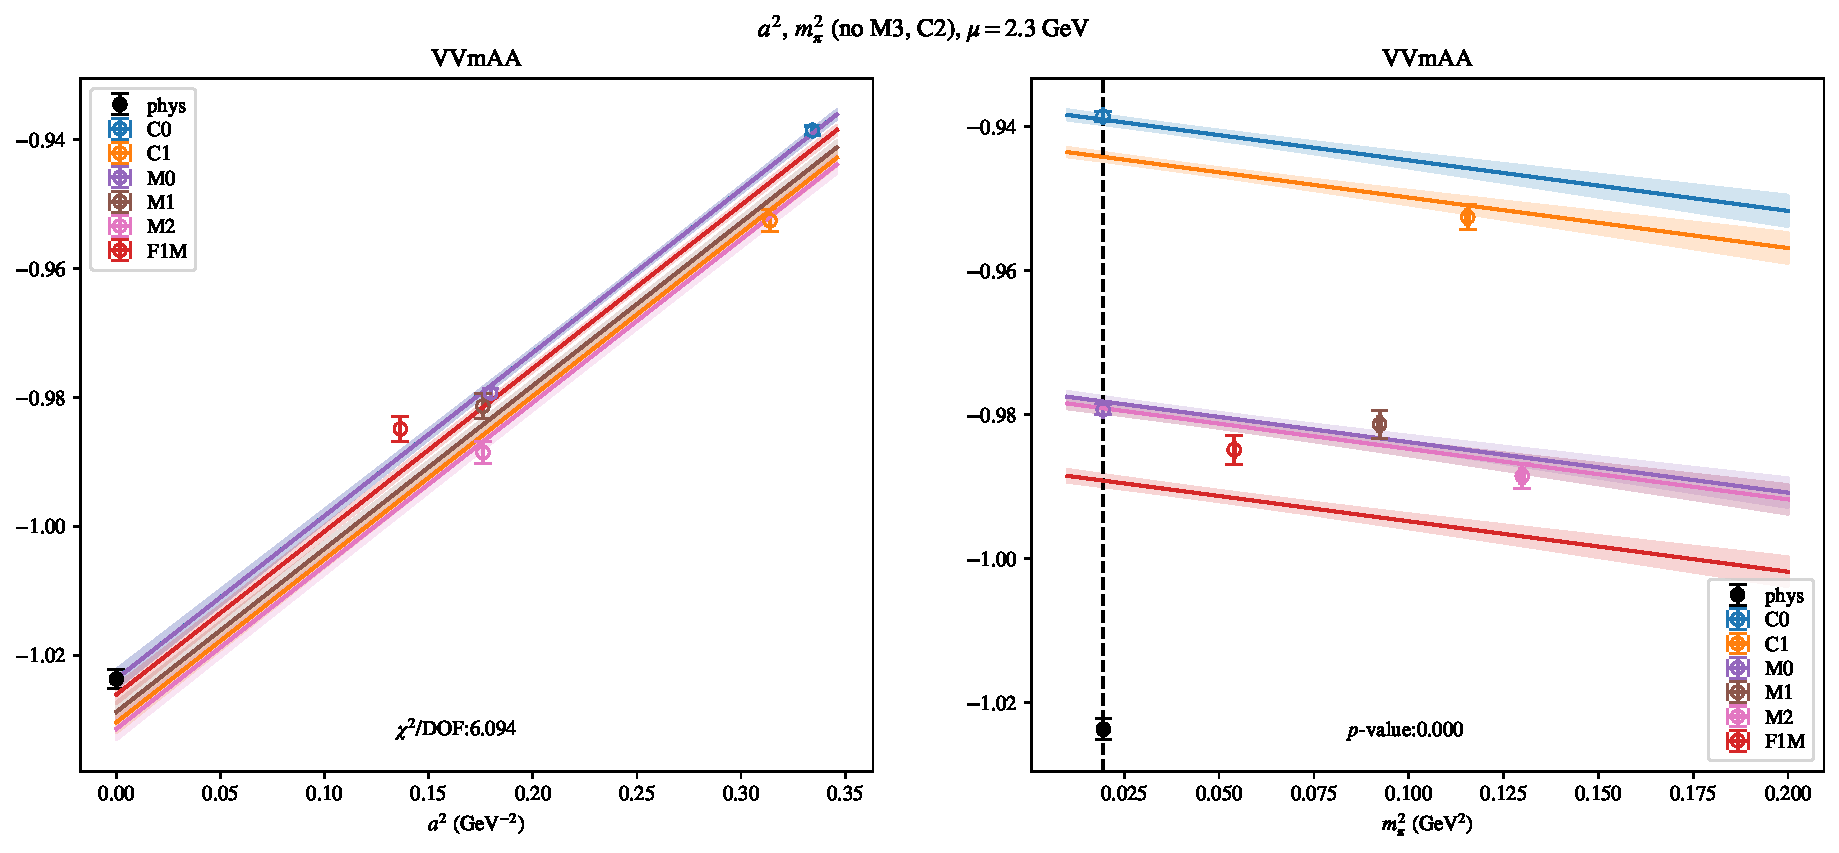
\includepdf[link, pages=-]{VVmAA/NPR/a2m2mcut_23.pdf}
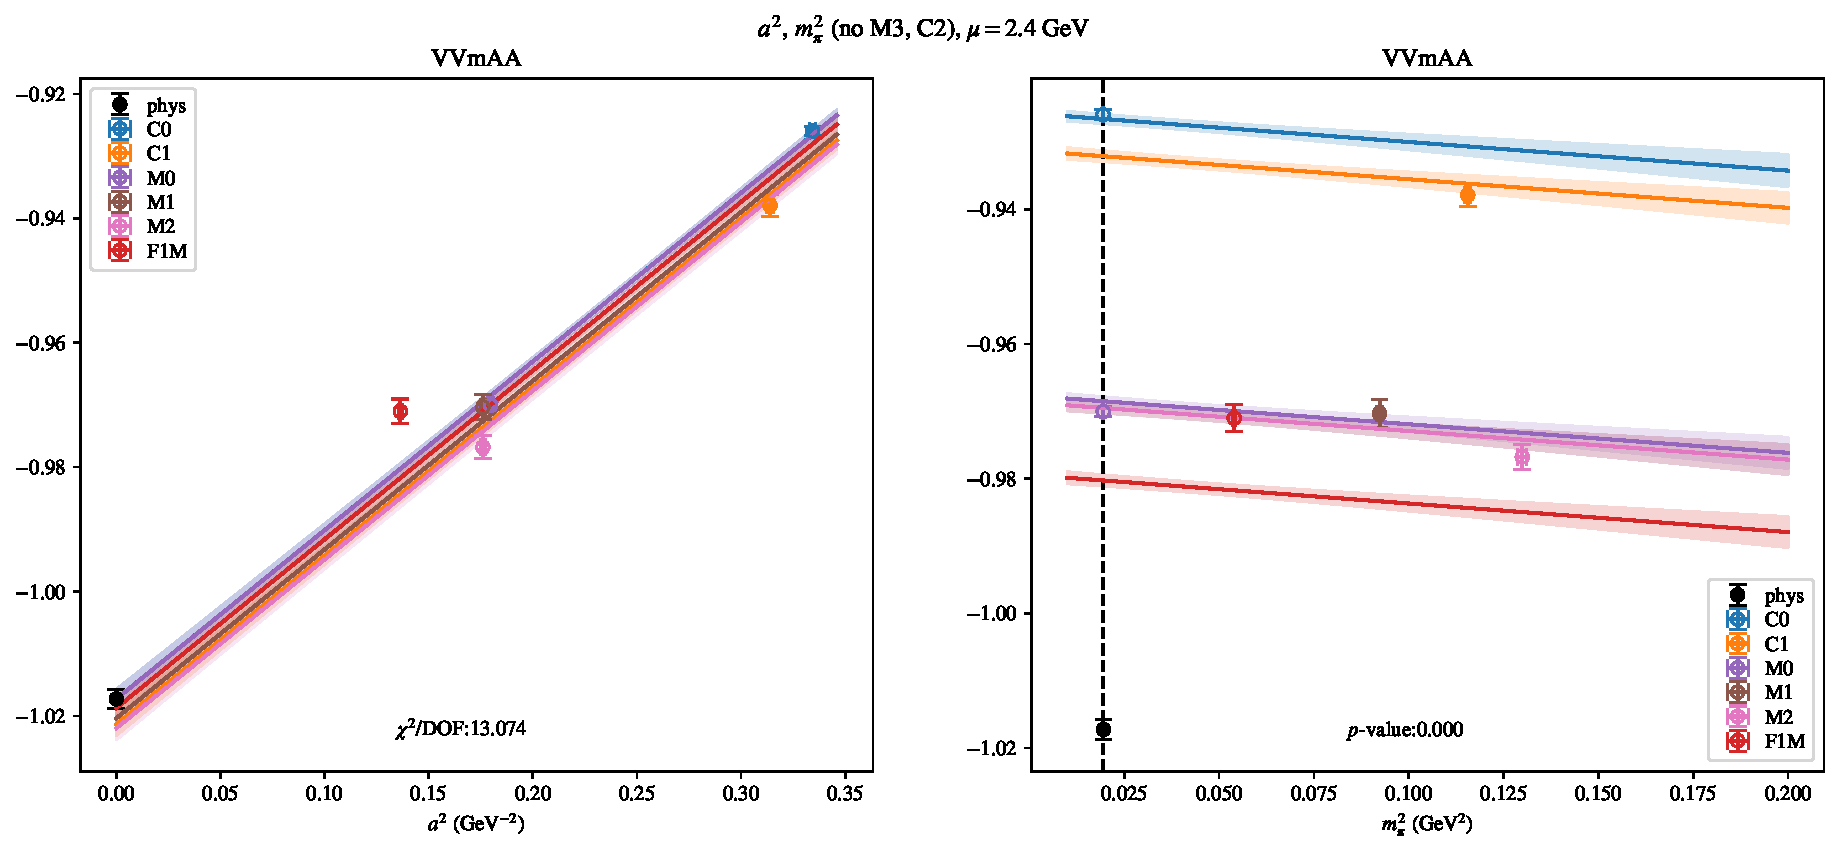
\includepdf[link, pages=-]{VVmAA/NPR/a2m2mcut_24.pdf}
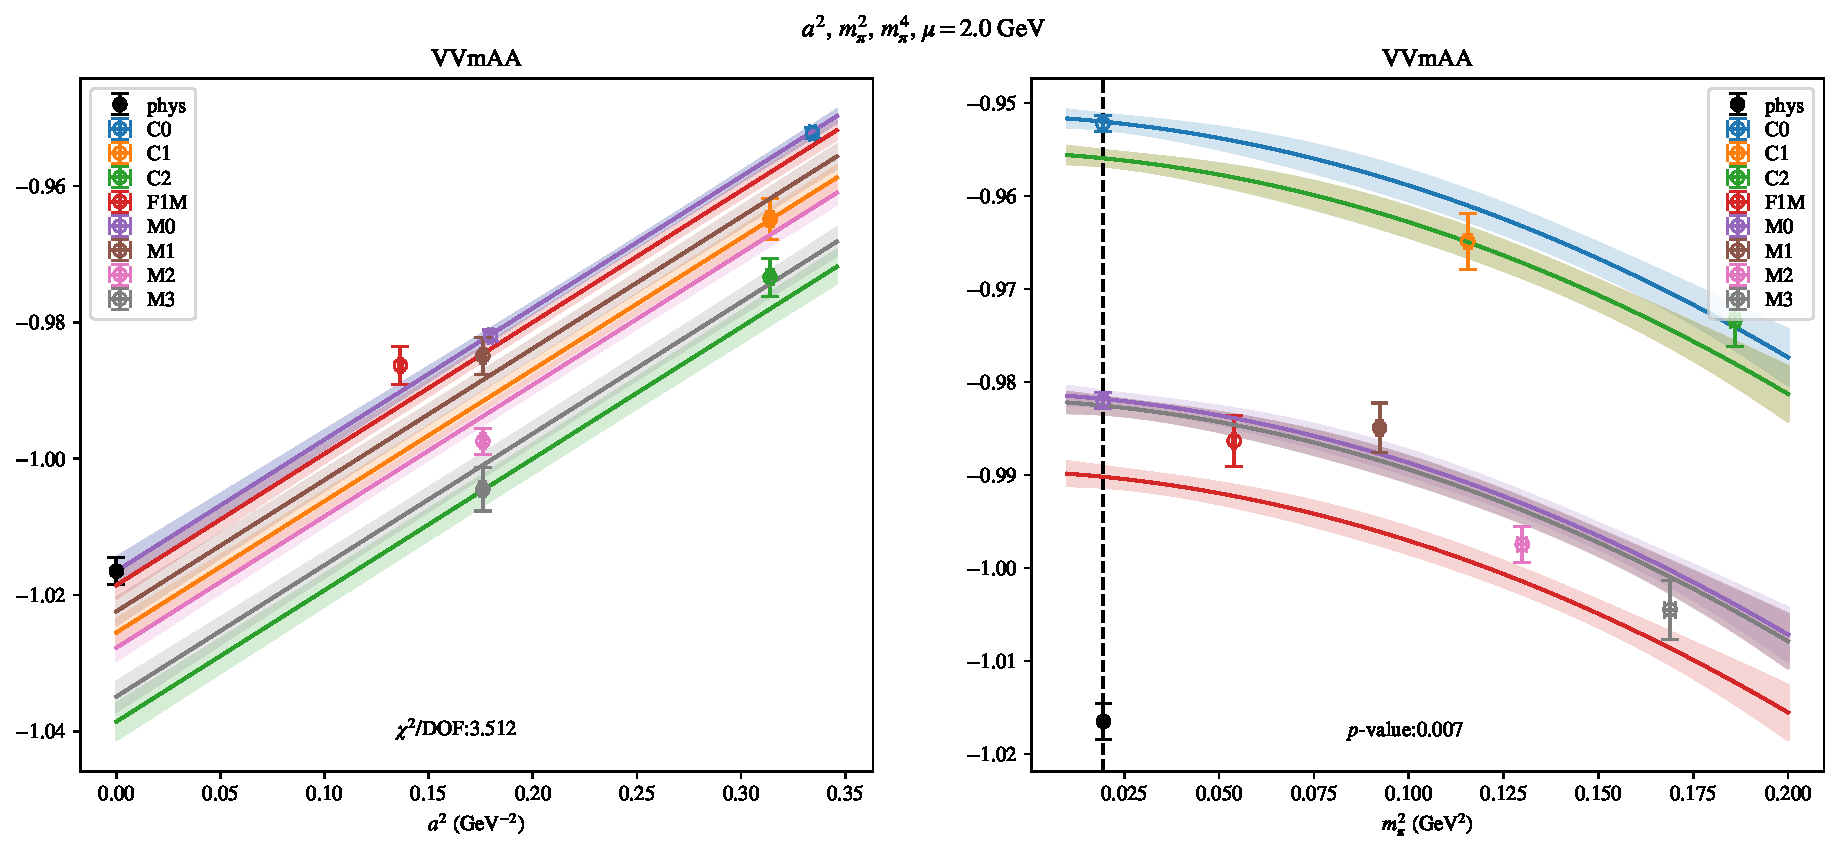
\includepdf[link, pages=-]{VVmAA/NPR/a2m2m4_20.pdf}
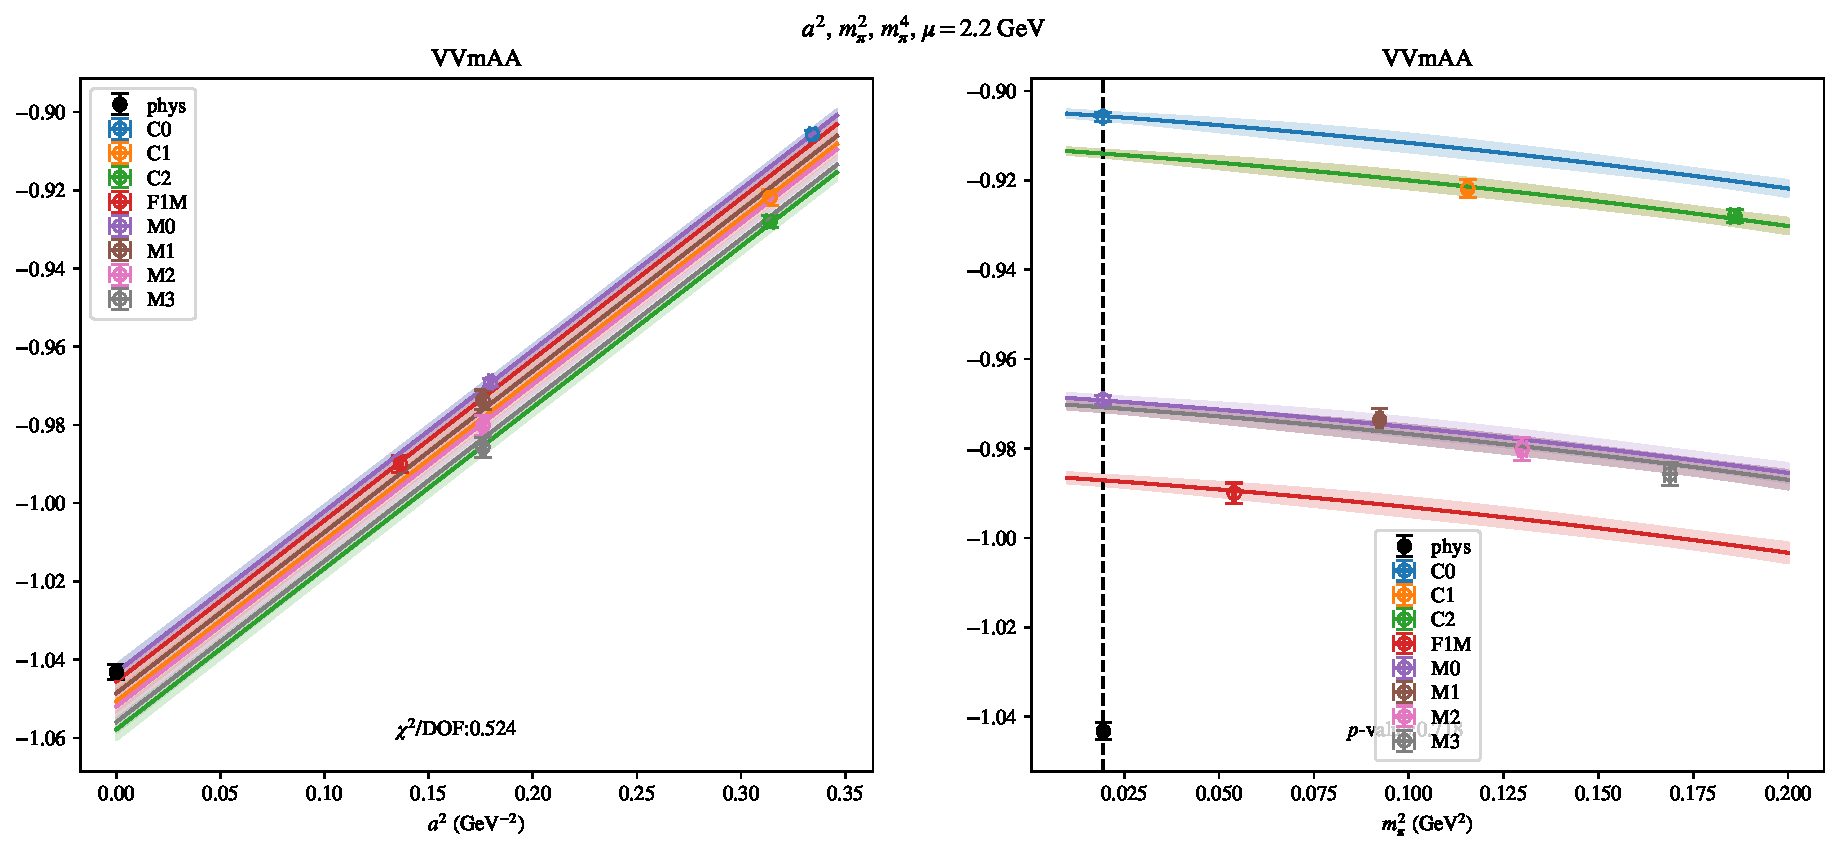
\includepdf[link, pages=-]{VVmAA/NPR/a2m2m4_22.pdf}
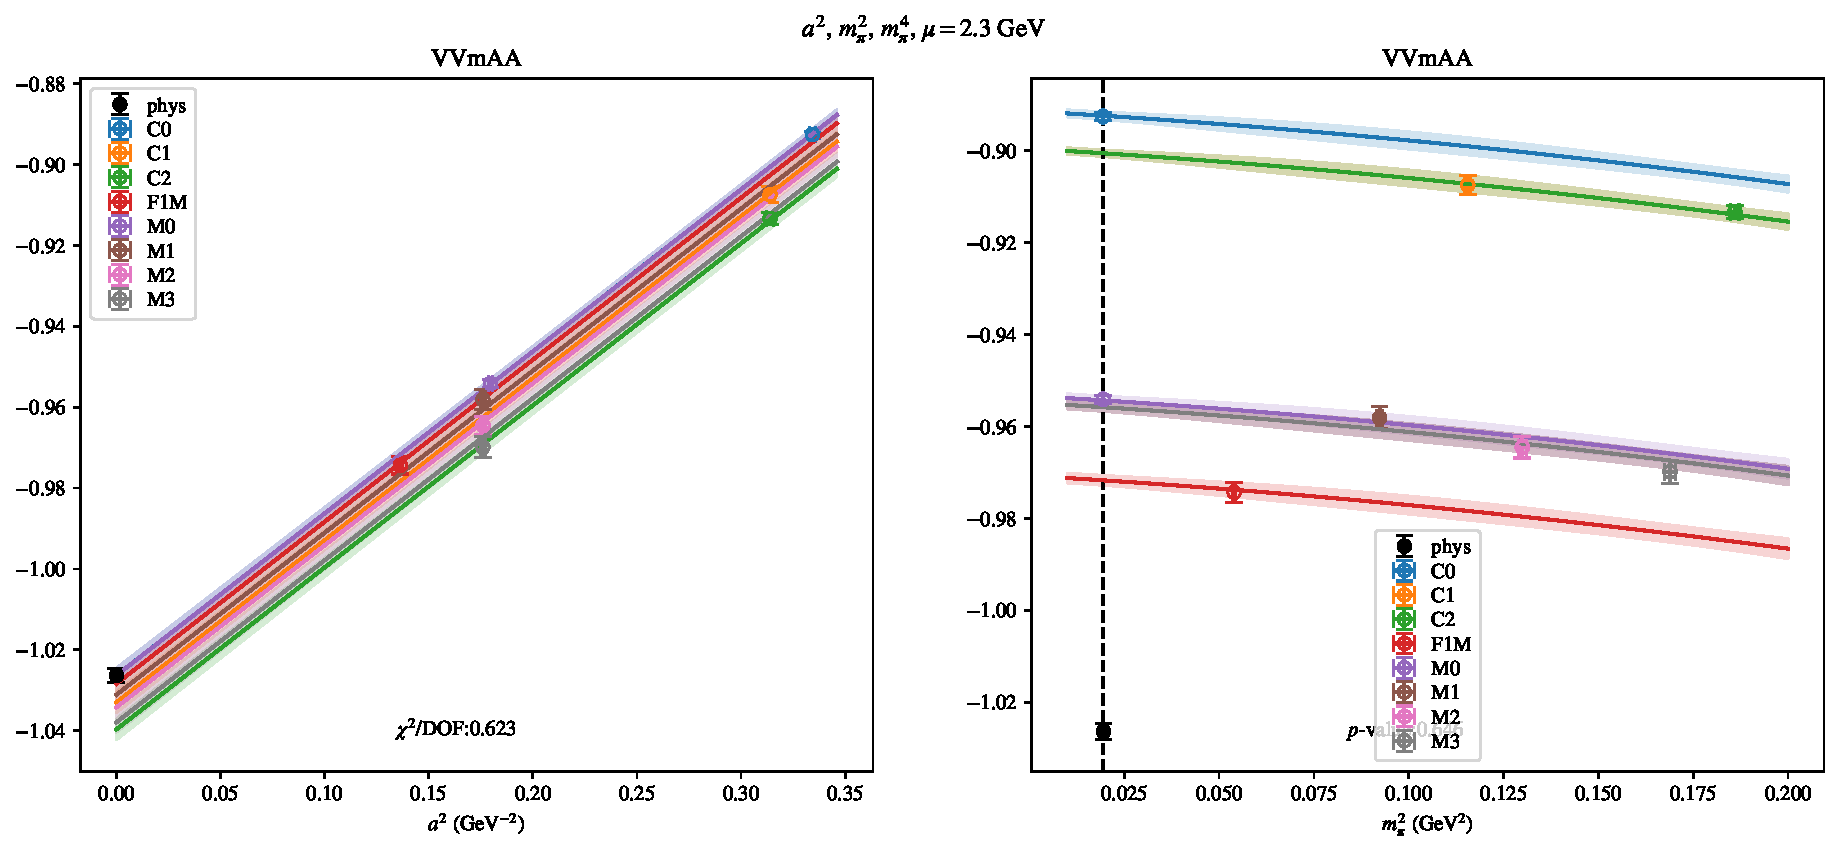
\includepdf[link, pages=-]{VVmAA/NPR/a2m2m4_23.pdf}
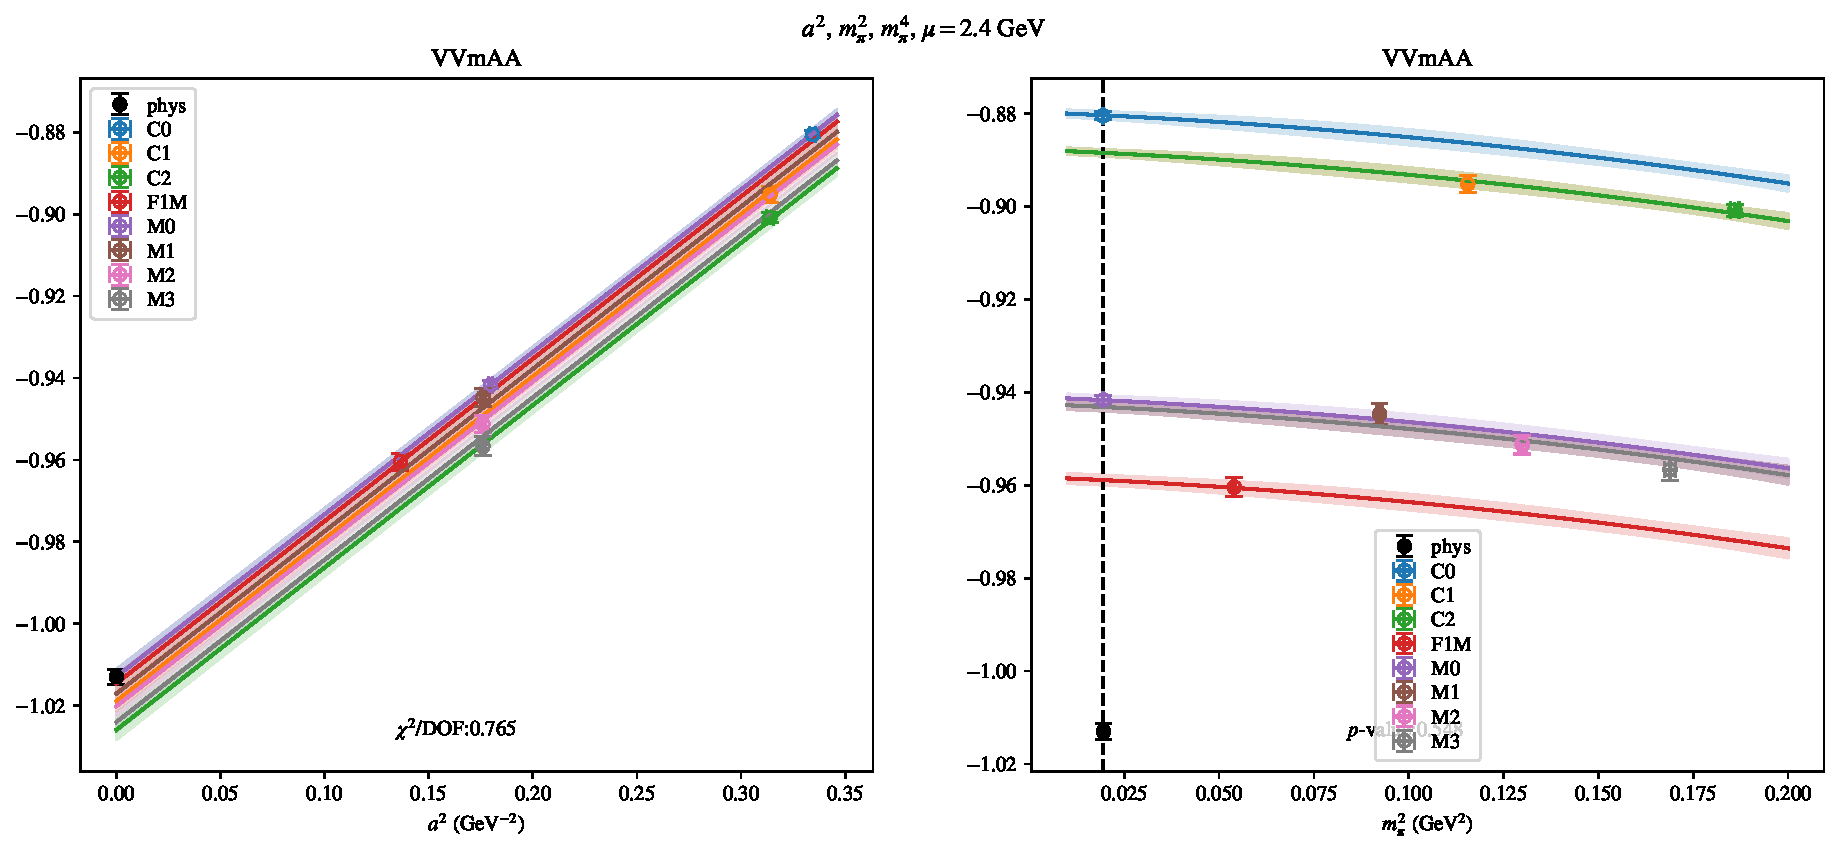
\includepdf[link, pages=-]{VVmAA/NPR/a2m2m4_24.pdf}
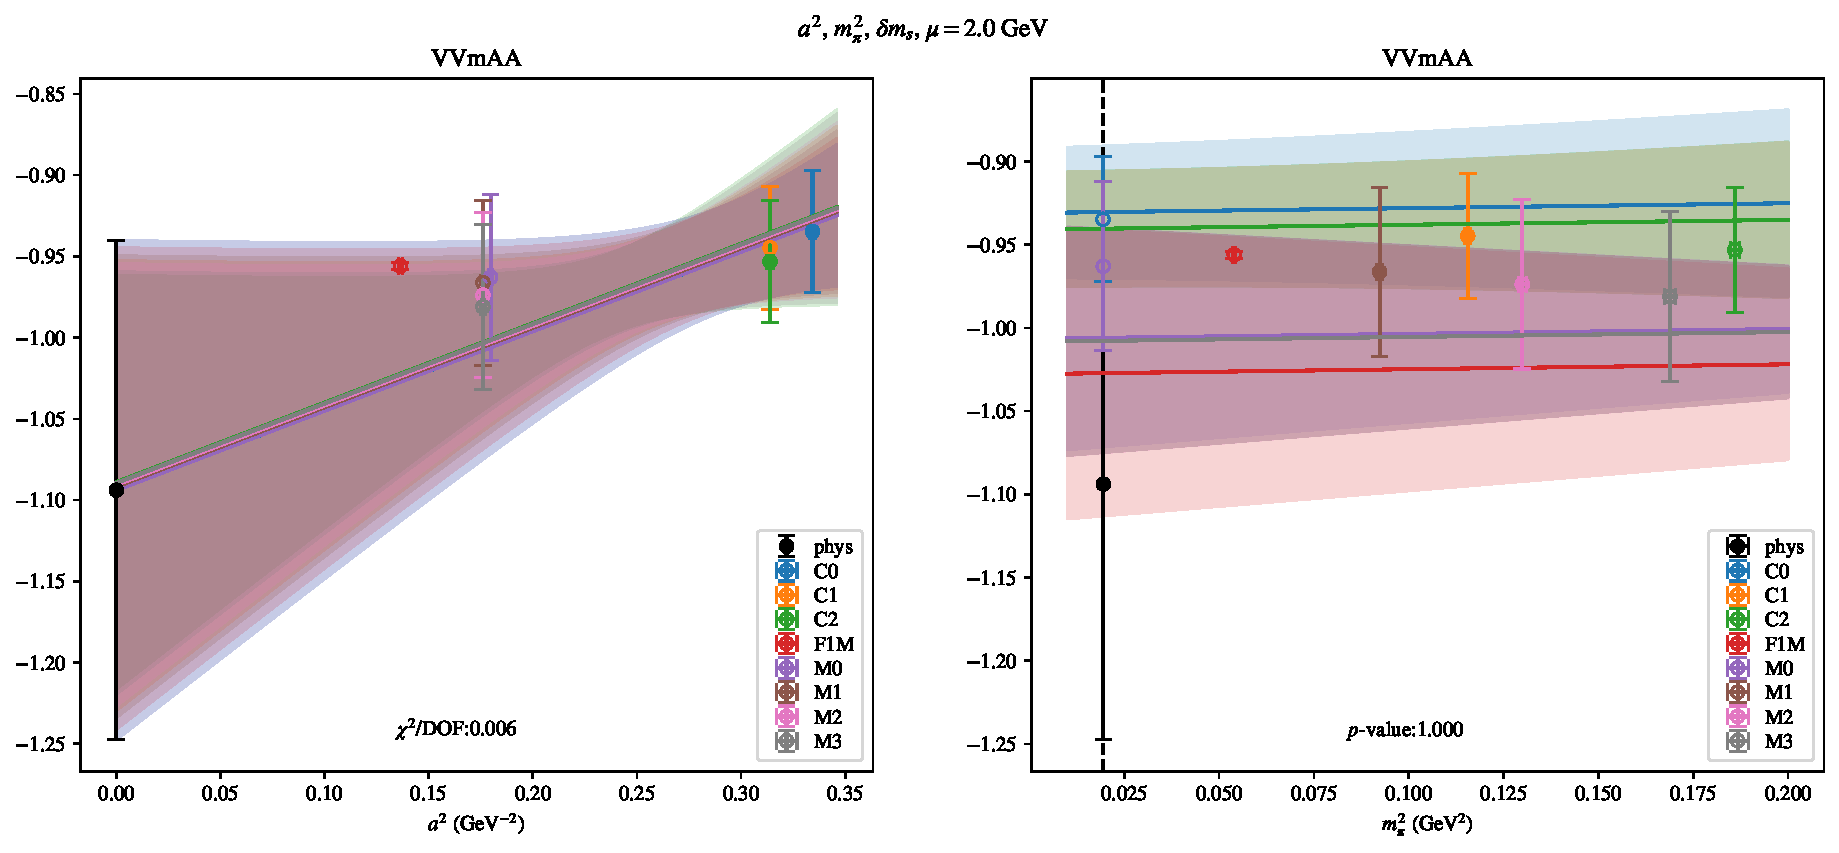
\includepdf[link, pages=-]{VVmAA/NPR/a2m2delm_20.pdf}
\includepdf[link, pages=-]{VVmAA/NPR/a2m2delm_22.pdf}
\includepdf[link, pages=-]{VVmAA/NPR/a2m2delm_23.pdf}
\includepdf[link, pages=-]{VVmAA/NPR/a2m2delm_24.pdf}
\clearpage
\section{$\mathcal{B}_3$}
\begin{table}[h!]
\begin{center}
\begin{tabular}{|c|c|c|c|c|c|c|}
\hline
$\mu$ (GeV) & $a^2$, $m_\pi^2$& $a^2$, $m_\pi^2$ (no C)& $a^2$, $a^4$, $m_\pi^2$& $a^2$, $m_\pi^2$ (no M3, C2)& $a^2$, $m_\pi^2$, $m_\pi^4$& $a^2$, $m_\pi^2$, $\delta m_s$\\
\hline
2.0& \hyperlink{SSmPP/NPR/a2m2_20.pdf.1}{\textbf{1.7632(70)}: 4.972 (0.0)} & \hyperlink{SSmPP/NPR/a2m2noC_20.pdf.1}{\textbf{1.661(27)}: 0.374 (0.688)} & \hyperlink{SSmPP/NPR/a2a4m2_20.pdf.1}{\textbf{1.543(73)}: 0.501 (0.735)} & \hyperlink{SSmPP/NPR/a2m2mcut_20.pdf.1}{\textbf{1.7574(79)}: 5.532 (0.001)} & \hyperlink{SSmPP/NPR/a2m2m4_20.pdf.1}{\textbf{1.7703(87)}: 6.078 (0.0)} & \hyperlink{SSmPP/NPR/a2m2delm_20.pdf.1}{\textbf{1.817(22)}: 0.296 (0.881)}\\
2.2& \hyperlink{SSmPP/NPR/a2m2_22.pdf.1}{\textbf{1.7859(55)}: 7.85 (0.0)} & \hyperlink{SSmPP/NPR/a2m2noC_22.pdf.1}{\textbf{1.696(20)}: 0.723 (0.485)} & \hyperlink{SSmPP/NPR/a2a4m2_22.pdf.1}{\textbf{1.613(41)}: 1.168 (0.323)} & \hyperlink{SSmPP/NPR/a2m2mcut_22.pdf.1}{\textbf{1.7820(57)}: 10.755 (0.0)} & \hyperlink{SSmPP/NPR/a2m2m4_22.pdf.1}{\textbf{1.7909(58)}: 9.127 (0.0)} & \hyperlink{SSmPP/NPR/a2m2delm_22.pdf.1}{\textbf{1.814(11)}: 0.824 (0.51)}\\
2.3& \hyperlink{SSmPP/NPR/a2m2_23.pdf.1}{\textbf{1.7874(60)}: 7.573 (0.0)} & \hyperlink{SSmPP/NPR/a2m2noC_23.pdf.1}{\textbf{1.701(18)}: 0.935 (0.392)} & \hyperlink{SSmPP/NPR/a2a4m2_23.pdf.1}{\textbf{1.622(34)}: 1.039 (0.385)} & \hyperlink{SSmPP/NPR/a2m2mcut_23.pdf.1}{\textbf{1.7875(56)}: 13.248 (0.0)} & \hyperlink{SSmPP/NPR/a2m2m4_23.pdf.1}{\textbf{1.7981(57)}: 9.584 (0.0)} & \hyperlink{SSmPP/NPR/a2m2delm_23.pdf.1}{\textbf{1.815(10)}: 1.0 (0.406)}\\
2.4& \hyperlink{SSmPP/NPR/a2m2_24.pdf.1}{\textbf{1.7934(57)}: 8.993 (0.0)} & \hyperlink{SSmPP/NPR/a2m2noC_24.pdf.1}{\textbf{1.704(16)}: 1.185 (0.306)} & \hyperlink{SSmPP/NPR/a2a4m2_24.pdf.1}{\textbf{1.626(31)}: 1.075 (0.367)} & \hyperlink{SSmPP/NPR/a2m2mcut_24.pdf.1}{\textbf{1.7899(59)}: 12.983 (0.0)} & \hyperlink{SSmPP/NPR/a2m2m4_24.pdf.1}{\textbf{1.7982(66)}: 8.613 (0.0)} & \hyperlink{SSmPP/NPR/a2m2delm_24.pdf.1}{\textbf{1.8175(97)}: 1.084 (0.363)}\\
\hline
\end{tabular}
\caption{Physical point value from chiral and continuum extrapolation at renormalisation scale $\mu$. Entries are \textbf{value(error)}: $\chi^2/\text{DOF}$ ($p$-value).}
\end{center}
\end{table}
\begin{table}[h!]
\begin{center}
\begin{tabular}{|c c|c|c|c|c|c|c|}
\hline
$\mu$ (GeV) &  & $a^2$, $m_\pi^2$& $a^2$, $m_\pi^2$ (no C)& $a^2$, $a^4$, $m_\pi^2$& $a^2$, $m_\pi^2$ (no M3, C2)& $a^2$, $m_\pi^2$, $m_\pi^4$& $a^2$, $m_\pi^2$, $\delta m_s$\\
\hline
\multirow{2}{0.5in}{2.0} & $\alpha$ & 0.133(23)& 0.57(12)& 1.62(58)& 0.148(25)& 0.123(26)& 0.042(43)\\
 & $\beta$ & 0.00036(25)& -0.0002(25)& -0.0010(34)& 0.00053(44)& -0.0017(77)& -0.0007(19)\\
\hline
\multirow{2}{0.5in}{2.2} & $\alpha$ & 0.106(12)& 0.458(84)& 1.17(29)& 0.115(13)& 0.098(13)& 0.056(20)\\
 & $\beta$ & -0.0& -0.0003(23)& -0.0009(22)& -0.0& -0.0016(73)& -0.0006(14)\\
\hline
\multirow{2}{0.5in}{2.3} & $\alpha$ & 0.112(16)& 0.448(76)& 1.12(23)& 0.118(15)& 0.096(14)& 0.064(22)\\
 & $\beta$ & -0.0& -0.0003(23)& -0.0007(15)& -0.0002(23)& -0.0026(70)& -0.0006(14)\\
\hline
\multirow{2}{0.5in}{2.4} & $\alpha$ & 0.109(15)& 0.445(67)& 1.11(21)& 0.119(15)& 0.099(16)& 0.066(21)\\
 & $\beta$ & -0.0001(14)& -0.0004(22)& -0.0007(16)& -0.0002(23)& -0.0023(69)& -0.0006(13)\\
\hline
\end{tabular}
\caption{Fit values of coefficients in $Q = Q_{phys} + \mathbf{\alpha} a^2 + \mathbf{\beta}\left(\frac{m_\pi^2}{f_\pi^2}-\frac{m_{\pi,PDG}^2}{f_\pi^2}\right) + \ldots$.}
\end{center}
\end{table}
\includepdf[link, pages=-]{SSmPP/NPR/a2m2_20.pdf}
\includepdf[link, pages=-]{SSmPP/NPR/a2m2_22.pdf}
\includepdf[link, pages=-]{SSmPP/NPR/a2m2_23.pdf}
\includepdf[link, pages=-]{SSmPP/NPR/a2m2_24.pdf}
\includepdf[link, pages=-]{SSmPP/NPR/a2m2noC_20.pdf}
\includepdf[link, pages=-]{SSmPP/NPR/a2m2noC_22.pdf}
\includepdf[link, pages=-]{SSmPP/NPR/a2m2noC_23.pdf}
\includepdf[link, pages=-]{SSmPP/NPR/a2m2noC_24.pdf}
\includepdf[link, pages=-]{SSmPP/NPR/a2a4m2_20.pdf}
\includepdf[link, pages=-]{SSmPP/NPR/a2a4m2_22.pdf}
\includepdf[link, pages=-]{SSmPP/NPR/a2a4m2_23.pdf}
\includepdf[link, pages=-]{SSmPP/NPR/a2a4m2_24.pdf}
\includepdf[link, pages=-]{SSmPP/NPR/a2m2mcut_20.pdf}
\includepdf[link, pages=-]{SSmPP/NPR/a2m2mcut_22.pdf}
\includepdf[link, pages=-]{SSmPP/NPR/a2m2mcut_23.pdf}
\includepdf[link, pages=-]{SSmPP/NPR/a2m2mcut_24.pdf}
\includepdf[link, pages=-]{SSmPP/NPR/a2m2m4_20.pdf}
\includepdf[link, pages=-]{SSmPP/NPR/a2m2m4_22.pdf}
\includepdf[link, pages=-]{SSmPP/NPR/a2m2m4_23.pdf}
\includepdf[link, pages=-]{SSmPP/NPR/a2m2m4_24.pdf}
\includepdf[link, pages=-]{SSmPP/NPR/a2m2delm_20.pdf}
\includepdf[link, pages=-]{SSmPP/NPR/a2m2delm_22.pdf}
\includepdf[link, pages=-]{SSmPP/NPR/a2m2delm_23.pdf}
\includepdf[link, pages=-]{SSmPP/NPR/a2m2delm_24.pdf}
\clearpage
\section{$\mathcal{B}_4$}
\begin{table}[h!]
\begin{center}
\begin{tabular}{|c|c|c|c|c|c|c|}
\hline
$\mu$ (GeV) & $a^2$, $m_\pi^2$& $a^2$, $m_\pi^2$ (no C)& $a^2$, $a^4$, $m_\pi^2$& $a^2$, $m_\pi^2$ (no M3, C2)& $a^2$, $m_\pi^2$, $m_\pi^4$& $a^2$, $m_\pi^2$, $\delta m_s$\\
\hline
2.0& \hyperlink{SSpPP/NPR/a2m2_20.pdf.1}{\textbf{-0.925(54)}: 0.299 (0.913)} & \hyperlink{SSpPP/NPR/a2m2noC_20.pdf.1}{\textbf{-0.91(17)}: 0.302 (0.739)} & \hyperlink{SSpPP/NPR/a2a4m2_20.pdf.1}{\textbf{-0.89(44)}: 0.178 (0.95)} & \hyperlink{SSpPP/NPR/a2m2mcut_20.pdf.1}{\textbf{-0.923(49)}: 0.383 (0.765)} & \hyperlink{SSpPP/NPR/a2m2m4_20.pdf.1}{\textbf{-0.923(63)}: 0.326 (0.861)} & \hyperlink{SSpPP/NPR/a2m2delm_20.pdf.1}{\textbf{-0.93(15)}: 0.186 (0.946)}\\
2.2& \hyperlink{SSpPP/NPR/a2m2_22.pdf.1}{\textbf{-0.907(43)}: 0.654 (0.659)} & \hyperlink{SSpPP/NPR/a2m2noC_22.pdf.1}{\textbf{-0.90(13)}: 0.587 (0.556)} & \hyperlink{SSpPP/NPR/a2a4m2_22.pdf.1}{\textbf{-0.90(27)}: 0.767 (0.546)} & \hyperlink{SSpPP/NPR/a2m2mcut_22.pdf.1}{\textbf{-0.907(38)}: 0.789 (0.5)} & \hyperlink{SSpPP/NPR/a2m2m4_22.pdf.1}{\textbf{-0.904(49)}: 0.563 (0.69)} & \hyperlink{SSpPP/NPR/a2m2delm_22.pdf.1}{\textbf{-0.906(74)}: 0.738 (0.566)}\\
2.3& \hyperlink{SSpPP/NPR/a2m2_23.pdf.1}{\textbf{-0.898(47)}: 0.716 (0.611)} & \hyperlink{SSpPP/NPR/a2m2noC_23.pdf.1}{\textbf{-0.90(12)}: 0.751 (0.472)} & \hyperlink{SSpPP/NPR/a2a4m2_23.pdf.1}{\textbf{-0.90(25)}: 0.749 (0.559)} & \hyperlink{SSpPP/NPR/a2m2mcut_23.pdf.1}{\textbf{-0.898(42)}: 0.823 (0.481)} & \hyperlink{SSpPP/NPR/a2m2m4_23.pdf.1}{\textbf{-0.895(55)}: 0.615 (0.652)} & \hyperlink{SSpPP/NPR/a2m2delm_23.pdf.1}{\textbf{-0.896(79)}: 0.734 (0.569)}\\
2.4& \hyperlink{SSpPP/NPR/a2m2_24.pdf.1}{\textbf{-0.890(49)}: 0.733 (0.599)} & \hyperlink{SSpPP/NPR/a2m2noC_24.pdf.1}{\textbf{-0.89(11)}: 0.923 (0.397)} & \hyperlink{SSpPP/NPR/a2a4m2_24.pdf.1}{\textbf{-0.90(26)}: 0.82 (0.512)} & \hyperlink{SSpPP/NPR/a2m2mcut_24.pdf.1}{\textbf{-0.890(43)}: 0.997 (0.393)} & \hyperlink{SSpPP/NPR/a2m2m4_24.pdf.1}{\textbf{-0.887(49)}: 0.744 (0.562)} & \hyperlink{SSpPP/NPR/a2m2delm_24.pdf.1}{\textbf{-0.888(71)}: 0.83 (0.506)}\\
\hline
\end{tabular}
\caption{Physical point value from chiral and continuum extrapolation at renormalisation scale $\mu$. Entries are \textbf{value(error)}: $\chi^2/\text{DOF}$ ($p$-value).}
\end{center}
\end{table}
\begin{table}[h!]
\begin{center}
\begin{tabular}{|c c|c|c|c|c|c|c|}
\hline
$\mu$ (GeV) &  & $a^2$, $m_\pi^2$& $a^2$, $m_\pi^2$ (no C)& $a^2$, $a^4$, $m_\pi^2$& $a^2$, $m_\pi^2$ (no M3, C2)& $a^2$, $m_\pi^2$, $m_\pi^4$& $a^2$, $m_\pi^2$, $\delta m_s$\\
\hline
\multirow{2}{0.5in}{2.0} & $\alpha$ & 0.394(33)& 0.50(14)& 0.74(57)& 0.398(29)& 0.401(37)& 0.373(64)\\
 & $\beta$ & 0.00706(32)& 0.00674(31)& 0.00696(20)& 0.00751(49)& 0.00836(84)& 0.00676(36)\\
\hline
\multirow{2}{0.5in}{2.2} & $\alpha$ & 0.430(23)& 0.41(10)& 0.41(32)& 0.428(21)& 0.438(26)& 0.432(33)\\
 & $\beta$ & 0.00694(17)& 0.00662(25)& 0.00698(17)& 0.00724(29)& 0.00846(80)& 0.00702(23)\\
\hline
\multirow{2}{0.5in}{2.3} & $\alpha$ & 0.457(27)& 0.419(92)& 0.37(29)& 0.454(25)& 0.466(32)& 0.464(39)\\
 & $\beta$ & 0.00692(18)& 0.00664(25)& 0.00696(19)& 0.00723(29)& 0.00845(85)& 0.00705(25)\\
\hline
\multirow{2}{0.5in}{2.4} & $\alpha$ & 0.476(29)& 0.430(86)& 0.36(30)& 0.473(26)& 0.486(29)& 0.484(36)\\
 & $\beta$ & 0.00694(19)& 0.00667(24)& 0.00694(20)& 0.00720(29)& 0.00859(81)& 0.00710(22)\\
\hline
\end{tabular}
\caption{Fit values of coefficients in $Q = Q_{phys} + \mathbf{\alpha} a^2 + \mathbf{\beta}\left(\frac{m_\pi^2}{f_\pi^2}-\frac{m_{\pi,PDG}^2}{f_\pi^2}\right) + \ldots$.}
\end{center}
\end{table}
\includepdf[link, pages=-]{SSpPP/NPR/a2m2_20.pdf}
\includepdf[link, pages=-]{SSpPP/NPR/a2m2_22.pdf}
\includepdf[link, pages=-]{SSpPP/NPR/a2m2_23.pdf}
\includepdf[link, pages=-]{SSpPP/NPR/a2m2_24.pdf}
\includepdf[link, pages=-]{SSpPP/NPR/a2m2noC_20.pdf}
\includepdf[link, pages=-]{SSpPP/NPR/a2m2noC_22.pdf}
\includepdf[link, pages=-]{SSpPP/NPR/a2m2noC_23.pdf}
\includepdf[link, pages=-]{SSpPP/NPR/a2m2noC_24.pdf}
\includepdf[link, pages=-]{SSpPP/NPR/a2a4m2_20.pdf}
\includepdf[link, pages=-]{SSpPP/NPR/a2a4m2_22.pdf}
\includepdf[link, pages=-]{SSpPP/NPR/a2a4m2_23.pdf}
\includepdf[link, pages=-]{SSpPP/NPR/a2a4m2_24.pdf}
\includepdf[link, pages=-]{SSpPP/NPR/a2m2mcut_20.pdf}
\includepdf[link, pages=-]{SSpPP/NPR/a2m2mcut_22.pdf}
\includepdf[link, pages=-]{SSpPP/NPR/a2m2mcut_23.pdf}
\includepdf[link, pages=-]{SSpPP/NPR/a2m2mcut_24.pdf}
\includepdf[link, pages=-]{SSpPP/NPR/a2m2m4_20.pdf}
\includepdf[link, pages=-]{SSpPP/NPR/a2m2m4_22.pdf}
\includepdf[link, pages=-]{SSpPP/NPR/a2m2m4_23.pdf}
\includepdf[link, pages=-]{SSpPP/NPR/a2m2m4_24.pdf}
\includepdf[link, pages=-]{SSpPP/NPR/a2m2delm_20.pdf}
\includepdf[link, pages=-]{SSpPP/NPR/a2m2delm_22.pdf}
\includepdf[link, pages=-]{SSpPP/NPR/a2m2delm_23.pdf}
\includepdf[link, pages=-]{SSpPP/NPR/a2m2delm_24.pdf}
\clearpage
\section{$\mathcal{B}_5$}
\begin{table}[h!]
\begin{center}
\begin{tabular}{|c|c|c|c|c|c|c|}
\hline
$\mu$ (GeV) & $a^2$, $m_\pi^2$& $a^2$, $m_\pi^2$ (no C)& $a^2$, $a^4$, $m_\pi^2$& $a^2$, $m_\pi^2$ (no M3, C2)& $a^2$, $m_\pi^2$, $m_\pi^4$& $a^2$, $m_\pi^2$, $\delta m_s$\\
\hline
2.0& \hyperlink{TT/NPR/a2m2_20.pdf.1}{\textbf{-0.36(16)}: 0.001 (1.0)} & \hyperlink{TT/NPR/a2m2noC_20.pdf.1}{\textbf{-0.363(78)}: 0.163 (0.849)} & \hyperlink{TT/NPR/a2a4m2_20.pdf.1}{\textbf{-0.3(21)}: 0.001 (1.0)} & \hyperlink{TT/NPR/a2m2mcut_20.pdf.1}{\textbf{-0.36(17)}: 0.001 (1.0)} & \hyperlink{TT/NPR/a2m2m4_20.pdf.1}{\textbf{-0.36(18)}: 0.001 (1.0)} & \hyperlink{TT/NPR/a2m2delm_20.pdf.1}{\textbf{-0.35(68)}: 0.001 (1.0)}\\
2.2& \hyperlink{TT/NPR/a2m2_22.pdf.1}{\textbf{-0.35(15)}: 0.006 (1.0)} & \hyperlink{TT/NPR/a2m2noC_22.pdf.1}{\textbf{-0.364(61)}: 0.248 (0.78)} & \hyperlink{TT/NPR/a2a4m2_22.pdf.1}{\textbf{-0.3(12)}: 0.001 (1.0)} & \hyperlink{TT/NPR/a2m2mcut_22.pdf.1}{\textbf{-0.35(15)}: 0.009 (0.999)} & \hyperlink{TT/NPR/a2m2m4_22.pdf.1}{\textbf{-0.35(14)}: 0.007 (1.0)} & \hyperlink{TT/NPR/a2m2delm_22.pdf.1}{\textbf{-0.35(49)}: 0.002 (1.0)}\\
2.3& \hyperlink{TT/NPR/a2m2_23.pdf.1}{\textbf{-0.35(12)}: 0.007 (1.0)} & \hyperlink{TT/NPR/a2m2noC_23.pdf.1}{\textbf{-0.362(56)}: 0.304 (0.738)} & \hyperlink{TT/NPR/a2a4m2_23.pdf.1}{\textbf{-0.3(11)}: 0.002 (1.0)} & \hyperlink{TT/NPR/a2m2mcut_23.pdf.1}{\textbf{-0.35(13)}: 0.009 (0.999)} & \hyperlink{TT/NPR/a2m2m4_23.pdf.1}{\textbf{-0.35(14)}: 0.008 (1.0)} & \hyperlink{TT/NPR/a2m2delm_23.pdf.1}{\textbf{-0.35(41)}: 0.002 (1.0)}\\
2.4& \hyperlink{TT/NPR/a2m2_24.pdf.1}{\textbf{-0.35(13)}: 0.007 (1.0)} & \hyperlink{TT/NPR/a2m2noC_24.pdf.1}{\textbf{-0.360(53)}: 0.344 (0.709)} & \hyperlink{TT/NPR/a2a4m2_24.pdf.1}{\textbf{-0.36(94)}: 0.002 (1.0)} & \hyperlink{TT/NPR/a2m2mcut_24.pdf.1}{\textbf{-0.35(13)}: 0.009 (0.999)} & \hyperlink{TT/NPR/a2m2m4_24.pdf.1}{\textbf{-0.35(14)}: 0.007 (1.0)} & \hyperlink{TT/NPR/a2m2delm_24.pdf.1}{\textbf{-0.35(35)}: 0.003 (1.0)}\\
\hline
\end{tabular}
\caption{Physical point value from chiral and continuum extrapolation at renormalisation scale $\mu$. Entries are \textbf{value(error)}: $\chi^2/\text{DOF}$ ($p$-value).}
\end{center}
\end{table}
\begin{table}[h!]
\begin{center}
\begin{tabular}{|c c|c|c|c|c|c|c|}
\hline
$\mu$ (GeV) &  & $a^2$, $m_\pi^2$& $a^2$, $m_\pi^2$ (no C)& $a^2$, $a^4$, $m_\pi^2$& $a^2$, $m_\pi^2$ (no M3, C2)& $a^2$, $m_\pi^2$, $m_\pi^4$& $a^2$, $m_\pi^2$, $\delta m_s$\\
\hline
\multirow{2}{0.5in}{2.0} & $\alpha$ & 0.001& -0.048& -0.127& 0.001& 0.003& 0.01\\
 & $\beta$ & 0.0062(47)& 0.00658(30)& 0.0063(58)& 0.0061(61)& 0.0067(38)& 0.0064(48)\\
\hline
\multirow{2}{0.5in}{2.2} & $\alpha$ & -0.058& -0.1(10)& -0.401& -0.06& -0.052& -0.028\\
 & $\beta$ & 0.0058(41)& 0.00634(25)& 0.006& 0.0057(46)& 0.0066(31)& 0.0063(29)\\
\hline
\multirow{2}{0.5in}{2.3} & $\alpha$ & -0.069& -0.17(99)& -0.383& -0.071& -0.065& -0.043\\
 & $\beta$ & 0.0058(35)& 0.00632(24)& 0.0061(16)& 0.0057(44)& 0.0068(31)& 0.0063(23)\\
\hline
\multirow{2}{0.5in}{2.4} & $\alpha$ & -0.093& -0.18(94)& -0.354& -0.093& -0.086& -0.068\\
 & $\beta$ & 0.0058(34)& 0.00630(24)& 0.0060(15)& 0.0057(42)& 0.0068(32)& 0.0062(18)\\
\hline
\end{tabular}
\caption{Fit values of coefficients in $Q = Q_{phys} + \mathbf{\alpha} a^2 + \mathbf{\beta}\left(\frac{m_\pi^2}{f_\pi^2}-\frac{m_{\pi,PDG}^2}{f_\pi^2}\right) + \ldots$.}
\end{center}
\end{table}
\includepdf[link, pages=-]{TT/NPR/a2m2_20.pdf}
\includepdf[link, pages=-]{TT/NPR/a2m2_22.pdf}
\includepdf[link, pages=-]{TT/NPR/a2m2_23.pdf}
\includepdf[link, pages=-]{TT/NPR/a2m2_24.pdf}
\includepdf[link, pages=-]{TT/NPR/a2m2noC_20.pdf}
\includepdf[link, pages=-]{TT/NPR/a2m2noC_22.pdf}
\includepdf[link, pages=-]{TT/NPR/a2m2noC_23.pdf}
\includepdf[link, pages=-]{TT/NPR/a2m2noC_24.pdf}
\includepdf[link, pages=-]{TT/NPR/a2a4m2_20.pdf}
\includepdf[link, pages=-]{TT/NPR/a2a4m2_22.pdf}
\includepdf[link, pages=-]{TT/NPR/a2a4m2_23.pdf}
\includepdf[link, pages=-]{TT/NPR/a2a4m2_24.pdf}
\includepdf[link, pages=-]{TT/NPR/a2m2mcut_20.pdf}
\includepdf[link, pages=-]{TT/NPR/a2m2mcut_22.pdf}
\includepdf[link, pages=-]{TT/NPR/a2m2mcut_23.pdf}
\includepdf[link, pages=-]{TT/NPR/a2m2mcut_24.pdf}
\includepdf[link, pages=-]{TT/NPR/a2m2m4_20.pdf}
\includepdf[link, pages=-]{TT/NPR/a2m2m4_22.pdf}
\includepdf[link, pages=-]{TT/NPR/a2m2m4_23.pdf}
\includepdf[link, pages=-]{TT/NPR/a2m2m4_24.pdf}
\includepdf[link, pages=-]{TT/NPR/a2m2delm_20.pdf}
\includepdf[link, pages=-]{TT/NPR/a2m2delm_22.pdf}
\includepdf[link, pages=-]{TT/NPR/a2m2delm_23.pdf}
\includepdf[link, pages=-]{TT/NPR/a2m2delm_24.pdf}
\clearpage
\end{document}